%% LyX 2.3.6.1 created this file.  For more info, see http://www.lyx.org/.
%% Do not edit unless you really know what you are doing.
\documentclass[11pt,oneside,american,czech]{book}
\usepackage[T1]{fontenc}
\usepackage[utf8]{inputenc}
\usepackage[a4paper]{geometry}
\geometry{verbose,tmargin=4cm,bmargin=3cm,lmargin=3cm,rmargin=2cm,headheight=0.8cm,headsep=1cm,footskip=0.5cm}
\pagestyle{headings}
\setcounter{secnumdepth}{3}
\usepackage{url}
\usepackage{amsmath}
\usepackage{amsthm}
\usepackage{amssymb}
\usepackage{graphicx}
\usepackage{setspace}
\usepackage{caption}
\usepackage{subcaption}
\usepackage{listings}
\usepackage[dvipsnames,table,xcdraw]{xcolor}
\usepackage[T1]{fontenc}
\usepackage{lmodern}
\usepackage{pdfpages}
\usepackage{longtable}
\usepackage{multirow}
\usepackage{hyperref}
\hypersetup{
    colorlinks=true,
    linkcolor=violet,
    filecolor=magenta,      
    urlcolor=cyan,
    pdftitle={Moderní metody robustního strojového učení},
    pdfpagemode=FullScreen,
    }

\definecolor{mygreen}{rgb}{0,0.6,0}
\definecolor{mygray}{rgb}{0.5,0.5,0.5}
\definecolor{mymauve}{rgb}{0.58,0,0.82}
\definecolor{mystring}{rgb}{0.9,0.1,0.2}

\lstset{ 
  backgroundcolor=\color{white},   % choose the background color; you must add \usepackage{color} or \usepackage{xcolor}; should come as last argument
  basicstyle=\scriptsize\fontfamily{cmtt}\selectfont,        % the size of the fonts that are used for the code
  breakatwhitespace=false,         % sets if automatic breaks should only happen at whitespace
  breaklines=true,                 % sets automatic line breaking
  captionpos=t,                    % sets the caption-position to bottom
  commentstyle=\color{mygreen},    % comment style
  stringstyle=\color{mystring},
  deletekeywords={...},            % if you want to delete keywords from the given language
  escapeinside={\%*}{*)},          % if you want to add LaTeX within your code
  extendedchars=true,              % lets you use non-ASCII characters; for 8-bits encodings only, does not work with UTF-8
  firstnumber=1,                   % start line enumeration with line 1000
  frame=single,	                   % adds a frame around the code
  keepspaces=true,                 % keeps spaces in text, useful for keeping indentation of code (possibly needs columns=flexible)
  keywordstyle=\color{blue},       % keyword style
  language=Python,                 % the language of the code
  morekeywords={*,...},            % if you want to add more keywords to the set
  numbers=left,                    % where to put the line-numbers; possible values are (none, left, right)
  numbersep=5pt,                   % how far the line-numbers are from the code
  numberstyle=\tiny\color{mygray}, % the style that is used for the line-numbers
  rulecolor=\color{black},         % if not set, the frame-color may be changed on line-breaks within not-black text (e.g. comments (green here))
  showspaces=false,                % show spaces everywhere adding particular underscores; it overrides 'showstringspaces'
  showstringspaces=false,          % underline spaces within strings only
  showtabs=false,                  % show tabs within strings adding particular underscores
  stepnumber=2,                    % the step between two line-numbers. If it's 1, each line will be numbered
  stringstyle=\color{mymauve},     % string literal style
  tabsize=2,	                   % sets default tabsize to 2 spaces
  title=\lstname                   % show the filename of files included with \lstinputlisting; also try caption instead of title
}

\makeatletter
%%%%%%%%%%%%%%%%%%%%%%%%%%%%%% Textclass specific LaTeX commands.
\newenvironment{lyxlist}[1]
	{\begin{list}{}
		{\settowidth{\labelwidth}{#1}
		 \setlength{\leftmargin}{\labelwidth}
		 \addtolength{\leftmargin}{\labelsep}
		 \renewcommand{\makelabel}[1]{##1\hfil}}}
	{\end{list}}

%%%%%%%%%%%%%%%%%%%%%%%%%%%%%% User specified LaTeX commands.
%% Font setup: please leave the LyX font settings all set to 'default'
%% if you want to use any of these packages:

%% Use Times New Roman font for text and Belleek font for math
%% Please make sure that the 'esint' package is turned off in the
%% 'Math options' page.
\usepackage[varg]{txfonts}

%% Use Utopia text with Fourier-GUTenberg math
%\usepackage{fourier}

%% Bitstream Charter text with Math Design math
%\usepackage[charter]{mathdesign}

%%---------------------------------------------------------------------

%% Make the multiline figure/table captions indent so that the second
%% line "hangs" right below the first one.
%\usepackage[format=hang]{caption}

%% Indent even the first paragraph in each section
\usepackage{indentfirst}

%%---------------------------------------------------------------------

%% Disable page numbers in the TOC. LOF, LOT (TOC automatically
%% adds \thispagestyle{chapter} if not overriden
%\addtocontents{toc}{\protect\thispagestyle{empty}}
%\addtocontents{lof}{\protect\thispagestyle{empty}}
%\addtocontents{lot}{\protect\thispagestyle{empty}}

%% Shifts the top line of the TOC (not the title) 1cm upwards 
%% so that the whole TOC fits on 1 page. Additional page size
%% adjustment is performed at the point where the TOC
%% is inserted.
%\addtocontents{toc}{\protect\vspace{-1cm}}

%%---------------------------------------------------------------------

% completely avoid orphans (first lines of a new paragraph on the bottom of a page)
\clubpenalty=9500

% completely avoid widows (last lines of paragraph on a new page)
\widowpenalty=9500

% disable hyphenation of acronyms
\hyphenation{CDFA HARDI HiPPIES IKEM InterTrack MEGIDDO MIMD MPFA DICOM ASCLEPIOS MedInria}

%%---------------------------------------------------------------------

%% Print out all vectors in bold type instead of printing an arrow above them
\renewcommand{\vec}[1]{\boldsymbol{#1}}

% Replace standard \cite by the parenthetical variant \citep
%\renewcommand{\cite}{\citep}

\makeatother

\usepackage{babel}

\newtheorem{theorem}{Tvrzení}[section]
\newtheorem{definition}{Definice}[section]
\newtheorem{lemma}[definition]{Lemma}

\begin{document}
\def\documentdate{10. května 2024}

%%\def\documentdate{\today}

\pagestyle{empty}
{\centering

\noindent %
\begin{minipage}[c]{3cm}%
\noindent \begin{center}

\includegraphics[width=3cm,height=3cm,keepaspectratio]{Images/TITLE/cvut}
\par\end{center}%
\end{minipage}%
\begin{minipage}[c]{0.6\linewidth}%
\begin{center}
\textsc{\large{}České vysoké učení technické v Praze}{\large{}}\\
{\large{}Fakulta jaderná a fyzikálně inženýrská}
\par\end{center}%
\end{minipage}%
\begin{minipage}[c]{3cm}%
\noindent \begin{center}

\includegraphics[width=3cm,height=3cm,keepaspectratio]{Images/TITLE/fjfi}
\par\end{center}%
\end{minipage}

\vspace{3cm}

\textbf{\huge{}Moderní metody robustního strojového učení}{\huge\par}

\vspace{1cm}

\selectlanguage{american}%
\textbf{\huge{}Modern methods of robust machine learning}{\huge\par}

\selectlanguage{czech}%
\vspace{2cm}

{\large{}Diplomová práce}{\large\par}

}

\vfill{}

\begin{lyxlist}{MMMMMMMMM}
\begin{singlespace}
\item [{Autor:}] \textbf{Bc. Pavel Jakš}
\item [{Vedoucí~práce:}] \textbf{Mgr. Lukáš Adam, Ph.D.}
\item [{Konzultant:}] \textbf{Ing. Pavel Strachota, Ph.D.}
\item [{Akademický~rok:}] 2023/2024
\end{singlespace}
\end{lyxlist}
\newpage{}

\includepdf{zadani_dp2.pdf}

\includepdf[page=2]{zadani_dp.pdf}

\newpage{}

\noindent \emph{\Large{}Poděkování:}{\Large\par}

\noindent Chtěl bych zde poděkovat především svému školiteli panu doktoru Adamovi
za pečlivost, ochotu, vstřícnost a odborné i lidské zázemí při vedení
mé diplomové práce. Dále děkuji svému konzultantovi panu doktoru Strachotovi
za jeho odborné rady.

\vfill

\noindent \emph{\Large{}Čestné prohlášení:}{\Large\par}

\noindent Prohlašuji, že jsem tuto práci vypracoval samostatně a uvedl
jsem všechnu použitou literaturu.

\bigskip{}

\noindent V Praze dne 10. května 2024\hfill{}Bc. Pavel Jakš

\vspace{2cm}

\newpage{}

\begin{onehalfspace}
\noindent \emph{Název práce:}

\noindent \textbf{Moderní metody robustního strojového učení}
\end{onehalfspace}

\bigskip{}

\noindent \emph{Autor:} Bc. Pavel Jakš

\bigskip{}

\noindent \emph{Studijní program:} Matematická informatika\bigskip{}

\bigskip{}

\noindent \emph{Druh práce:} Diplomová práce

\bigskip{}

\noindent \emph{Vedoucí práce:} Mgr. Lukáš Adam, Ph.D.,
Ministerstvo životního prostředí České republiky,
Vršovická 1442/65, Vršovice, 100 10 Praha 10

\bigskip{}

\noindent \emph{Konzultant:} Ing. Pavel Strachota, Ph.D.,
Katedra matematiky,
Fakulta jaderná a fyzikálně inženýrská,
České vysoké učení technické v Praze,
Trojanova 13, 120 00 Praha 2.

\bigskip{}

\noindent \emph{Abstrakt:}
V oblasti strojového učení se vyskytl problém existence tak zvaných adversariálních vzorků.
Jedná se o jev, kdy i malá změna vstupu nějakého modelu strojového učení
způsobí velikou změnu výstupu, což je ve většině případech nežádoucí.
V této práci se potom věnujeme problematice metrik vizuální podobnosti,
a to právě v kontextu existence a tvorby adversariálnich vzorků v oblasti klasifikace obrázků.
Naším cílem je osvětlit, jakým způsobem taková metrika vizuální podobnosti ovlivní
proces tvorby adversariálních vzorků a jejich podobu.

\bigskip{}

\noindent \emph{Klíčová slova:}
Adversariální vzorky,
CW útok,
$l_p$ norma,
metrika vizuální podobnosti,
neuronová síť,
PSNR,
robustní strojové učení,
SSIM,
Wassersteinova metrika.

\vfill{}
~

\selectlanguage{american}%
\begin{onehalfspace}
\noindent \emph{Title:}

\noindent \textbf{Modern methods of robust machine learning}
\end{onehalfspace}

\bigskip{}

\noindent \emph{Author:} Bc. Pavel Jakš

\bigskip{}

\noindent \emph{Abstract:}
There exists a problem in the field of machine learning called adversarial examples.
This is a phenomenon where even a small change of the input to a machine learning model
causes a big difference in the model output, which is unwanted in most cases.
In this work we study the questions concerning visual similarity metrics
and that in the context of existence and crafting of adversarial examples in the problem of image classification.
Our goal is to enlighten the way how such a visual similarity metric affects
the crafting process of adversarial examples and their final look.

\bigskip{}

\noindent \emph{Key words:}
Adversarial examples,
CW attack,
$l_p$ norm,
neural network,
PSNR,
robust machine learning,
SSIM,
visual similarity metric,
Wasserstein metric.

\selectlanguage{czech}%
\newpage{}

\pagestyle{plain}

\tableofcontents{}

\newpage{}

\chapter*{Úvod}

\addcontentsline{toc}{chapter}{Úvod}

V této práci se věnujeme problematice metrik vizuální podobnosti,
a to v kontextu strojového učení,
konrétně v oblasti existence a tvorby adversariálnich vzorků \cite{adv_opt}.
Zkoumáme, jaký vliv má volba takové metriky na tvorbu a podobu adversariálních vzorků.

Jelikož vizuální vjemy, tedy obrázky, reprezentujeme v počítači jako tenzory,
lze na ně nahlédnout okem matematika, a to i na rozdíly mezi dvěma obrázky.
Proto přejímáme klasické zavedení pojmu metrika,
které vyjadřuje, jak jsou si dva objekty v jistém metrickém prostoru vzdáleny,
či naopak jak jsou si blízko, případně jak jsou si podobny.

Od této matematické definice přecházíme
k relaxovanému pojmu metriky vizuální podobnosti,
který zde pro jeho šíři formálně nedefinujeme.
Podaří se nám ovšem zahrnout pod tento pojem i formálně nemetrické vzdálenosti
jako je například index \emph{DSSIM} (\emph{structural dissimilarity}),
který je šitý obrázkům na míru a při svém výpočtu nenahlíží na obrázky,
jako na tenzory, jejichž složky jsou na sobě nezávislé,
jako to například činí metriky založené na $l_p$ normách.

Ohledně samotné problematiky existence adversariálních vzorků
lze říci, že se jedná o jev, který je obecně typický pro metody strojového učení.
My jsme se rozhodli jej zkoumat v kontextu \emph{neuronových sítí},
a to v oblasti počítačového vidění.
Ve zkratce lze povědět, že se jedná o fakt, že malá změna vstupu do modelu strojového učení,
v oblasti počítačového vidění tedy malá změna vstupního obrázku,
zapříčiní velikou změnu výstupu tohoto modelu.
Pro definici pojmu malá změna vstupu potom používáme právě ony metriky vizuální podobnosti,
neboť se pohybujeme právě na poli počítačového vidění.
Pro uvedení termínu veliká změna výstupu na pravou míru využijeme povahu námi řešeného klasifikačního problému,
tedy veliká změna výstupu odpovídá změně v rozhodnutí klasifikátoru.

K objevu existence adversariálních vzorků došlo v roce 2013 \cite{adv_opt}.
V tehdější době panovalo v komunitě počítačového vidění přesvědčení,
že hluboké modely konvolučních neuronových sítí \cite{CNN} jsou bezchybné,
poněvadž dosahovaly rekordních hodnot skóre \cite{Krizhevsky} na těžkých klasifikačních úlohách,
jako je např. \emph{Imagenet} \cite{ImageNet}.
Tyto úspěchy konvolučních neuronových sítí vedly k jejich nasazení v nejrůznějších odvětvích,
jako jsou např. samořiditelná auta či rozpoznávání obličeje \cite{advances}.

Zajímavostí, která umocňuje nebezpečí skrytá v adversariálních vzorcích,
potom je, že adversariální perturbace, které dokážou zmást jeden daný model,
často zvládnou zmást i jiný model \cite{transfer1,transfer2}.

Objev tohoto fenoménu dal vzniknout různým typům adversariálních útoků.
Patří sem vůbec nejjednodušší metoda \emph{FGSM} (zkratka z angl. \emph{fast gradient sign method}),
která byla představena v roce 2015 \cite{harness}
a spočívá v přičtení násobku znaménkové funkce gradientu účelové funkce,
se kterou byla daná síť trénována, k původnímu benignímu obrázku.
Dále sem patří od tohoto odvozené metody iterativního charakteru
jako je \emph{I-FGSM} (\cite{IFGSM}, 2016) či PGD (\cite{PGD}, 2017),
které iterativně přičítají menší násobky znaménkové funkce gradientu
účelové funkce k předchozí iteraci.

Jev existence adversariálních vzorků ale potom přirozeně dává vznik
obavám o bezpečnost zařízení využívajících takovýchto technologií.
Proto vzniklo odvětví robustního strojového učení, neboť takové chování
algoritmů strojového učení je ze zřejmých důvodů nežádoucí.
Toto odvětví se pak snaží existenci adversariálních vzorků zabránit,
a to různými úpravami samotných algoritmů strojového učení,
resp. v modifikaci dat, na kterých se daný model učí.

Jedním z prvních pokusů o robustní chování sítě byla potom
tzv. \emph{obranná destilace} (z angl. \emph{defensive distillation}; \cite{distillation}, 2016),
která ovšem byla záhy ukázána jako nefunkční proti útoku typu \emph{CW} (\cite{cw}, 2017).
Základní metodou pro robustní chování sítě pak je tzv. adversariální trénink (\cite{PGD}, 2017).
Tato metoda spočívá v přidání adversariálních vzorků mezi vzorky trénovací množiny.

Na základě těchto vědomostí se potom ptáme,
zda má vliv volba metriky vizuální podobnosti na tvorbu adversariálních vzorků.

% Ve čtvrté kapitole pak uvádíme samotné výsledky použití vybraných metrik vizuální podobnosti
% pro tvorbu adversariálních vzorků pomocí necíleného \emph{CW} útoku.
% Porovnáváme, jak procentuální úspěšnost útoku v dané metrice,
% tak průměrnou $l_2$ vzdálenost výsledků procedury s původními vzorky.

% Poslední pátá kapitola pak nastiňuje problematiku robustního strojového učení,
% tedy disciplíny, která se snaží existenci adversariálních vzorků zabránit
% vhodnými metodami pro daný algoritmus strojového učení.
% Uvádíme také, jak se jakousi robustnost obzvlášť neuronových sítí vůči adversariálním útokům
% snaží měřit programovací knihovny \emph{Foolbox} a \emph{RobustBench}.

V první kapitole představujeme samotné metriky vizuální podobnosti.
Jelikož obrázky v pocítači, lze chápat jako tenzory,
je možné se podívat na obrázky v klasické $l_p$ normě.
Část této kapitoly se proto věnuje formální definici těchto $l_p$ norem a toho,
jak z nich zkonstuovat metriku.
Zmiňujeme i metriky založené na průmerování rozdílů prvků vektorů, tedy metriky \emph{MSE}
(zkratka angl. \emph{mean squared error})
a \emph{RMSE} (zkratka angl. \emph{root mean squared error}),
dále i jejich logaritmickou transformaci známou pod zkratkou \emph{PSNR} (zkratka angl. \emph{peak signal to noise ratio}).
Další konstrukce, které představujeme jsou \emph{SSIM} (zkratka angl. \emph{structural similarity index measure}, \cite{ssim})
a \emph{Wassersteinova metrika}, která se na obrázky dívá jako na pravdepodobnostní rozdělení \cite{vaserstejn}.

Druhá kapitola potom nabízí koncepty potřebné k tomu,
abychom představené metriky vizuální podobnosti mohli použít k hledání advesariálních vzorků.
Toto zahrnuje pokusy o zrychlení výpočtu Wassersteinovy metriky, a to byť za cenu ztráty přesnosti.
Jedná se totiž o přechod od původní Wassersteinovy metriky k tzv. duální Sinkhornově metrice,
již lze snáze spočíst na počítači.
Dále se zde pak nachází přechod od indexu SSIM k jeho transformaci v podobě DSSIM,
který dává možnost použít tento konstrukt pro hledání adversariálních vzorků klasickými metodami.

Ve třetí kapitole uvádíme výtah z literatury, který se týká samotného generování adversariálních vzorků.
Nachází se zde samotná definice adversariálních vzorků
jakožto i detailní popis jedné z metod jejich generování.

Stěžejním přínosem této práce je potom kapitola čtvrtá,
resp. to o čem tato kapitola mluví.
Jedná se o samotnou implementaci metrik vizuální podobnosti v jazyce \emph{Python} \cite{python}
za pomocí knihovny \emph{PyTorch} \cite{pytorch}.
Tato implementace je pak veřejně dostupná v repozitáři, na který se v této kapitole odkazujeme.
% Stěžejní součástí této práce potom je i samotná implementace uvedených metrik vizuální podobnosti,
% tak aby mohly být tyto metriky použity pro tvorbu adversariálních vzorků.
% Tyto metriky jsou potom zpřístupněny na veřejném úložišti včetně dokumentace.

Pátá kapitola přináší porovnání naimplementovaných metrik mezi sebou, co se výpočetní náročnosti týče.
Dále dáváme k dispozici informace o jiných implementacích metrik vizuální podobnosti,
jež jsou dostupné v různých veřejně dostupných knihovnách, jako je např. \emph{GeomLoss} \cite{geomloss}
nebo \emph{pytorch-ignite} \cite{ignite}.

Šestá kapitola pak využívá naimplementované metriky vizuální podobnosti pro tvorbu adversariálních vzorků.
Z pohledu vygenerovaných vzorků jsou tyto metriky srovnány,
a to co do úspěšnosti adversariálního útoku, tak i co do vizuální podoby vygenerovaných vzorků.

Uveďme i, že součástí této práce je i příloha, která obsahuje matematické důkazy k použitým tvrzením
v kapitolách, jež se zabývají teorií.

Práce tedy kombinuje odvození teoretických konceptů metrik vizuální podobnosti
a tvorby adversariálních vzorků
s algoritmickou implementací těchto konceptů za účelem provedení adversariálních útoků
na klasifikační neuronovou síť.


\pagestyle{headings}


\chapter{Metriky vizuální podobnosti}

Metrika vizuální podobnosti je nástroj, který umožňuje, jak napovídá sám název,
měřit, jak jsou si dva vizuální vjemy podobné.
Pod vizuálním jevem zde v kontextu strojového učení myslíme strojově
zpracovatelný vizuální vjem, tedy obrázek.
Tedy obecně se jedná o tenzor z množiny $\mathbb{M}^{C \times W \times H}$,
kde $\mathbb{M}$ je podmnožina reálných čísel, za kterou volíme například množinu $\{0, 1, ..., 255\}$,
tedy diskrétní hodnoty pizelů, které lze reprezentovat pomocí $8$ bitů,
nebo třeba za $\mathbb{M}$ volíme  interval $[0, 1]$.
Parametry $C$, $W$, $H$ potom reprezentují po řadě počet kanálů obrázku,
šířku obrázku a výšku obrázku.
V praxi se nejčastěji setkáme se šedotónovými obrázky, potom $C = 1$,
nebo s obrázky typu \emph{RGB}, kde $C = 3$ a jednotlivé kanály reprezentují po řadě červenou, zelenou a modrou barvu.
Alternativní přístup k obrázku je potom reprezentace pomocí tenzorů $\mathbb{M}^{W \times H \times C}$,
kdy měníme pořadí indexace jednotlivých prvků tenzoru.
V této práci potom užíváme první z konvencí.
Důvodem je, že tato konvence je vlastní knihovně \emph{PyTorch}, která je zde užita.
Máme tedy ujasněno slovo \emph{vizuální} z termínu \emph{metriky vizuální podobnosti}.

Pod pojmem \emph{podobnost} si potom představme to, jaké společné rysy dva takové obrázky mají.
Může se jednat o vyobrazení stejného objektu či o informaci, kterou nesou.
Nebo prostě blízkost ve smyslu pohledu na obrázky jako na dva tenzory.

Nakonec rozveďme pojem metrika.
Slovo metrika v první řadě vyjadřuje propojení vzdálenosti nebo podobnosti
ve výše uvedeném smyslu s jedním konkrétním reálným číslem.
Metrika je tedy zobrazení, které na vstupu bere dva prvky stejné množiny a vrací číslo,
které vyjadřuje, jak moc si jsou tyto dva objekty blízko či jak jsou si tyto dva objekty podobné.
Metriku lze ovšem formálně matematicky definovat, aby dávala v konečném důsledku vzniknout topologii,
což je nástroj, kterým vybavíme-li libovolnou množinu, můžeme nakládat s pojmy jako je okolí bodu,
otevřená množina či kompaktnost.
Pod pojmem metrika na prostoru $X$ si tedy každý matematik představí zobrazení $\rho : X \times X \rightarrow [0, + \infty)$
splňující
\begin{enumerate}
    \item $\rho(x, y) = 0 \iff x = y \quad \forall x, y \in X$,
    \item $\rho(x, y) = \rho(y, x) \quad \forall x, y \in X$,
    \item $\rho(x, z) \leq \rho(x, y) + \rho(y, z) \quad \forall x, y, z \in X$.
\end{enumerate}

Taková metrika může být na lineárním prostoru $V$ nad číselným tělesem (pro naše účely zůstaňme nad $\mathbb{R}$)
snadno zadána pomocí normy,
která je buď indukována skalárním součinem v případě pre-Hilbertových prostorů,
nebo dána vlastnostmi, že se jedná o zobrazení $\|.\| : V \rightarrow [0, + \infty)$
a splňuje:
\begin{enumerate}
    \item $\|x\| = 0 \iff x = 0 \quad \forall x \in V$,
    \item $\|\alpha x\| = |\alpha| \cdot \|x\| \quad \forall \alpha \in \mathbb{R}, \forall x \in V$,
    \item $\|x + y\| \leq \|x\| + \|y\| \quad \forall x, y \in V$.
\end{enumerate}
Metriku potom získáme z normy následující konstrukcí:
\begin{equation*}
    \rho (x, y) = \| x - y \|,
\end{equation*}
tedy vzdálenost dvou vektorů je dána normou rozdílu vektorů.
Snadno lze nahlédnout, že takto zadané zobrazení je metrika.
S metrikami, které jsou tzv. indukované normami dle předchozího se setkáme.


\section{Metriky indukované klasickými normami}

Vzhledem k tomu, že obrázky, které jsou středem naší pozornosti,
lze reprezentovat jako tenzory o rozměrech $C \times W \times H$,
kde $C$, $W$ a $H$ jsou jako výše, tak lze tyto tenzory použít jako vstup pro $L^p$ normy.
Pro $p \in [1, + \infty)$ je $L^p$ norma z $f \in L_p(X, \mu )$
definována vztahem:
\begin{equation*}
    \|f\|_p = \left(\int_X |f|^p \mathrm{d} \mu \right)^{\frac{1}{p}}.
\end{equation*}

Pro naše obrázky lze za $X$ vzít $\{1, ... C\} \times \{1, ..., W\} \times \{1, ..., H\}$ a za $\mu$ \emph{počítací míru}.
Potom naše $L^p$ norma přejde v $l_p$ normu, která má pro naše obrázky, tedy tenzory $x \in \mathbb{R}^{C \times W \times H}$, tvar:
\begin{equation}
    \|x\|_p = \left( \sum_{i=1}^{C} \sum_{j=1}^{W} \sum_{k=1}^{H} |x_{i, j, k}|^p \right)^{\frac{1}{p}}.
\end{equation}

Této definici se potom vymyká $l_{\infty}$ norma, která má tvar pro tenzor $x \in \mathbb{R}^{C \times W \times H}$:
\begin{equation}
    \|x\|_\infty = \max_{i \in \{1, ..., C\}} \max_{j \in \{1, ..., W\}} \max_{k \in \{1, ..., H\}} |x_{i, j, k}|.
\end{equation}

% A úplně mimo stojí $L_0$ norma, která svou povahou \emph{není} norma ve smyslu výše uvedené definice,
% ale pro účely porovnávání obrázků se používá rozdíl obrázků v této pseudo-normě, proto ji zde zmiňuji:
% \begin{equation}
%     \|x\|_0 = |\{x_{i, j, k} \neq 0\}|.
% \end{equation}

\section{MSE a RMSE}

Vzdálenosti, které mají blízko k metrikám indukovaným $l_2$ normou, jsou \emph{MSE} (z anglického \emph{Mean Squared Error})
a \emph{RMSE} (z anglického \emph{Root Mean Squared Error}).
Pro tenzory $x, \tilde{x} \in \mathbb{R}^{C \times W \times H}$ mají definici:
\begin{align}
    \operatorname{MSE}(x, \tilde{x}) &= \frac{1}{C W H} \sum_{i=1}^C \sum_{j=1}^W \sum_{k=1}^H | x_{i, j, k} - \tilde{x}_{i, j, k} |^2 \\
    \operatorname{RMSE}(x, \tilde{x}) &= \left(\frac{1}{C W H} \sum_{i=1}^C \sum_{j=1}^W \sum_{k=1}^H | x_{i, j, k} - \tilde{x}_{i, j, k} |^2 \right)^{\frac{1}{2}}
\end{align}
Jedná se vlastně o transformaci metriky založené na $l_2$ normě.
Platí totiž:
\begin{align}
    \operatorname{MSE}(x, \tilde{x}) = \frac{1}{CWH} \|x - \tilde{x}\|_2^2 \\
    \operatorname{RMSE}(x, \tilde{x}) = \frac{1}{\sqrt{CWH}} \|x - \tilde{x}\|_2 
\end{align}
Tyto metriky vizuální podobnosti potom sehrávají roli,
chceme-li porovnávat rozdíly mezi obrázky napříč obrázky různých rozměrů.
Samozřejmě to ale neznamená, že získáme vzdálenost dvou obrázků, které mají každý jiný rozměr.

\section{Peak signal-to-noise ratio}

Vzdálenost označená zkratkou \emph{PSNR} z anglického \emph{peak signal-to-noise ratio}
vyjadřuje vztah mezi obrázkem $x \in \mathbb{R}^{C \times W \times H}$
a jeho pokažením $\tilde{x} \in \mathbb{R}^{C \times W \times H}$,
což je obrázek, který má zásadě nést stejnou informaci, ale je poškozený,
a to ať už rozmazáním nebo šumem.
Cílem této metriky vizuální podobnosti je potom kvantitativně vyjádřit právě míru šumu.
Definice je následující:
\begin{align} \label{PSNR_def}
    \operatorname{PSNR}(x, \tilde{x}) &= 10 \cdot \operatorname{log}_{10} \left( \frac{l^2}{\operatorname{MSE}(x, \tilde{x})} \right), \\
    &= 20 \cdot \operatorname{log}_{10} \left( \frac{l}{\operatorname{RMSE}(x, \tilde{x})} \right),
\end{align}
kde $l$ je dynamický rozsah obrázků, tedy rozdíl mezi maximální možnou hodnotou pixelů a minimální možnou hodnotou pixelů.
% Jak je vidět, prohození $x$ a $\tilde{x}$ povede ke změně hodnoty $\operatorname{PSNR}$, tato vzdálenost tedy není metrická.
Jedná se tedy o transformaci metriky \emph{MSE}.
Samotná hodnota PSNR ovšem není metrická vzdálenost.
Vždyť budou-li se obrázky $x$ a $\tilde{x}$ blížit k sobě, hodnota $\operatorname{PSNR}(x, \tilde{x})$ poroste do nekonečna,
neboť jmenovatel argumentu v logaritmu v definici (\ref{PSNR_def}) jde k nule, a to zprava,
tudíž argument logaritmu jde do $+\infty$ a tedy i logaritmus roste do $+\infty$.
Toto odpovídá tomu, že šum v pokažení $\tilde{x}$ je nulový.

\section{Wassersteinova vzdálenost}

Buď $(M, \rho)$ metrický prostor, který je zároveň Radonovým topologickým prostorem.
Komentář k vlastnosti býti Radonův lze nalézt v kapitole Příloha: Důkazy.
Zvolme $p \in [1, + \infty)$.
Potom máme \emph{Wassersteinovu $p$-vzdálenost} mezi dvěma pravděpodobnostními mírami $\mu$ a $\nu$ na $M$,
které mají konečné $p$-té momenty,
jako:
\begin{equation} \label{wass_def}
    W_p (\mu, \nu) = \left( \inf_{\gamma \in \Gamma(\mu, \nu)} \mathbb{E}_{(x, y) \sim \gamma} \rho (x, y)^p \right)^{\frac{1}{p}},
\end{equation}
kde $\Gamma(\mu, \nu)$ je množina všech sdružených pravděpodobnostních měr na $M \times M$,
které mají po řadě $\mu$ a $\nu$ za marginální pravděpodobnostní míry \cite{vaserstejn}.
Na fakt, že se jedná o metriku ve smyslu definice v úvodu této kapitoly,
lze nahlédnout v kapitole \ref{proofs} v sekci \ref{proof1}.

Jak to souvisí s obrázky?
Přes dopravní problém.
Pod pravděpodobnostní distribucí $\mu$ či $\nu$ na $X$ si lze představit rozložení jakési hmoty
o celkové hmotnosti $1$.
Sdružená rozdělení $\gamma \in \Gamma(\mu, \nu)$ potom odpovídají transportnímu plánu,
kde $\gamma(x, y) \, dx \, dy$
vyjadřuje, kolik hmoty se přesune z $x$ do $y$.
Tomu lze přiřadit nějakou cenu $c$,
totiž kolik stojí přesun jednotkové hmoty z $x$ do $y$: $c(x, y)$.
V případě \emph{Wassersteinovy vzdálenosti}
za cenu dosadíme $c(x, y) = \rho(x, y)^p$,
tedy $p$-tou mocninu vzdálenosti mezi $x$ a $y$.
Potom cena celkového dopravního problému s transportním plánem $\gamma$ bude:
\begin{equation}
    c_\gamma = \int c(x, y) \gamma(x, y) \, dx \, dy
\end{equation}
a optimální cena bude:
\begin{equation}
    c = \inf_{\gamma \in \Gamma(\mu, \nu)} c_\gamma.
\end{equation}
Po dosazení:
\begin{align}
    c &= \inf_{\gamma \in \Gamma(\mu, \nu)} \int c(x, y) \gamma(x, y) \, dx \, dy \\
    &= \inf_{\gamma \in \Gamma(\mu, \nu)} \mathbb{E}_{(x, y) \sim \gamma} c(x, y) \\
    &= \inf_{\gamma \in \Gamma(\mu, \nu)} \mathbb{E}_{(x, y) \sim \gamma} \rho(x, y)^p \\
    &= W_p (\mu, \nu)^p
\end{align}
Dostáváme tedy interpretaci, že $p$-tá mocnina \emph{Wassersteinovy vzdálenosti}
odpovídá ceně dopravního problému.

Pro obrázky má tato konstrukce následující uplatnění:
Obrázky je třeba chápat jako diskrétní pravděpodobnostní rozdělení,
proto je třeba je normalizovat,
aby součet prvků tenzoru obrázku byl roven $1$.
Pak střední hodnota v definici Wassersteinovy vzdálenosti přejde ve váženou sumu cen,
tedy $p$-tých mocnin vzdáleností mezi jednotlivými pixely.

Jak je to barevnými obrázky, tedy s obrázku, které mají více než jeden kanál?
Zde lze uplatnit následující dva přístupy:
\begin{enumerate}
    \item Normovat celý obrázek na jedničku, tedy všechny kanály dohromady, a tím pádem i definovat vzdálenost mezi jednotlivými kanály,
    \item Normovat každý kanál zvlášť na jedničku, počítat Wassersteinovu metriku pro každý kanál zvlášť
    a následně vybrat nějakou statistiku výsledných vzdáleností, např. průměr.
\end{enumerate}

\section{Structural similarity index measure} \label{ssim_thry}

Zkratka \emph{SSIM} pochází z anglického \emph{structural similarity index measure}.
Tato metrika se při výpočtu indexu dvou obrázků $x$ a $\tilde{x}$ dívá na páry podoken stejných rozměrů,
které se dívají na prvky tenzorů obrázků vždy na stejných souřadnicích v daném obrázku
a ze kterých vybere jisté statistiky a z nich vytvoří index pro daný pár podoken obrázků.
Potom se jako celkový index bere průměr přes tato okna,
která postupně procházejí všechna možná podokna v obrázku zadané velikosti.
Uveďme vzorce pro výpočet indexu SSIM pro případ, že máme jediné okno, které splývá s obrázkem,
které pro jednoduchost zvolme jednokanálové, tedy černobílé.
Označme $N = W \times H$ počet pixelů v obrázku a indexujme prvky matice obrázku jediným číslem.
Potom definujeme pro obrázky $x$ a $\tilde{x}$ následující:
\begin{align*}
    \mu_x &= \frac{1}{N} \sum_{i = 1}^N x_i, \\
    \mu_{\tilde{x}} &= \frac{1}{N} \sum_{i = 1}^N \tilde{x}_i, \\
    \sigma_x^2 &= \frac{1}{N - 1} \sum_{i = 1}^N (x_i - \mu_x)^2, \\
    \sigma_{\tilde{x}}^2 &= \frac{1}{N - 1} \sum_{i = 1}^N (\tilde{x}_i - \mu_{\tilde{x}})^2, \\
    \sigma_{x \tilde{x}} &= \frac{1}{N - 1} \sum_{i = 1}^N (x_i - \mu_x)(\tilde{x}_i - \mu_{\tilde{x}}).
\end{align*}
Tedy proměnné $\mu_x$ a $\mu_{\tilde{x}}$ odpovídají průměru,
$\sigma_x^2$ a $\sigma_{\tilde{x}}^2$ rozptylu
a $\sigma_{x \tilde{x}}$ kovarianci.
Potom definujeme:
% Pod zkratkou \emph{SSIM} (\emph{Structural Similarity Index Measure})
% se rozumí následující vzdálenost:
\begin{equation} \label{ssimm_def}
    \operatorname{SSIM}(x, \tilde{x}) = \frac{(2 \mu_x \mu_{\tilde{x}} + C_1)(2 \sigma_{x \tilde{x}} + C_2)}{(\mu_x^2 + \mu_{\tilde{x}}^2 + C_1)(\sigma_x^2 + \sigma_{\tilde{x}}^2 + C_2)},
\end{equation}
% kde $\mu$ je průměr hodnot pixelů $x$, resp. $\tilde{x}$,
% $\sigma_{x \tilde{x}}$ je nestranný odhad kovariance mezi $x$ a $\tilde{x}$,
% $\sigma^2$ je nestranný odhad rozptylu $x$, resp. $\tilde{x}$
kde $C_1, C_2$ jsou konstanty pro stabilitu dělení volené kvadraticky úměrně dynamickému rozsahu.
% Máme-li dva obrázky, tak za $x$ a $\tilde{x}$ do vzorce pro $\operatorname{SSIM}$ se standardně volí jakási okna obrázků.
% To znamená, že za celkovou vzdálenost mezi dvěma obrázky volíme průměr přes všechna okna předem zvolené velikosti.
Tato výsledná statistika je potom součinem tří metrik,
které jsou definovány jako metrika jasu
\begin{equation}
    l(x, \tilde{x}) = \frac{2 \mu_x \mu_{\tilde{x}} + C^{(1)}}{\mu_x^2 + \mu_{\tilde{x}}^2 + C^{(1)}},
\end{equation}
metrika kontrastu
\begin{equation}
    c(x, \tilde{x}) = \frac{2 \sigma_x \sigma_{\tilde{x}} + C^{(2)}}{\sigma_x^2 + \sigma_{\tilde{x}}^2 + C^{(2)}}
\end{equation}
a metrika struktury
\begin{equation}
    s(x, \tilde{x}) = \frac{\sigma_{x \tilde{x}} + C^{(3)}}{\sigma_x \sigma_{\tilde{x}} + C^{(3)}}.
\end{equation}
Volba konstant je potom
\begin{align}
    C^{(1)} &= C_1, \\
    C^{(2)} &= C_2, \\
    C^{(3)} &= \frac{C_2}{2}.
\end{align}
SSIM je pak metrikou vizuální podobnosti kombinující informaci o podobnosti jasu, kontrastu a struktury.
Můžeme si povšimnout, že $\operatorname{SSIM}(x, \tilde{x})$ není metrická vzdálenost.
Budou-li obrázky stejné, nevyjde $0$, nýbrž $1$ \cite{ssim}.
Může se také stát, že SSIM vrátí zápornou hodnotu, která může vzniknout členem $\sigma_{x \tilde{x}}$.
Jak volíme celkový SSIM pro barevné obrázky?
Jako průměr přes kanály.

\chapter{Detaily pro implementaci metrik vizuální podobnosti}

V minulé kapitole jsme viděli přehled metod, jak přistoupit k porovnávání dvou různých obrázků.
Předvedli jsme, jak vyčíslit rozdíl mezi dvěma obrázky.
Ne vždy se ovšem jedná o metriku ve smyslu matematickém,
což pro tvorbu adversariálních vzorků je záhodno,
a ne vždy lze takovouto vzdálenost přímočaře spočíst.
Proto uveďme, je-li to nutné, příslušné úkroky stranou, které nám umožní hledat adversariální vzorky,
a to pokud možno v krátkém čase.

Poznatky z této kapitoly nám potom pomáhají k vlastní implementaci metrik vizuální podobnosti
v programovacím jazyce \emph{Python} \cite{python} za použití knihovny \emph{PyTorch} \cite{pytorch}.

\section{Metriky založené na klasických normách}

Implementovat klasické $l_p$ normy je snadné, a tedy i metriky jimi indukované.
MSE a RMSE jsou též snadné na implementaci.
Vlastně i PSNR.
Metriku vizuální podobnosti PSNR je třeba ovšem ošetřit,
neboť, jak již bylo poznamenáno,
budou-li se obrázky $x$ a $\tilde{x}$ blížit k sobě,
hodnota $\operatorname{PSNR}(x, \tilde{x})$ poroste do nekonečna.
Proto zkusme vzít konstrukci, kde prohodíme roli dynamického rozsahu $l$ (peak signal) s rolí šumu (noise),
dostaneme tedy, co lze nazvat noise to peak signal ratio (NPSR):
\begin{align}
    \operatorname{NPSR}(x, \tilde{x}) &= 20 \cdot \operatorname{log}_{10} \left( \frac{\operatorname{RMSE}(x, \tilde{x})}{l} \right), \\
    &= - \operatorname{PSNR}(x, \tilde{x}).
\end{align}
Při dvou obrázcích blížících se k sobě bude tedy NPSR klesat, a to neomezeně.


\section{Modifikace Wassersteinovy vzdálenosti} \label{modif_wass}

Abychom mohli s Wassersteinovou metrikou nakládat například v počítači, je nutné tuto metriku spočíst.
Podíváme-li se do definice (\ref{wass_def}), znamená to vyřešit optimalizační problém.
Byť bychom se omezili hledání vzdáleností dvou vektorů o~rozměru $q$,
měli bychom problém s časovou složitostí nejlépe $\mathcal{O}(q^3 \operatorname{log} q)$ \cite{wass_computation}.
Bohužel takovou výpočetní kapacitu, která by toto zvládla rychle pro námi používané obrázky, nemáme k dispozici.
Proto se podívejme, jak Wassersteinovu vzdálenost spočíst rychleji, byť za cenu ztráty přesnosti.

V následujících odstavcích textu uvažujme, že chceme spočítat vzdálenost mezi diskrétními rozděleními,
jejichž pravděpodobnostními vektory jsou $\mu \in \mathbb{R}^q$ a $\nu \in \mathbb{R}^q$, kde $q \in \mathbb{N}$,
a o nichž platí, že $\mu_i, \nu_j > 0$.
Dále označme $1_q$ vektor, jehož hodnoty v každé souřadnici jsou rovny $1$ a má dimenzi udanou v indexu.
Platí tedy $\mu^T 1_q = \nu^T 1_q = 1$ a $\forall i \; \mu_i > 0$ a $\forall j \; \nu_j > 0$.
Označme jako $U(\mu, \nu)$ množinu všech matic $P \in \mathbb{R}^{q \times q}, P_{i,j} \geq 0$
takových, že $P 1_q = \mu$ a $P^T 1_q = \nu$.
Jako matici $C$ označme zadanou matici cen, která splňuje, že reprezentuje metriku.
To znamená, že $C_{i, j} \geq 0$, $C_{i, j} = 0 \iff i = j$, $C_{i, j} = C_{j, i}$ a $C_{i, k} \leq C_{i, j} + C_{j, k}$.
Tedy prvek matice $C_{i, j}$ určuje metrickou vzdálenost mezi prvkem $i$ a prvkem $j$.
Potom lze napsat:
\begin{equation}
    W (\mu, \nu) \equiv W_1 (\mu, \nu) = \min_{P \in U(\mu, \nu)} \langle P, C \rangle,
\end{equation}
kde $\langle P, C \rangle = \sum_{i, j = 1}^q P_{i, j} C_{i, j}$.
Toto je důsledkem volby $p = 1$.
To že infimum v definici (\ref{wass_def}) přechází v minimum je dáno tím,
že $U(\mu, \nu)$ je kompaktní podmnožina $\mathbb{R}^{q \times q}$.
Dále poznamenejme, že $U(\mu, \nu)$ je také konvexní množina,
což vychází z linearity jejích hraničních podmínek a faktu, že dvě nezáporná čísla se vždy sečtou opět na nezáporné číslo.


\subsection{Sinkhornova metrika}

Začněme s mírnou úpravou původního optimalizačního problému definujícího Wassersteinovu vzdálenost:
Pro $\alpha > 0$ definujme jakési $\alpha$ okolí rozdělení $\mu \nu^T$
(sdružené pravděpodobnostní rozdělení s marginálními $\mu$ a $\nu$, ve kterém $\mu$ a $\nu$ jsou nezávislá rozdělení) ve smyslu
\emph{Kullback-Leiblerovy divergence}
\begin{equation}
    U_{\alpha} (\mu, \nu) = \{P \in U(\mu, \nu) | KL(P \| \mu \nu^T) \leq \alpha\}.
\end{equation}
Připomeňme definici Kullback-Leiblerovy divergence:
\begin{equation*}
    KL(\tilde{P} \| \hat{P}) = \sum_{i = 1}^q \sum_{j = 1}^q \tilde{P}_{i, j} \operatorname{log} \frac{\tilde{P}_{i, j}}{ \hat{P}_{i, j}}.
\end{equation*}
Pro dané $P \in U(\mu, \nu)$ lze na kvantitu $KL(P \| \mu \nu^T)$ nahlédnout jako na informaci mezi veličinami s rozděleními $\mu$ a $\nu$.
Tedy $U_\alpha (\mu, \nu)$ vybírá ta rozdělení,
která nesou malou vzájemnou informaci mezi $\mu$ a $\nu$ (ve smyslu menší než $\alpha$).


Potom lze definovat Sinkhornovu metriku pomocí zúžení definičního oboru jako
\begin{equation} \label{sinkhorn_def}
    W^\alpha (\mu, \nu) = \min_{P \in U_\alpha (\mu, \nu)} \langle P, C \rangle.
\end{equation}
Jelikož
\begin{equation*}
    \left(\forall P \in U_\alpha (\mu, \nu)\right) \left(P \in U(\mu, \nu)\right),
\end{equation*}
tak jistě
\begin{equation*}
    W^\alpha (\mu, \nu) \geq W(\mu, \nu).
\end{equation*}
Sinkhornova metrika je tedy horním odhadem Wassersteinovy metriky.

Zde se tedy při hledání optimálního řešení $P^* = \operatornamewithlimits{argmin}_{P \in U_\alpha(\mu, \nu)} \langle P, C \rangle$
omezíme na ta řešení, která nesou dostatečně malou vzájemnou informaci mezi rozděleními $\mu$ a $\nu$.
Na výraz $KL(P \| \mu \nu^T)$ lze ale nahlédnout též následovně:
\begin{align} \label{rewrite_kullback}
    KL(P \| \mu \nu^T) &= \sum_{i = 1}^q \sum_{j = 1}^q P_{i, j} \operatorname{log} \frac{P_{i, j}}{ \mu_i \nu_j}, \\
    &= \sum_{i = 1}^q \sum_{j = 1}^q P_{i, j} \operatorname{log} P_{i, j} -  \sum_{i = 1}^q \sum_{j = 1}^q P_{i, j} \operatorname{log} \mu_i - \sum_{i = 1}^q \sum_{j = 1}^q P_{i, j} \operatorname{log} \nu_j, \\
    &= \sum_{i = 1}^q \sum_{j = 1}^q P_{i, j} \operatorname{log} P_{i, j} -  \sum_{i = 1}^q \mu_i \operatorname{log} \mu_i - \sum_{j = 1}^q \nu_j \operatorname{log} \nu_j, \\
    &= - H(P) + H(\mu) + H(\nu), \label{rewrite_constraint}
\end{align}
kde $H$ značí entropii definovanou pro pravděpodobnostní rozdělení $p$ jako
\begin{equation}
	H(p) = - \mathbb{E}_{x \sim p} \operatorname{log}(p(x)),
\end{equation}
kde $\mathbb{E}$ značí střední hodnotu.
Odtud můžeme vidět, že podmínka $KL(P \| \mu \nu^T) \leq \alpha$ znamená i to, že požadujeme po sdruženém rozdělení $P$,
aby mělo velkou entropii. Tedy:
\begin{equation}
    H(P) \geq H(\mu) + H(\nu) - \alpha.
\end{equation}

Abychom osvětlili toto omezení definičního oboru hledání $P^*$, stačí si uvědomit,
že na základě principu maximální entropie \cite{max_entropy}
je jednodušší vybírat ta rozdělení, která mají entropii co největší.
Avšak dodejme, že tato myšlenka je v protikladu s klasickým výsledkem linearního programování,
jehož je v našem případě původní Wassersteinův problém instancí.
Lineární programování totiž ukazuje, že řešení dopravního problému je takové rozdělení $P$,
které je velmi podobné deterministickému,
tedy, že entropie tohoto rozdělení je velmi nízká.

Zkusme nyní nahlédnout na optimalizační problém v (\ref{sinkhorn_def}):
\begin{align}
    W^\alpha (\mu, \nu) &= \min_{P \in U (\mu, \nu)} \langle P, C \rangle, \\
    &\, KL(P \| \mu \nu^T) - \alpha \leq 0.
\end{align}
Toto je instance konvexního optimalizačního problému,
neboť účelová funkce je lineární, tedy i konvexní,
dále Kullback-Leiblerova divergence je vzhledem ke svému prvnímu argumentu opět konvexní,
což plyne z konvexity funkce $x \operatorname{ln} x$. To lze snadno ověřit výpočtem druhé derivace této funkce.
A nakonec sám definiční obor je konvexní množina, jak již bylo poznamenáno.
Dále uvažme, že $\mu \nu^T \in U(\mu, \nu)$ a zároveň $KL(\mu \nu^T \| \mu \nu^T) = 0$.
Z tohoto vyplývá podle podmínek regularity \cite{slater}, že pro tento problém platí silná dualita,
jak je detailněji rozebráno v samostatné sekci přílohy, a to sekci \ref{proof2}.

Lagrangeova funkce tohoto problému vypadá následovně:
\begin{equation}
    \mathcal{L} (P, \lambda) = \langle P, C \rangle + \lambda \left( KL ( P \| \mu \nu^T) - \alpha \right).
\end{equation}
Na základě teorie optimalizace potom hledáme:
\begin{equation}
    \min_{P \in U(\mu, \nu)} \max_{\lambda \geq 0} \mathcal{L} (P, \lambda),
\end{equation}
což díky silné dualitě znamená, že hledáme:
\begin{equation}
    \max_{\lambda \geq 0} \min_{P \in U(\mu, \nu)} \mathcal{L} (P, \lambda),
\end{equation}
Tedy pro $\alpha > 0$ existuje $\lambda > 0$ takové, že $W^{\alpha} (\mu, \nu) = \min_{P \in U(\mu, \nu)} \mathcal{L}(P, \lambda)$.
Což je ekvivalentní s tím, že existuje $\xi > 0$ takové,
že $W^{\alpha} (\mu, \nu) = \min_{P \in U(\mu, \nu)} \mathcal{L}(P, \frac{1}{\xi})$.
Když ještě rozepíšeme Lagrangeovu funkci při uvážení (\ref{rewrite_constraint}):
\begin{equation}
    W^{\alpha} (\mu, \nu) = \min_{P \in U(\mu, \nu)} \left(\langle P, C \rangle - \frac{1}{\xi} H(P) \right)
    + \frac{1}{\xi} \left(H(\mu) + H(\nu) - \alpha\right).
\end{equation}



\subsection{Duální Sinkhornova metrika}

% Omezme se na prostory konečné dimenze. Potom mějme za úkol spočíst Wassersteinovu  (zvolme $p = 1$)
% vzdálenost vektorů s nezápornými prvky
% $\mu, \nu \in \mathbb{R}^q, \mu ^ T 1_q = \nu ^ T 1_q = 1$, kde $1_q$ je vektor rozměru $q$ složen pouze z jedniček.
% Potom $\mu, \nu$ lze chápat jako diskrétní pravděpodobnostní rozdělení.


Přejděme nyní od Sinkhornovy metriky k tzv. duální Sinkhornově metrice.
Ta je pro pevně zvolené $\xi > 0$ definována následovně:
\begin{align} \label{ds_metric}
    W^\xi (\mu, \nu) &= \langle P^\xi, C \rangle, \\
    kde \; P^\xi &= \operatornamewithlimits{argmin}_{P \in U(\mu, \nu)} \left( \langle P, C \rangle - \frac{1}{\xi} H(P) \right), \label{ds_optim}
\end{align}
kde $H(P)$ je opět entropie pravděpodobnostního rozdělení $P$.
Jedná se tedy ve výsledku o regularizovaný dopravní problém,
který je inspirován úvahami uvedenými v sekci o Sinkhornově metrice.

Vliv parametru $\xi$ je potom následující:
Máme-li $\xi$ dostatečně velké, je jeho převrácená hodnota blízká nule,
a proto se řešení regularizovaného problému bude blížit Wassersteinově metrice.
Tato úprava Wassersteinovy metriky je, jak se přesvědčíme, mnohem lépe vyčíslitelná.
Nejdříve se ovšem podívejme na intuici za touto úpravou.

Přechod od Wassersteinovy metriky k Sinkhornově spočíval v restrikci definičního oboru, kde hledáme
(v řeči dopravního problému) dopravní plán $P$, na takové dopravní plány, které mají velkou entropii.
Tohoto lze ovšem vlastně docílit i jiným způsobem, a to použitím regularizace v samotné účelové funkci optimalizačního problému.
Proto duální Sinkhornova metrika, u které máme to štěstí, že ji lze spočítat relativně rychle.

Optimalizační problém duální Sinkhornovy metriky je opět konvexní,
coč vychází z konkávity entropické funkce, která je zde vzata s opačným znaménkem
a z již komentované konvexity definičního oboru.

% Snadno lze nahlédnout na ekvivalentní definici $U_{\alpha} (\mu, \nu)$:
% \begin{equation}
%     U_{\alpha} (\mu, \nu) = \{P \in U(\mu, \nu) | H(P) \geq H(\mu) + H(\nu) - \alpha\}.    
% \end{equation}
% Tedy chtěli bychom řešit optimalizační problém Sinkhornovy metriky.
% Lagrangeova funkce by vypadala následovně:
% \begin{equation}
%     \mathcal{L}(P, \lambda) = \langle P, M \rangle - \frac{1}{\lambda} ()
% \end{equation}

% Článek \cite{wass_computation} poskytuje též nahlédnutí na fakt, že $W^\xi$ a $W^\alpha$ jsou skutečně metriky.

% Tento úkrok stranou pomocí entropické regularizace původního problému lineárního programování,
% jehož vyřešení je nutné pro výpočet Wassersteinovy vzdálenosti, poskytuje úlevu v oblasti časové složitosti pro výpočet.
% $W^\lambda$ lze totiž spočítat pomocí Sinkhornových iterací pevného bodu, která stojí na platnosti Sinkhornovy věty,
% jejíž znění poskytuje při aplikaci na náš problém informaci, že matici 

\subsection{Řešení optimalizačního problému duální Sinkhornovy metriky}

Jelikož Lagrangeova funkce daného optimalizačního problému vypadá následovně:
\begin{equation*}
    L(P; m, n) = \sum_{i,j} P_{i, j} C_{i, j} - \frac{1}{\xi} H(P) + \sum_{i} m_i \left(\sum_{j} P_{i, j} - \mu_i\right) + \sum_{j} n_j \left(\sum_{i} P_{i, j} - \nu_j\right),
\end{equation*}
kde $m$ a $n$ jsou vektory Lagrangeových multiplikátorů,
tak derivace této Lagrangeovy funkce dle $P_{i, j}$ bude vypadat následovně:
\begin{equation*}
    \frac{\partial L}{\partial P_{i, j}} = C_{i, j} + \frac{1}{\xi} \operatorname{log}P_{i, j} + \frac{1}{\xi} + m_i + n_j. 
\end{equation*}
Položme nyní tento gradient roven nule a vyjádřeme $P_{i, j}$:
\begin{align*}
    P_{i, j} &= \operatorname{exp}\left(-\xi C_{i, j} - 1 - \xi m_i - \xi n_j\right) \\
    &= \operatorname{exp}\left(- \xi m_i - \frac{1}{2}\right) \operatorname{exp}\left(- \xi C_{i, j}\right) \operatorname{exp}\left(- \xi n_j - \frac{1}{2}\right) 
\end{align*}
Označme $u \in \mathbb{R}^q$, pro který platí $u_i = \operatorname{exp} \left(- \xi m_i - \frac{1}{2}\right)$
a $v \in \mathbb{R}^q$, pro který platí $v_j = \operatorname{exp} \left(- \xi n_j - \frac{1}{2}\right)$,
dále jako $K \in \mathbb{R}^{q \times q}$ matici, pro kterou platí $K_{i, j} = \operatorname{exp} \left(- \xi C_{i, j}\right)$.
Dostáváme tedy, že řešení optimalizačního problému nalezneme ve tvaru součinu tří matic:
\begin{equation} \label{criterium}
    P = \operatorname{diag}(u) K \operatorname{diag} (v), 
\end{equation}
kde $\operatorname{diag}$ přiřadí vektoru čtvercovou matici, která má vektor v argumenu na diagonále.
S přihlédnutím k faktu, že matice $K$ je vzhledem k proměnným Lagrangeovy funkce nezávislá a konstantní,
vidíme že hledáme vektory $u$ a $v$. Tyto vektory jsou potom transformacemi vektorů Lagrangeových multiplikátorů $m$ a $n$.

Podle Sinkhornovy věty \cite{sinkhorn_thm} potom platí, jelikož matice $K$ je čtvercová a má kladné prvky,
že existují matice $D_1, D_2 \in R^{q \times q}$,
které jsou diagonální s kladnými prvky na diagonále,
pro které platí, že matice $Q = D_1 K D_2$ je dvojitě stochastická,
tedy že $\sum_{i} Q_{i, j} = \sum_{j} Q_{i, j} = 1$.
Tyto matice jsou jednoznačně určené až na multiplikativní konstantu, kterou lze jednu z matic vynásobit a druhou vydělit.


Získáme-li tedy matici $Q$, můžeme její řádky vynásobit prvky vektoru rozdělení $\mu$
a její sloupce prvky vektoru rozdělení $\nu$.
Tím získáme matici z $U(\mu, \nu)$, tedy z našeho definičního oboru, napsanou ve tvaru:
\begin{align*}
    R &= \operatorname{diag}(\mu) Q \operatorname{diag}(\nu), \\
    &= \operatorname{diag}(\mu) D_1 K D_2 \operatorname{diag}(\nu)
\end{align*}
Když tuto matici $R$ položíme za hledanou matici $P$ splníme kritérium (\ref{criterium}),
jelikož matice $\operatorname{diag}(\mu) D_1$ a matice $\operatorname{diag}(\nu) D_2$ jsou diagonální.
Je ovšem otázkou, jestli je toto kritérium nejen nutné, nýbrž i postačující.
Ano, je i postačující, a to z důvodu konvexity optimalizační úlohy.
Tedy, najdeme-li $Q$ nalezneme i hledané $P$.

K hledání této matice potom slouží algoritmus Sinkhornových iterací pevného bodu.
Tento algoritmus je založen na postupném škálování řádků, resp. sloupečků původní matice (v našem případě matice $K$)
tak, aby se řádky, resp. sloupečky sečetly na $1$.
Detaily k tomuto algoritmu a rozbor jeho konvergence lze pak nalézt v \cite{sinkhorn_iters}.
Ale jelikož původní problém nespočívá v nalezení matice, jež je dvojitě stochastická,
nýbrž jež se nachází v $U(\mu, \nu)$, tak lze tyto iterace ještě upravit,
aby výsledkem byla hledaná matice $P$, potažmo její Frobeniův součin s maticí cen,
jenž je hodnotou duální Sinkhornovy metriky.

V \cite{wass_computation} potom lze nalézt onen algoritmus pro výpočet duální Sinkhornovy metriky:
Na vstupu algoritmus dostává pravděpodobnostní rozdělení $\mu$ a $\nu$, jejichž vzdálenost je hledaná,
dále matici cen $C$ a regularizační parametr $\xi$.
\begin{enumerate}
    \item $\tilde{q} = \sum_{i=1}^q 1_{\mu_{i} \neq 0}$
    \item $\tilde{\mu} \in \mathbb{R}^{\tilde{q}}, \tilde{\mu}_i = \mu_{j_i}$,
    tj. do proměnné $\tilde{\mu}$ uložíme právě nenulové prvky $\mu$.
    \item $\tilde{C} \in \mathbb{R}^{\tilde{q} \times q}, \tilde{C}_{i, j} = C_{i_k, j}$,
    tj. do proměnné $\tilde{C}$ uložíme příslušné řádky matice cen.
    \item $K = \operatorname{exp}(- \xi \tilde{C})$ - jako matici $K$ vezmeme matici,
    která vznikne po prvcích jako exponenciála matice $- \xi \tilde{C}$.
    \item $u = 1_{\tilde{q}} ./ \tilde{q}$,
    tj. do proměnné $u$ uložíme rovnoměrné rozdělení délky $\tilde{q}$.
    \item $\hat{K} = (1 ./ \tilde{\mu}) * K$
    \item Opakujme:
    $u = 1 ./ (\hat{K} (\nu ./ (K^T u)))$ - dokud není dosaženo vhodné zastavovací kritérium.
    \item $v = \nu ./ (K^T u)$.
    \item $W^\xi (\mu, \nu) = u ((K * \tilde{C}) v)$.
\end{enumerate}
V algoritmu výše potom $./$, resp. $*$ znamená dělení, resp. násobení ve smyslu Hadamardově.

\subsection{Výsledná implementace pro obrázky}

V minulé kapitole jsme nastínily, jak Wassersteinovu metriku chápat jako vzdálenost mezi obrázky.
Uvažme pro jednoduchost dva jednokanálové obrázky společné šířky $W$ a společné výšky $H$.
Potom na daný obrázek lze nahlédnout jako na histogram nějakého diskrétního pravděpodobnostního rozdělení.
Podmínkou tedy je, že obrázek přeškálujeme, aby součet hodnot všech pixelů byl roven jedné.
Dále je třeba z takovéhoto obrázku, tedy vlastně matice vytvořit vektor.
Udělejme to tak, že za sebe po řadě naskládáme řádky této matice do jednoho dlouhého řádku.
Matematicky potom pro formální přesnost provedeme transpozici, abychom získali sloupcový vektor.
Získáváme tedy $\mu, \nu \in \mathbb{R}^{W \cdot H}$.

Další krok je na základě rozměrů původních obrázků určit matici cen,
kterou budeme používat pro výpočet aproximace Wassersteinovy metriky.
Definujme proto matici cen $C$ jako $C \in \mathbb{R}^{W \cdot H \times W \cdot H}$:
\begin{equation} \label{costmatrix}
    C_{i, j} = \left\| \, \begin{bmatrix}
        i \operatorname{div} W \\
        i \operatorname{mod} W 
    \end{bmatrix} - \begin{bmatrix}
        j \operatorname{div} W \\
        j \operatorname{mod} W 
    \end{bmatrix} \, \right\|,
\end{equation}
kde $x \operatorname{div} y$ značí dolní celou část podílu $\frac{x}{y}$.
Jedná se tedy o matici, která obsahuje metrickou vzdálenost vždy mezi dvěma body v rovině.
Za tuto metrickou vzdálenost volme metriku indukovanou $l_2$ či $l_1$ normou.
V (\ref{costmatrix}) potom počítáme s indexováním od nuly.

Potom lze pro daný regularizační parametr $\xi$ provádět algoritmus popsaný v předešlé podsekci.
Bohužel ale v praxi narážíme na limity strojové přesnosti.
Při provádění kroku 4 v algoritmu se stává, že ona vypočtená exponenciála je v počítači reprezentována nulou.
Dokonce není ojedinělé, že je v počítači nulový celý sloupec vzniklé matice $K$.
Toto způsobuje, že algoritmus selže, neboť se v kroku 7 potom nulou dělí.
Proto do výsledné implementace vstupuje ještě další parametr, a to je malá kladná konstanta pro stabilitu dělení,
kterou nahradíme každý prvek matice $K$, který je menší než ona zvolená konstanta.
Takto upravený algoritmus potom již vrací aproximaci Wassersteinovy vzdálenosti pro dva zadané obrázky.

\section{Structural dissimilarity}

Nyní potřebujeme z indexu SSIM získat metriku, resp. alespoň aby byla splněna podmínka, že když se dva obrázky blíží k sobě,
tak jejich vzdálenost klesá.
K tomu může dobře posloužit konstrukce \emph{DSSIM} (structural dissimilarity):
\begin{equation}
    \operatorname{DSSIM}(x, \tilde{x}) = \frac{1 - \operatorname{SSIM}(x, \tilde{x})}{2}.
\end{equation}
Máme vlastnost, že
\begin{equation}
    \operatorname{DSSIM}(x, \tilde{x}) = 0 \iff x = \tilde{x},
\end{equation}
která plyne z vlastnosti
\begin{equation}
    \operatorname{SSIM}(x, \tilde{x}) = 1 \iff x = \tilde{x}.
\end{equation}

\chapter{Adversariální vzorky a jejich tvorba}

Adversariální vzorky jsou fenomén spjatý s algoritmy strojového učení.
Jedná se v zásadě o jednoduchou možnost, jak takový algoritmus strojového učení lze rozbít.
Ve zkratce lze na adversariální vzorky nahlédnout jako na data taková,
že při vstupu do modelu strojového učení produkují aplikované algoritmy daného modelu špatné výsledky,
a to i přes to, že se v jistém slova smyslu neliší od dat, které byly použity pro samotné učení.
V této kapitole se potom zaměříme na korektnější formulaci toho, čím vlastně adversariální vzorky jsou.
Tohoto pak docílíme při výběru úlohy klasifikace obrázků a následném výběru řešení tohoto problému,
a to pomocí neuronových sítí.

\section{Úvod do problematiky klasifikačních neuronových sítí}

Pro účely definice pojmu adversariálního vzorku, který je svým charakterem pro tuto práci stěžejní, je potřeba uvést kontext,
ve kterém o adversariálních vzorcích vůbec lze mluvit.
Jak již bylo uvedeno v úvodu této kapitoly,
vybrali jsme jednu z klasických úloh strojového učení, to jest klasifikaci obrázků.
Jedná se o problém, kdy máme nějakou množinu vstupů neboli \emph{vzorků}
a máme za úkol ke každému z nich přiřadit třídu, do které tento vzorek náleží.
Vlastně máme za úkol rozdělit danou množinu obrázků na předem známý počet podmnožin,
které názýváme třídy.

Mějme tedy za úkol klasifikovat dané obrázky do $m$ tříd.
Např. mějme za úkol na základě šedotónového obrázku s číslicí říci, jaká že číslice je na daném obrázku vyobrazená.
Máme-li dostatečný počet vzorků, o kterých víme, do jaké třídy náleží, můžeme využít různých metod strojového učení.
V úvodu této kapitoly jsme potom nastínily použití neuronových sítí pro řešení této úlohy.

Neuronová síť je potom v zásadě univerzální aproximátor spojitých zobrazení z kompaktních podmnožin $\mathbb{R}^n$
do $\mathbb{R}^m$ v našem případě.
Dále požadujeme od neuronové sítě, aby měla předem danou strukturu, typicky potom strukturu složeného zobrazení,
kde dílčí zobrazení jsou co do výpočtu jednoduchá.
Stěžejní pak je pro neuronovou síť fakt, že tato dílčí zobrazení, ze kterých neuronová síť sestává,
mají v předpisu parametry.
Tyto parametry potom podléhají změnám při procesu učení neuronové sítě.
Pro více informací o možných architekturách neuronových sítí lze nahlédnout do \cite{deeplearning}.

Tedy, vytvoříme zobrazení $F_\theta : X \rightarrow Y$, kde za $X$ bereme množinu všech možných vzorků,
v případě klasifikace číslic na obrázku právě všechny možné obrázky příslušného rozměru.
Dále za $Y$ berme množinu všech diskrétních pravděpodobnostních rozdělení na třídách,
tedy v případě klasifikace číslic to může být:
\begin{equation} \label{Y}
    Y = \left\{ \, y \in \mathbb{R}^{10} \, | \, \forall i = 1, ..., 10: y_i \geq 0 \land \sum_{i=1}^{10} y_i = 1\right\}.
\end{equation}
Pro úplnost, číslo $10$ v definici (\ref{Y}), protože máme deset číslic.
Kdybychom bývali zůstali u problému klasifikace do $m$ tříd, namísto čísla $10$ bychom měli $m$.

$F_\theta$ je potom daný model neuronové sítě parametrizovaný pomocí parametrů $\theta$.
Vhodné parametry $\theta$ se potom volí pomocí procesu \emph{učení}, což je řešení následujícího optimalizačního problému:
\begin{equation} \label{nn_opt}
    \hat{\theta} = \operatornamewithlimits{argmin}_{\theta} J(\theta),
\end{equation}
kde $J$ je funkce parametrů určující, jak moc se neuronová síť má-li dané parametry $\theta$ mýlí.
Za funkci $J$ se standardně volí agregace typu průměr dílčí ztrátové funkce $L$, která určuje,
jak moc se neuronová síť mýlí na konkrétním vzorku.

K tomu je tedy potřeba mít trénovací datovou sadu sestávající z dostatečného počtu vzorků se správnými odpověďmi, tedy značkami.
Budiž trénovací datová sada označena $\mathbb{T} = \left(\mathbb{X}, \mathbb{Y}\right)$,
kde $\mathbb{X} = \left(x^{(i)} \in X\right)_{i = 1}^{N}$ a $\mathbb{Y} = \left(y^{(i)} \in Y\right)_{i = 1}^{N}$.
Potom:
\begin{equation}
    \hat{\theta} = \operatornamewithlimits{argmin}_{\theta} \frac{1}{N} \sum_{i=1}^{N} L(y^{(i)}, F_\theta (x^{(i)})).
\end{equation}

Jelikož prvky $Y$ jsou diskrétní pravděpodobnostní distribuce, za dílčí ztrátovou funkci lze vzít \emph{křížovou entropii}:
\begin{equation}
    L(y, \hat{y}) = - \sum_{i=1}^{m} y_i \operatorname{log} \left(\hat{y}_i\right).
\end{equation}

Proces učení potom je řešení optimalizačního problému (\ref{nn_opt}),
který se typicky řeší pomocí stochastického gradientního sestupu, resp.
pomocí algoritmů od stochastického gradientního sestupu odvozených.

Poslední objekt, který si zde v této sekci kapitoly zadefinujeme, je samotná klasifikace.
Jedná se o funkci $C: Y \rightarrow \{1, 2, ..., m\}$ definovanou přepisem:
\begin{equation} \label{classification}
    C(y) = \operatornamewithlimits{argmax}_{i \in \{1, ..., m\}} y_i.
\end{equation}
Definici v (\ref{classification}) lze interpretovat tak, že na základě celého pravděpodobnostního rozdělení $y \in Y$
volíme za třídu, kterou $y$ reprezentuje, tu s největší pravděpodobnostní.

\section{Adversariální vzorky}

Jsme-li vybaveni metrikou $\rho$ na prostoru vzorků $X$,
lze přistoupit ke korektnímu zadefinování adversariálních vzorků.

Nejprve však definujme vzorek \emph{benigní}.
Jedná se o takový vzorek $x \in X$, že $C(F_\theta(x)) = C(y)$, kde $y$ je pravděpodobnostní distribuce
na třídách reprezentující třídu vzorku $x$.
Je to tedy správně klasifikovaný vzorek.

\emph{Adversariální vzorek} potom je takový vzorek $\tilde{x}$,
že k němu existuje benigní vzorek $x$ tak, že vzorek $\tilde{x}$ je podobný vzorku $x$,
ale vzorek $\tilde{x}$ je špatně klasifikovaný.
Podobnost lze matematicky vyjádřit způsobem,
že vzdálenost $\tilde{x}$ od $x$ je malá ve smyslu:
\begin{equation}
    \rho(x, \tilde{x}) \leq \kappa,    
\end{equation}
kde $\kappa$ je pevně zvolený číselný práh.
Špatnou klasifikaci lze pak vyjádřit jako
\begin{equation}
    C(F_\theta (\tilde{x})) \neq C(F_\theta (x)).    
\end{equation}

Problematika adversariálních vzorků představuje v oboru strojového učení úskalí,
neboť vhodně zvolený adversariální vzorek dokáže v praxi,
kde algoritmy strojového učení mohou sehrávat roli při automatizaci bezpečnostně kritických úkolů,
daný algoritmus rozbít.

Zatím jsme adversariální vzorky představili pouze jako teoretický koncept.
V následujích sekcích textu se podívejme na jejich konkrétní tvorbu
a v jedné z následujících kapitol i na praktickou ukázku takových adversariálních vzorků.

\section{Tvorba adversariálních vzorků}

Dostaneme-li benigní vzorek $x$ s pravdivou značkou $y$
a máme-li za úkol k němu pro daný klasifikátor najít adversariální vzorek $\tilde{x}$,
mějme v první řadě na mysli, že chceme, zachovat podobnost $x$ a $\tilde{x}$, tak aby oba vzorky
měly stejnou třídu reprezentovanou značkou $y$.
Tedy jedna část úkolu bude minimalizovat $\rho(x, \tilde{x})$, tak aby $\rho (x, \tilde{x}) \leq \kappa$.
V další části úkolu máme na výběr ze dvou možností.

Jedna možnost spočívá v tom, že si vybereme falešnou značku $\tilde{y}$, která reprezentuje jinou třídu než $y$.
Dále se budeme snažit pohybovat s $\tilde{x}$ tak, abychom $F_\theta (\tilde{x})$ přiblížili k $\tilde{y}$,
budeme tedy minimalizovat $L(\tilde{y}, F_\theta (\tilde{x}))$, kde $L$ je dílčí ztrátová funkce na množině značek.
Tento princip se pak zazývá cílený adversariální útok.

Druhý přístup spočívá v myšlence, že chceme klasifikaci $F_\theta (\tilde{x})$ co nejvíce vzdálit od původní
správné značky, tedy že chceme maximalizovat $L(y, F_\theta (\tilde{x}))$.
Případně lze uvážit minimalizaci $- L(y, F_\theta (\tilde{x}))$.
Tato úvaha potom vede na necílený adversariální útok.

Jak potom tato dvě kritéria (podobnost adversariálního vzorku k benignímu a špatná klasifikace)
složíme dohromady?
Opět máme na výběr ze dvou možností.
Uveďme je na příkladu necíleného adversariálního útoku.

První přístup spočívá maximalizaci $L(y, F_\theta (\tilde{x}))$ za podmínky, že $\rho (x, \tilde{x}) \leq \kappa$.
Tedy:
\begin{equation} \label{hard_constr}
    \tilde{x} = \operatornamewithlimits{argmax}_{\hat{x}} L(y, F_\theta (\hat{x})),  \\
    \, kde \, \rho (x, \hat{x}) \leq \kappa.
\end{equation}
Tento problém lze snadno řešit pro volbu $\rho (x, \tilde{x}) = \|x - \tilde{x}\|_\infty$
pomocí metod jako je \emph{PGD} (\cite{PGD}; zkratka anglického \emph{projected gradient descent}).

Druhý přístup spočívá regularizaci vazebné podmínky problému (\ref{hard_constr}).
% Máme tedy dvě hodnoty, které chceme minimalizovat. Jak je ale dát dohromady? Tradice hovoří o zavedení nezáporného parametru $\lambda$,
% který nám dá:
% \begin{equation} \label{adv_opt}
%     \tilde{x} = \operatornamewithlimits{argmin}_{\hat{x}} \rho(x, \hat{x}) + \lambda \cdot L(\tilde{y}, F_\theta (\hat{x})).
% \end{equation}
% Zavedený parametr $\lambda$ pak hraje roli v určování toho, zda požadujeme, aby výsledek (\ref{adv_opt}) byl velmi blízký $x$,
% nebo aby tento výsledek byl jistě nesprávně klasifikovaný.
% Tento způsob je představen v původním článku, který osvětluje problematiku adversariálních vzorků \cite{adv_opt}.
% 
% Druhý přístup spočívá v tom, že se snažíme namísto minimalizace ztráty k falešné značce
% maximalizovat ztrátu od původní značky $y$.
Tedy:
\begin{equation} \label{adv_cw}
    \tilde{x} = \operatornamewithlimits{argmin}_{\hat{x}} \rho(x, \hat{x}) - \lambda \cdot L(y, F_\theta (\hat{x})).
\end{equation}
Tento přístup se nazývá metoda \emph{CW} (\emph{Carlini-Wagner}, \cite{cw}).

Jak nastavit parametr $\lambda$?
Buď můžeme parametr $\lambda$ chápat jako hyper-parametr, tedy jako něco, co musíme ručně ladit,
nebo lze hledat optimální hodnotu parametru $\lambda$ vhodně vybraným kritériem.
Myšlenka je potom následující: Chtějme najít adversariální vzorek co nejblíže původnímu benignímu vzorku.
Potom v optimalizačním problému (\ref{adv_cw}) potřebujeme,
aby byl kladen větší důraz na první člen $\rho(x, \hat{x})$, tedy aby $\lambda$ bylo co nejmenší.
Zárověň ale potřebujeme, aby výsledek byl nesprávně klasifikován.



\section{Robustnost neuronové sítě}

Předvedli jsme jev existence adversariálních vzorků
a z jeho vlastní povahy je zřejmé, že se jedná o nežádoucí jev.
Na tento fenomén potom odpovídá \emph{robustní strojové učení},
které se ve své podstatě snaží při učení neuronové sítě
danou neuronovou síť naučit tak, aby, pokud možno, k existenci adversariálních vzorků nedocházelo.
Obor robustního strojového učení potom nabízí řadu metod,
které k tomu mohou dopomoci.

Jednou z takovýchto metod je úprava účelové funkce optimalizované při učení dané neuronové sítě
v následujícím smyslu.
Vyjděme z předpokladu, že trénovací datová sada obsahuje takové vzorky,
že jsou správně klasifikovány příslušnou značkou nejen samotné vzorky,
ale i jejich bezprostřední kulová okolí s poloměrem $\kappa$, a to vzhledem k nějeké metrice $\rho$.
Potom lze problém hledání optimálních parametrů neuronové sítě $\hat{\theta}$ přeformulovat následovně:
\begin{equation}
	\hat{\theta} = \operatornamewithlimits{argmin}_{\theta} \frac{1}{N} \sum_{i = 1}^N
	\max_{\rho(\hat{x}, x^{(i)}) \leq \kappa} L\left(y^{(i)}, F_\theta (\hat{x})\right).
\end{equation}


Existuje samozřejmě více metod robustního strojového učení.
Otázkou ovšem je, jak takové metody zařadit mezi ostatní.
Tak jinak, jak lze srovnat danou metodu robustního strojového učení s ostatními metodami?
Potřebujeme proto ideálně číselné vyjádření toho,
jak si na tom daná neuronová síť, která byla učena daným algoritmem robustního strojového učení,
stojí ve smyslu náchylnosti na přítomnost jevu adversariálních vzorků.

\subsection{Přístup knihovny Foolbox}

Jednou z programovacích knihoven, která se snaží osvětlit tuto tématiku
a přinést nástroj pro výše nastíněné měření robustnosti modelu neuronové sítě,
je knihovna \emph{Foolbox} \cite{foolbox}.
Její přístup spočívá v implementaci pěti základních stavebních kamenů pro tvorbu
adversariálních vzorků.
Jsou to:
\begin{itemize}
    \item \emph{Model}, implementace rozhraní, které zajišťuje kompatibilitu knihovny s populárními
    knihovnami strojového učení (jako je i \emph{PyTorch});
    \item \emph{kritérium}, totiž pravidlo, podle kterého se rozhoduje, zda daný vzorek je adversariální
    či nikoliv;
    \item \emph{metrická vzdálenost}, to jest funkce, která vyjadřuje velikost perturbace
    potenciálního adversariálního vzorku (rozdíl $\tilde{x} - x$, užijeme-li zavedeného značení);
    \item \emph{algoritmus útoku}, způsob, jakým budou potenciální adversariální vzorky vyráběny;
    \item samotná \emph{adversariální perturbace}, což je výsledek algoritmu útoku.
\end{itemize}

Za komentář stojí, jaká že kritéria mohou být užita k určení adversariality vzorku.
S jedním jsme se již setkali v minulých kapitolách, totiž kritérium \emph{nesprávné klasifikace},
které spočívá ve vyhodnocení vzorku jako adversariálního právě při určení modelu,
že daný vzorek je v jiné třídě než původní vzorek, podle kterého je vzorek adversariální
tvořen.
Nemusíme zůstat pouze u tohoto kritéria.
Další kritéria lze odvodit při hlubším studiu pravděpodobnostního rozdělení, které model produkuje.
Takže např. kritérium \emph{top-k nesprávné klasifikace} spočívá v tom,
že vzorek je adversariální, pokud původní třída není mezi $k$~nejpravděpodobnějšími třídami.

Za zmíňku též stojí fakt, že knihovna Foolbox implementuje celou řadu různých adversariálních útoků.

\subsection{Přístup knihovny RobustBench}

Další programovací knihovnou, která se věnuje tématu robustnosti neuronových sítí
je knihovna \emph{RobustBench} \cite{robustbench}.
Tato knihovna jde o krok dál než knihovna Foolbox,
neboť její snahou je vyvinout jednotnotný test, který pro všechna nastavavení produkuje
jediné číslo, které lze tudíž hladce porovnat s ostatními výsledky.
Těchto testů je několik druhů, totiž pro datové sady \emph{CIFAR-10}, \emph{CIFAR-100} \cite{CIFAR}
a \emph{ImageNet} \cite{ImageNet}.
Následně podle zkoumané metriky jsou testy pro $l_\infty$ či $l_2$ útoky.
Výsledné číslo se potom nazývá \emph{robustní úspěšnost} (z angl. \emph{robust accuracy}),
jehož vyhodnocení spočívá ve vyčíslení průměrné úspěšnosti klasifikace poškozených vzorků
zkoumaným modelem v daném nastavení experimentu.
Tyto poškozené vzorky jsou postupně generovány procesem \emph{AutoAttack} \cite{AutoAttack},
který spočívá v postupném provádění čtyř typů adversariálních útoků.
Nejprve benigní vzorky projdou úpravou v podobě \emph{projected gradient descent} (\emph{PGD}) \cite{PGD}
s adaptivní velikostí kroku a ztrátou křížové entropie.
Dále vzorky, které zůstanou správně klasifikované projdou
obdobně procesem PGD, ale s jinou ztrátovou funkcí,
a to ztrátou rozdílu podílů hodnot funkce logit.
Poté je proveden \emph{cílený FAB útok} \cite{FAB},
následně \emph{black-box square attack} \cite{SquareAttack}.
Následně se výsledky agregují v již zmíněnou adversariální úspěšnost.
Tímm pádem lze metody robustního strojového učení mezi sebou porovnávat.



\chapter{Implementace metrik vizuální podobnosti}

Součástí této práce je potom i samotná implementace metrik vizuální podobnosti uvedených a popsaných
v předchozích kapitolách.
Tato implementace je pak koncipována tak, aby bylo možné naimplementované metriky použít
pro tvorbu tzv. adversariálních vzorků.
Toto téma pak bude více osvětleno v jedné z následujících kapitol.
Lze však nastínit, že se jedná o jednu z úloh strojového učení.

Pro úlohy strojového učení je potom stěžejní, že je mnohdy lze provádět v paralelním nastavení.
Takovým úkolem potom může například být stochastický gradientní sestup,
resp. od něho odvozené numerické algoritmy učení neuronových sítí.
Pro tuto úlohu je totiž typické počítat výstup té samé neuronové sítě pro více vzorků,
přičemž výstup neuronové sítě pro daný vzorek je nezávislý na běhu pro jiný vzorek
či jakékoliv jiné informaci ohledně postupu neuronové sítě v instanci jiného vzorku.
Proto je snadné tuto úlohu paralelizovat.

S tímto na mysli vznikla programovací knihovna \emph{PyTorch} \cite{pytorch}
pro prostředí programovacího jazyka \emph{Python} \cite{python}.
Použití knihovny PyTorch je potom pro tuto práci klíčové.
Proto i metriky vizuální podobnosti, kterými se tato práce z nemalé části zabývá,
jsou implementovány za využití prostředků, které tato knihovna nabízí,
a principů, které tato knihovna prosazuje.

\section{Veřejné úložiště kódu}

Pro zpřístupnění naimplementovaných metrik vizuální podobnosti
bylo zvoleno úložiště zdrojových kódů GitHub, které je kompatibilní se systémem správy verzí Git.
Samotný repozitář, který kromě samotného textu této práce obsahuje taktéž i onu implementaci
metrik vizuální podobnosti, lze nalézt na webové adrese
\href{https://github.com/pavel-jaks/robust-metrics}{https://github.com/pavel-jaks/robust-metrics}.

Repozitář obsahuje adresář \href{https://github.com/pavel-jaks/robust-metrics/tree/main/TeX}{TeX}, v němž se nachází tento text.
Dále repozitář obsahuje stěžejní adresář \href{https://github.com/pavel-jaks/robust-metrics/tree/main/code}{code},
ve kterém se nachází v adresáři \href{https://github.com/pavel-jaks/robust-metrics/tree/main/code/metrics}{metrics}
soubor \href{https://github.com/pavel-jaks/robust-metrics/blob/main/code/metrics/metrics.py}{metrics.py}.
V tomto souboru je potom samotná implementace metrik vizuální podobnosti.


\section{Koncepty pro použití kódu}

Pro použití implementace metrik vizuální podobnosti, která je součástí této práce,
je stěžejní mít osvojeny některé programovací koncepty.
V první řadě se jedná o zvládnutí programovacího jazyka Python.
Tento programovací jazyk je potom dynamicky typovaným jazyken,
ve kterém se mísí několit paradigmat programování.
Mezi tato paradigmata patří objektově orientované programování,
dále pak proceduální či funkcionální programování.

Pro knihovnu PyTorch, která je využita v implementaci metrik vizuální podobnosti,
je potom klíčové ono objektově orientované programování.
Z tohoto důvodu jsou všechny metriky napsány jako třídy,
které jsou poděděny od abstraktní třídy, jež je součástí knihovny PyTorch,
totiž od třídy \emph{Module}, která se v rámci knihovny PyTorch nachází v modulu s názvem \emph{nn}.
Tato třída implementuje speciální metodu programovacího jazyka Python,
jež se jmenuje \emph{\_\_call\_\_}.
Její implementace nějakou třídou potom opravňuje uživatele dané třídy k zacházení s instancí této třídy jako s funkcí.
Toto je praktika knihovně PyTorch vlastní.

Třída \emph{Module} potom v rámci implementace metody \emph{\_\_call\_\_} spouští abstraktní metodu \emph{forward}.
Tato metoda je potom přepsána v třídách implementující abstraktní třídu \emph{Module},
tedy i třídou \emph{Metric}, která je bázovou abstraktní třídou pro třídy metrik vizuální podobnosti
a součástí kódu příslušícího této práci.

Další vlastností knihovny PyTorch je její přístup k masivní paralelizaci.
Pro úlohy strojového učení je totiž typické, jak již bylo výše zmíněno, že je chceme provádět na vícero datech zárověň.
Proto je pro tuto knihovnu standardem implementovat algoritmy tak,
aby byly spustitelné pro celé dávky dat.
K tomuto bylo přihlédnuto i v této práci,
neboť třídy metrik nepočítají vzdálenost mezi jedinou dvojicí obrázků,
nýbrž mezi dávkou dvojic.

Neodmyslitelnou součástí knihovny PyTorch je potom její datový typ \emph{Tensor},
což je třída, která zapouzdřuje v podstatě pole čísel libovolných rozměrů.
Tato třída dále implementuje mnoho užitečných metod pro práci s poli čísel
a přepisuje chování mnoha operátorů.
Aby tedy bylo možné tyto funkcionality použít pro výpočet metrik vizuální podobnosti mezi páry obrázků,
je metoda \emph{forward} tříd metrik napsána tak, že jako argumenty přijímá dva objekty právě typu \emph{Tensor}.

Dále implementace metrik vizuální podobnosti umožňuje před samotným výpočtem provést libovolnou transformaci obrázků,
která se předává metrice jako parametr konstruktoru.
Příkladem může být přeškálování obrázků, aby měly jednotnou velikost.


\section{Příklad použití metrik vizuální podobnosti}

Nyní lze tedy přistoupit k nastínění použití kódu této práce.
Po správném importu modulu \emph{metrics} či jeho několika exportovaných objektů,
může uživatel zkonstruovat instanci metriky, přičemž zadá transformaci a parametry metrice vlastní.
Dále pak snadno použije mtriku tak, že proměnnou, ve které je instance metriky uložena,
zavolá jako funkci s dvěma parametry, kterými jsou instance třídy \emph{Tensor}.

Uvažme, že chceme spočíst aproximaci Wassersteinovy vzdálenosti mezi náhodnými obrázky velikosti $20 \times 20$.
Kód by potom mohl vypadat jako v Listing \ref{ex1}.

\begin{lstlisting}[language=Python, caption=Příklad výpočtu aproximace Wassersteinovy vzdálenosti, label=ex1]
# import knihovny PyTorch
import torch

# import tridy pro vypocet metriky
from metrics import WassersteinApproximation

# nahodne obrazky
# Tensor rozmeru: davka x pocet kanalu x sirka x vyska
image1 = torch.rand(1, 1, 20, 20)
image2 = torch.rand(1, 1, 20, 20)

# instance metriky
metric = WassersteinApproximation(regularization=5)

# samotny vypocet metriky
distance = metric(image1, image2)
\end{lstlisting}

Samotná dokumentace ke všem implemntovaným metrikám,
tedy i význam jednotlivých parametrů a jejich korespondence s matematickými koncepty metrik vizuální podobnosti,
je dostupná v repozitáři této práce v souboru
\href{https://github.com/pavel-jaks/robust-metrics/blob/main/code/metrics/README.md}{README.md}
v adresáři \href{https://github.com/pavel-jaks/robust-metrics/blob/main/code/metrics}{metrics}
adresáře \href{https://github.com/pavel-jaks/robust-metrics/blob/main/code}{code}.


\section{Testování naimplementovaných metrik}

Pro účely ověření správnosti implementace vybraných metrik vizuální podobnosti
jsou součástí této práce i testy.
Tyto testy jsou napsány tak, aby byly kompatibilní s veřejně dostupnou knihovnou \emph{Pytest}.
Stěžejní je zejména otestovat metriku \emph{DSSIM} a \emph{aproximaci Wassersteinovy metriky},
neboť kód implementace těchto metrik vizuální podobnosti je relativně dlouhý a je snadné při jeho psaní udělat chybu.

Pro otestování funkčnosti implementací metrik vizuální podobnosti byl zvolen následující přístup.
Pro několik obrázků náhodně vybraných z datové sady \emph{MNIST} \cite{MNIST} a jejich poškozené verze,
oba velikosti $28 \times 28$
(pro aproximaci Wassersteinovy vzdálenosti náhodné obrázky velikosti $5 \times 5$) je spočtena daná metrika vizuální podobnosti
pomocí implementace, jež je součástí této práce, a pomocí alternativního kódu,
který typicky neoperuje nad datovými typy knihovny PyTorch.
Následně jsou tyto dvě hodnoty srovnány, a pokud se neliší o více než pevně stanovenou toleranci ($10^{-5}$),
tak se test považuje za úspěšně splněný.

Za alternativní kusy kódu, kterými ověřujeme správnost implementace spjaté s touto prací,
je přednostně volena implementace těch samých metrik, byť pro jiné datové typy,
které jsou k dispozici v jiných veřejně dostupných softwarových knihovnách.
Takto byly napsány testy pro metriky \emph{MSE}, \emph{DSSIM} a \emph{PSNR}
za pomoci knihovny \emph{scikit-image} \cite{skimage}.

Kód pro testování aproximace Wassersteinovy metriky spočívá v přímém řešení optimalizačního problému (\ref{ds_optim})
a následného dosazení jeho řešení do (\ref{ds_metric}).
K vyřešení tohoto problému konvexní optimalizace je používána knihovna \emph{CVXPY} \cite{cvxpy1,cvxpy2},
která na základě datových typů knihovny \emph{NumPy} \cite{numpy} takové problémy řeší.

Takto byly napsány čtyři testovací funkce,
jež ověřují správnost implementací metrik vizuální podobnosti \emph{MSE},
\emph{DSSIM}, \emph{NPSR} a aproximace Wassersteinovy vzdálenosti.
Všechny tyto testy byly úspěšně splněny a potvrdily korektnost implementací oněch metrik vizuální podobnosti.


\chapter{Porovnání metrik vizuální podobnosti}

V minulých kapitolách jsme představili různé metriky vizuální podobnosti.
Tyto metriky se od sebe navzájem liší, a to jak v matematické podstatě,
tak ve svých vlastnostech, jako je například výpočetní časová složitost.
% či
% robustnost těchto metrik vůči běžným transformacím obrázků,
% které lidské oko vyhodnotí jako nezávažné změny a informaci,
% kterou obrázek nese, nepoškodí.
Proto se v této kapitole podívejme, jak je která metrika časově výpočetně náročná.
% Dále pak srovnejme implementované metriky podle toho, jak reagují na šum v obrázku
% a na transformace, kterými mohou být translace či rotace.

\section{Časová náročnost výpočtu}

Některé metriky vizuální podobnosti spočívají v zásadě na sečtení mocnin rozdílů hodnot pixelů
v příslušných souřadnicích.
Lze proto očekávat, že jejich výpočet bude rychlejší, než například výpočet
Wassersteinovy metriky, resp. její duální-Sinkhornovy aproximace,
výpočet které potom spočívá v numerickém řešení netriviálního optimalizačního problému.

Udělejme tedy experiment, který spočívá ve spuštění výpočtu dané metriky vizuální podobnosti,
resp. naší implementace, a změření, jak dlouho samotný výpočet trval.
Použijeme přitom paradigma vlastní knihovně \emph{PyTorch} \cite{pytorch},
které spočívá v paralelizaci výpočtu tak, že počítáme vzájemné vzdálenosti více než jedné dvojice obrázků.
Chtějme tedy změřit čas výpočtu metrik pro po řadě $10$ dvojic, $100$ dvojic a $1000$ dvojic černobílých obrázků
o rozměrech $28 \times 28$, což je rozměr, který odpovídá obrázkům datové sady MNIST \cite{MNIST}.
Z této datové sady zárověň jeden obrázek z páru obrázků, jejichž vzdálenost měříme, vybereme.
Druhý obrázek v páru bude náhodně zašuměný první obrázek.
Takovýto výpočet pak pro každou metriku proveďme desetkrát a vezměme průměrnou délku výpočtu.

Mezi metriky, jejichž časovou výpočetní náročnost speciálně zkoumáme, jsme zařadili
metriku založenou na normách $l_1$, $l_2$, $l_\infty$ a pseudonormě $l_0$.
Dále pak několik metrik vizuální podobnosti založených na indexu SSIM.
Zařadili jsme sem structural dissimilarity s neomezenou velikostí okna,
dále pak structural dissimilarity s velikostmi okna po řadě $5$, $10$ a $20$.
A jako poslední zkoumanou metriku jsme použili Wassersteinovu metriku, resp. její aproximaci.



\begin{table}[]
    \centering
    \begin{tabular}{|l|r|r|r|}
        \hline
    \textbf{Metrika} & \multicolumn{1}{l|}{\textbf{10 párů}}                      & \multicolumn{1}{l|}{\textbf{100 párů}} & \multicolumn{1}{l|}{\textbf{1000 párů}} \\ \hline
    $l_1$            & $7,036 \cdot 10^{-4} $ s                                   & $1,902 \cdot 10^{-3}$ s          & $1,819 \cdot 10^{-2}$ s                              \\
    $l_2$            & $1,508 \cdot 10^{-3}$ s                                    & $2,846 \cdot 10^{-3}$ s          & $2,183 \cdot 10^{-2}$ s                              \\
    $l_\infty$       & $1,301 \cdot 10^{-3}$ s                                    & $3,312 \cdot 10^{-3}$ s          & $2,696 \cdot 10^{-2}$ s                              \\
    $l_0$            & $9,138 \cdot 10^{-4}$ s                                    & $3,584 \cdot 10^{-3}$ s          & $3,134 \cdot 10^{-2}$ s                              \\
    $DSSIM$          & $7,756 \cdot 10^{-3}$ s                                    & $2,365 \cdot 10^{-2}$ s          & $1,673 \cdot 10^{-1}$ s                               \\
    $DSSIM_5$        & $7,096 \cdot 10^{-1}$ s                                    & $1,018$ s                        & $4,242$ s                                  \\
    $DSSIM_{10}$     & $4,808 \cdot 10^{-1}$ s                                    & $1,126$ s                        & $8,743$ s                                  \\
    $DSSIM_{20}$     & $1,537 \cdot 10^{-1}$ s                                    & $7,804 \cdot 10^{-1}$ s          & $5,418$ s                                  \\
    $Wasserstein$    & $10,95$ s                                                  & $92,03$ s                        & $841,0$ s                               \\ \hline
\end{tabular}
\caption{Časy výpočtu jednotlivých metrik v sekundách pro různý počet párů.} \label{times}
\end{table}


V Tabulce \ref{times} jsou potom samotné výsledky tohoto experimentu.
Jak lze zpozorovat z dat, metriky založené na $l_p$ normách a pseudonormě $l_0$
jsou vypočteny takřka okamžitě (z pohledu lidského uživatele) a to odpovídá intuici.

Metrikami náročnějšími na výpočet jsou potom metriky založené na indexu SSIM,
kde mimo jiné roli ve výsledném čase hraje i velikost okna použitého při výpočtu.
Použijeme-li neomezenou velikost okna, tedy velikost obrázku je velikostí okna,
lze nahlédnout, že výpočet je méně časově náročný.
Je to logické, neboť namísto výpočtu několika vlastních indexů SSIM mezi výřezy obrázků a jejich následného průměrování,
počítáme jen jeden jediný index SSIM.

Poslední změřenou metrikou je výpočetně nejnáročnější aproximace Wassersteinovy metriky,
jejíž výpočet pro deset párů probíhal zhruba deset sekund.
Tato metrika je tedy velmi drahá ve smyslu délky výpočetního času.


% \section{Robustnost metrik vůči šumu v obrázku}

% \section{Robustnost metrik vůči transformacímm obrázku}

% \subsection{Translace}

% \subsection{Rotace}

% \subsection{Změna jasu}

\section{Porovnání implementací s implementacemi veřejných knihoven}

Mezi netriviální implementace metrik vizuální podobnosti jistě patří
aproximace Wassersteinovy vzdálenosti a metrika DSSIM.
Proto se podívejme, jaké přístupy k implementaci zvolili jiné knihovny.

\subsection{Aproximace Wassersteinovy vzdálenosti}

Mezi všemi implementacemi Wassersteinovy vzdálenosti, resp. její aproximace
je význačná ta v knihovně \emph{GeomLoss} \cite{geomloss}.
Její význačnost spočívá v tom, že je navržená, aby byla kompatibilní s knihovnou PyTorch \cite{pytorch},
což je i v našem úsilí.
Proto naši implementaci srovnejme s implementací, již lze nalézt právě v knihovně GeomLoss.

Knihovna GeomLoss bohužel nepodporuje přímý výpočet aproximace Wassersteinovy vzdálenosti
mezi dvěma obrázky.
Přístup knihovny GeomLoss je totiž takový, že počítá vzdálenost
mezi dvěma rozděleními pravděpodobnosti, jež jsou odhadnuta
na základě realizací náhodných veličin popsaných těmito rozděleními.
Této knihovně se tedy předávají tzv. \emph{mraky bodů} (z angl. \emph{cloud of points}).
Konverze mezi obrázkem (tedy vlastně histogramem takovéhoto rozdělení) a mrakem bodů
samozřejmě možná je, ovšem následný výpočet, byť pro malé šedotónové obrázky,
je velmi paměťově náročný.

Výhodou implementace knihovny GeomLoss ovšem je, že je lépe přizpůsobená běhu na grafické kartě.
Toto potom je obrovským plusem, který naše implementace nemá.
Vzpomeneme-li si na numerický algoritmus pro výpočet aproximace Wassersteinovy vzdálenosti,
který je uvedený ve druhé kapitole,
zjistíme, že pro výpočet vzdálenosti mezi vektory $\mu$ a $\nu$ nejprve určujeme,
které prvky vektoru $\mu$ jsou nulové, a následně s těmito nulovými prvky již nepočítáme.
Nyní si uvědomme, že každý takovýto vstup $\mu$ může mít počet nulových prvků různý od ostatních vstupů.
Tedy potřebovali bychom do paměti uložit vícerozměrné pole, které ve druhé dimenzi má různou délku.
To ale knihovna PyTorch pro svůj datový typ \emph{Tensor}, pomocí kterého vlastně vzdálenosti počítáme,
neumožňuje.
Proto jsme se uchýlili k výpočtu metrik mezi páry obrázků v sekvenčním módu,
tedy v módu, který nedokáže plně využít potenciál akcelerátorů grafických karet.

\subsection{DSSIM}

Chceme-li porovnat naši implementaci metriky vizuální podobnosti založené na indexu SSIM, tedy metriky DSSIM,
máme k dispozici možnost porovnat ji s implementací, jež byla použita pro testování,
totiž s implementací knihovny \emph{scikit-image} \cite{skimage}.
Ta ovšem nepodporuje datové typy vlastní knihovně PyTorch.

Další možností je např. knihovna \emph{pytorch-msssim}.
Tato knihovna je specializovaná na výpočet právě indexu SSIM,
a to za použití datových typů dostupných v knihovně PyTorch.

Další knihovnou, se kterou lze naši implementaci srovnat, je \emph{pytorch-ignite} \cite{ignite},
která je svou podstatou nadstavba pro trénovánní neuronových sítí pomocí knihovny PyTorch.
Součástí této knihovny je také implementace metriky SSIM.

Po stránce výpočetního času jsou obě knihovny, které jsou napsány nad knihovnou PyTorch,
efektivnější. A to zhruba dvacetkrát.
Zatímco naše implementace působí pro dávku o tisíci párech obrázků v řádu středních jednotek sekund pro malou velikost podokna,
jak implementace knihovny pytorch-msssim, tak implementace knihovny pytorch-ignite to samé vypočtou
za nižší desetiny sekundy.


% Samotnou výslednou implementaci v podobě kódu v jazyce \emph{Python} lze nalézt v příloze v části týkající se souboru \emph{metrics.py}.


\chapter{Výsledky tvorby adversariálních vzorků}

\section{Detaily implementace adversariálního útoku}

Pro předvedení adversariálního útoku jsme zvolili metodu \emph{CW} s pevným parametrem $\lambda$.
Pro připomenutí: Metoda útoku CW je založena na řešení problému
\begin{equation} \label{cw_in_results}
    \tilde{x} = \operatornamewithlimits{argmin}_{\hat{x}} \rho(x, \hat{x}) - \lambda \cdot L(y, F_\theta (\hat{x})).
\end{equation}
Tento problém jsme se rozhodli řešit \emph{znaménkovým gradientním sestupem}
(v angl. literatuře uváděný jako \emph{sign gradient descent}),
a to s pevným počtem iterací ($100$) a s pevným krokem $10^{-2}$,
který je pro obrázky lineárně přeškálované do intervalu $[0, 1]$ akorát dostačující.
Tato iterativní metoda má předpis iterace:
\begin{equation}
	\hat{x}^{(i + 1)} = \hat{x}^{(i)} - \epsilon \cdot \operatorname{sign}
	\left[\nabla_{\hat{x}^{(i)}} \left(\rho(x, \hat{x}^{(i)}) - \lambda \cdot L(y, F_\theta (\hat{x}^{(i)}))\right)\right],
\end{equation}
kde horní index v závorce značí číslo iterace a $\epsilon$ je krok (v našem případě $\epsilon = 10^{-2}$).
Funkce $\operatorname{sign}$ potom značí znaménkovou funkci branou po prvcích.

Jako ukázkovou úlohu jsme zvolili klasifikaci číslic na datové sadě \emph{MNIST} \cite{MNIST}
(jednokanálové obrázky o rozměru $28 \times 28$),
která je v komunitě strojového učení notoricky známá.
Pro řešení původního problému klasifikace jsme natrénovali (algoritmem \emph{RMSProp} \cite{RMSProp})
jednoduchou konvoluční neuronovou síť,
která na testovací datové sadě dosáhla úspěšnosti $96,9 \%$.
Inicializace startovního bodu znaménkového gradientního sestupu probíhala následovně:
Inicializace spočívala v náhodné inicializaci každého pixelu v okolí hodnoty $0,5$
na základě realizace náhodné veličiny s rovnoměrným rozdělením $U(0,3;0,8)$.

\section{Srovnání útoků pro různé metiky}

Přistupme nyní k vyhodnocení experimentu, který spočíval v následujícím:
Pro vybranou metriku vizuální podobnosti a pevně zvolené $\lambda$, které se v logaritmu mění lineárně,
tj. prochází hodnoty $\lambda \in \left\{10^{-3}, 10^{-2}, 10^{-1}, 1, 10, 10^2, 10^3\right\}$,
jsme spustili generování adversariálních vzorků pro $1000$ benigních vzorků
z datové sady MNIST a zjistili pro danou metriku vizuální podobnosti a dané $\lambda$ průměrnou úspěšnost útoku,
dále ale i pro všechny metriky průměrnou $l_2$ vzdálenost vygenerovaných vzorků
od původních benigních vzorků.
Jen poznamenejme, že pro aproximaci Wassersteinovy vzdálenosti bylo použito z důvodu výpočetní náročnosti vzorků $200$.

V Tabulce \ref{cw_success_table} jsou již uvedena čísla reprezentující výše představenou úspěšnost útoku.
V Tabulce \ref{cw_l_2_table} jsou potom hodnoty odpovídající průměrům $l_2$ vzdáleností získaných v experimentu.
Jelikož metrika vizuální podobnosti DSSIM je založena na indexu SSIM, který je počítán postupně v podoknech
a následně agregován (podle sekce \ref{ssim_thry} textu práce), je u názvu této metriky uvedena i velikost tohoto podokna, a to pokud je menší než velikost rozměry obrázku.
Dále u aproximace Wassersteinovy vzdálenosti uvádíme i velikost regularizačního parametru $\xi$.

\begin{table}
    \centering
    \begin{tabular}{|c||c c c c c c c|}
        \hline
        \multirow{2}{7em}{Metrika} & \multicolumn{7}{c|}{Hodnota parametru $\lambda$} \\
        & $10^{-3}$ & $10^{-2}$ & $10^{-1}$ & $1$ & $10$ & $10^{2}$ & $10^{3}$ \\ \hline \hline
        $l_1$ & 0.1 \% & 0.0 \% & 0.1 \% & 0.5 \% & 89.8 \% & 95.1 \% & 99.4 \% \\ \hline
        $l_2$ & 0.4 \% & 0.1 \% & 0.1 \% & 87.9 \% & 98.1 \% & 100.0 \% & 100.0 \% \\ \hline
        $DSSIM$    & 2.6 \% & 82.0 \% & 94.3 \% & 98.9 \% & 99.9 \% & 100.0 \% & 100.0 \% \\ \hline
        $DSSIM_5$ & 42.9 \% & 92.3 \% & 96.4 \% & 99.5 \% & 99.9 \% & 99.9 \% & 100.0 \% \\ \hline
        $DSSIM_{10}$ & 1.5 \% & 65.6 \% & 92.6 \% & 97.3 \% & 99.9 \% & 100.0 \% & 100.0 \% \\ \hline
        $DSSIM_{20}$ & 2.4 \% & 72.2 \% & 92.4 \% & 96.9 \% & 99.9 \% & 100.0 \% & 100.0 \% \\ \hline
        $Wasserstein_5$ & 19.5 \% & 24.5 \% & 90.5 \% & 96.5 \% & 99.5 \% & 100.0 \% & 100.0 \% \\ \hline
        $Wasserstein_{10}$ & 3.0 \% & 5.0 \% & 80.5 \% & 96.5 \% & 100.0 \% & 100.0 \% & 100.0 \% \\ \hline
        $Wasserstein_{15}$ & 7.0 \% & 6.5 \% & 66.5 \% & 99.0 \% & 100.0 \% & 100.0 \% & 100.0 \% \\ \hline
    \end{tabular}
    \caption{Úspěšnost CW útoku v závislosti na zvolené metrice a hodnotě parametru $\lambda$} \label{cw_success_table}
\end{table}

\begin{table}
    \centering
    \begin{tabular}{|c||c c c c c c c|}
        \hline
        \multirow{2}{7em}{Metrika} & \multicolumn{7}{c|}{Hodnota parametru $\lambda$} \\
        & $10^{-3}$ & $10^{-2}$ & $10^{-1}$ & $1$ & $10$ & $10^{2}$ & $10^{3}$ \\ \hline \hline
        $l_1$ & 0.1464 & 0.1464 & 0.1463 & 0.1495 & 2.043 & 2.559 & 2.874 \\ \hline
        $l_2$ & 0.1462 & 0.146 & 0.1474 & 1.567 & 2.107 & 2.345 & 2.545 \\ \hline
        $DSSIM$ & 0.2005 & 1.412 & 1.958 & 2.308 & 2.531 & 2.748 & 2.973 \\ \hline
        $DSSIM_5$ & 3.557 & 7.598 & 8.49 & 8.98 & 9.154 & 9.216 & 9.251 \\ \hline
        $DSSIM_{10}$ & 0.2525 & 1.71 & 2.613 & 3.071 & 3.412 & 3.642 & 3.872 \\ \hline
        $DSSIM_{20}$ & 0.1893 & 1.201 & 1.939 & 2.311 & 2.604 & 2.848 & 3.091 \\ \hline
        $Wasserstein_5$ & 6.531 & 6.553 & 7.248 & 7.604 & 7.828 & 8.031 & 8.182 \\ \hline
        $Wasserstein_{10}$ & 4.359 & 4.35 & 5.06 & 5.575 & 5.873 & 6.021 & 6.208 \\ \hline
        $Wasserstein_{15}$ & 2.697 & 2.721 & 3.795 & 4.51 & 4.754 & 4.963 & 5.117 \\ \hline
    \end{tabular}
    \caption{Průměrná $l_2$ vzdálenost vzorku z CW útoku v závislosti na zvolené metrice a hodnotě parametru $\lambda$} \label{cw_l_2_table}
\end{table}


Jak je vidět z Tabulky \ref{cw_success_table},
různé metriky jsou ve smyslu úspěšnosti útoku různě citlivé na hodnotu parametru $\lambda$.
Pro nízké hodnoty parametru $\lambda$ totiž útoky využívající metriky založené na normách $l_1$ a $l_2$
jsou velice neúspěšné.
Jinými slovy, v (\ref{cw_in_results}) je kladen příliš velký důraz na podobnost vzorků
oproti různosti klasifikací.
Respektive gradient účelové funkce v (\ref{cw_success_table}) je tvořen převážně gradientem metriky vizuální podobnosti.
Naopak pro jiné metriky vizuální podobnosti je jejich gradient menší, co do srovnání s gradientem ztrátové funkce $L$.
Proto vidíme např. pro útok využívající metriku vizuální podobnosti DSSIM s velikostí výpočetního podokna $5$
úspěšnost tohoto útoku skoro $43 \%$ i pro nejmenší z hodnot parametru $\lambda$.

Dalším jevem, se kterým se setkáváme, je jistý očekávaný trend, totiž že s rostoucím $\lambda$ bude úspěšnost
adversariálního útoku větší.
Je to dáno přirozeně tím, že při optimalizaci v (\ref{cw_in_results}) se s vetším $\lambda$ klade větší důraz
nesprávnost klasifikace vzorku neuronovou sítí.

Podobný trend lze pozorovat i v Tabulce \ref{cw_l_2_table}.



\section{Adversariální útok za použití metriky indukované $l_2$ normou}


% L2
\begin{figure}
    \centering
	\begin{subfigure}[b]{\textwidth}
        \centering
		
\includegraphics[width=0.1\textwidth]{Images/final/0/002_benign.jpg}
		
\includegraphics[width=0.1\textwidth]{Images/final/0/002_ben_L2_lambda=0.001_dist=0.14701637625694275_d2=0.14701637625694275.jpg}
		
\includegraphics[width=0.1\textwidth]{Images/final/0/002_ben_L2_lambda=0.01_dist=0.14034487307071686_d2=0.14034487307071686.jpg}
		
\includegraphics[width=0.1\textwidth]{Images/final/0/002_ben_L2_lambda=0.1_dist=0.13645605742931366_d2=0.13645605742931366.jpg}
		
\includegraphics[width=0.1\textwidth]{Images/final/0/002_adv_L2_lambda=1_dist=3.6876015663146973_d2=3.6876015663146973.jpg}
		
\includegraphics[width=0.1\textwidth]{Images/final/0/002_adv_L2_lambda=10_dist=3.885240316390991_d2=3.885240316390991.jpg}
		
\includegraphics[width=0.1\textwidth]{Images/final/0/002_adv_L2_lambda=100_dist=3.901284694671631_d2=3.901284694671631.jpg}
		
\includegraphics[width=0.1\textwidth]{Images/final/0/002_adv_L2_lambda=1000_dist=4.259927749633789_d2=4.259927749633789.jpg}
	\end{subfigure}
	\begin{subfigure}[b]{\textwidth}
        \centering
		
\includegraphics[width=0.1\textwidth]{Images/final/1/004_benign.jpg}
		
\includegraphics[width=0.1\textwidth]{Images/final/1/004_ben_L2_lambda=0.001_dist=0.15390264987945557_d2=0.15390264987945557.jpg}
		
\includegraphics[width=0.1\textwidth]{Images/final/1/004_ben_L2_lambda=0.01_dist=0.1547030210494995_d2=0.1547030210494995.jpg}
		
\includegraphics[width=0.1\textwidth]{Images/final/1/004_ben_L2_lambda=0.1_dist=0.15015043318271637_d2=0.15015043318271637.jpg}
		
\includegraphics[width=0.1\textwidth]{Images/final/1/004_adv_L2_lambda=1_dist=1.18540358543396_d2=1.18540358543396.jpg}
		
\includegraphics[width=0.1\textwidth]{Images/final/1/004_adv_L2_lambda=10_dist=1.706949234008789_d2=1.706949234008789.jpg}
		
\includegraphics[width=0.1\textwidth]{Images/final/1/004_adv_L2_lambda=100_dist=1.6205685138702393_d2=1.6205685138702393.jpg}
		
\includegraphics[width=0.1\textwidth]{Images/final/1/004_adv_L2_lambda=1000_dist=1.9389005899429321_d2=1.9389005899429321.jpg}
	\end{subfigure}
	\begin{subfigure}[b]{\textwidth}
        \centering
		
\includegraphics[width=0.1\textwidth]{Images/final/2/006_benign.jpg}
		
\includegraphics[width=0.1\textwidth]{Images/final/2/006_ben_L2_lambda=0.001_dist=0.1467229276895523_d2=0.1467229276895523.jpg}
		
\includegraphics[width=0.1\textwidth]{Images/final/2/006_ben_L2_lambda=0.01_dist=0.15243536233901978_d2=0.15243536233901978.jpg}
		
\includegraphics[width=0.1\textwidth]{Images/final/2/006_ben_L2_lambda=0.1_dist=0.13260038197040558_d2=0.13260038197040558.jpg}
		
\includegraphics[width=0.1\textwidth]{Images/final/2/006_adv_L2_lambda=1_dist=1.901193618774414_d2=1.901193618774414.jpg}
		
\includegraphics[width=0.1\textwidth]{Images/final/2/006_adv_L2_lambda=10_dist=1.9523085355758667_d2=1.9523085355758667.jpg}
		
\includegraphics[width=0.1\textwidth]{Images/final/2/006_adv_L2_lambda=100_dist=2.1156904697418213_d2=2.1156904697418213.jpg}
		
\includegraphics[width=0.1\textwidth]{Images/final/2/006_adv_L2_lambda=1000_dist=2.36792254447937_d2=2.36792254447937.jpg}
	\end{subfigure}
	\begin{subfigure}[b]{\textwidth}
        \centering
		
\includegraphics[width=0.1\textwidth]{Images/final/3/008_benign.jpg}
		
\includegraphics[width=0.1\textwidth]{Images/final/3/008_ben_L2_lambda=0.001_dist=0.14068274199962616_d2=0.14068274199962616.jpg}
		
\includegraphics[width=0.1\textwidth]{Images/final/3/008_ben_L2_lambda=0.01_dist=0.14493106305599213_d2=0.14493106305599213.jpg}
		
\includegraphics[width=0.1\textwidth]{Images/final/3/008_ben_L2_lambda=0.1_dist=0.13621939718723297_d2=0.13621939718723297.jpg}
		
\includegraphics[width=0.1\textwidth]{Images/final/3/008_adv_L2_lambda=1_dist=2.523918628692627_d2=2.523918628692627.jpg}
		
\includegraphics[width=0.1\textwidth]{Images/final/3/008_adv_L2_lambda=10_dist=2.559863805770874_d2=2.559863805770874.jpg}
		
\includegraphics[width=0.1\textwidth]{Images/final/3/008_adv_L2_lambda=100_dist=2.717525005340576_d2=2.717525005340576.jpg}
		
\includegraphics[width=0.1\textwidth]{Images/final/3/008_adv_L2_lambda=1000_dist=2.893979549407959_d2=2.893979549407959.jpg}
	\end{subfigure}
	\begin{subfigure}[b]{\textwidth}
        \centering
		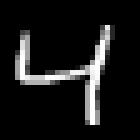
\includegraphics[width=0.1\textwidth]{Images/final/4/003_benign.jpg}
		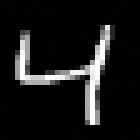
\includegraphics[width=0.1\textwidth]{Images/final/4/003_ben_L2_lambda=0.001_dist=0.13505950570106506_d2=0.13505950570106506.jpg}
		
\includegraphics[width=0.1\textwidth]{Images/final/4/003_ben_L2_lambda=0.01_dist=0.1562836468219757_d2=0.1562836468219757.jpg}
		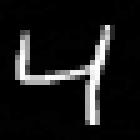
\includegraphics[width=0.1\textwidth]{Images/final/4/003_ben_L2_lambda=0.1_dist=0.16468484699726105_d2=0.16468484699726105.jpg}
		
\includegraphics[width=0.1\textwidth]{Images/final/4/003_adv_L2_lambda=1_dist=1.8425648212432861_d2=1.8425648212432861.jpg}
		
\includegraphics[width=0.1\textwidth]{Images/final/4/003_adv_L2_lambda=10_dist=1.8296877145767212_d2=1.8296877145767212.jpg}
		
\includegraphics[width=0.1\textwidth]{Images/final/4/003_adv_L2_lambda=100_dist=1.9413517713546753_d2=1.9413517713546753.jpg}
		
\includegraphics[width=0.1\textwidth]{Images/final/4/003_adv_L2_lambda=1000_dist=2.39263916015625_d2=2.39263916015625.jpg}
	\end{subfigure}
	\begin{subfigure}[b]{\textwidth}
        \centering
		
\includegraphics[width=0.1\textwidth]{Images/final/5/001_benign.jpg}
		
\includegraphics[width=0.1\textwidth]{Images/final/5/001_ben_L2_lambda=0.001_dist=0.14381442964076996_d2=0.14381442964076996.jpg}
		
\includegraphics[width=0.1\textwidth]{Images/final/5/001_ben_L2_lambda=0.01_dist=0.1451040655374527_d2=0.1451040655374527.jpg}
		
\includegraphics[width=0.1\textwidth]{Images/final/5/001_ben_L2_lambda=0.1_dist=0.16168451309204102_d2=0.16168451309204102.jpg}
		
\includegraphics[width=0.1\textwidth]{Images/final/5/001_adv_L2_lambda=1_dist=0.3215978443622589_d2=0.3215978443622589.jpg}
		
\includegraphics[width=0.1\textwidth]{Images/final/5/001_adv_L2_lambda=10_dist=3.3893277645111084_d2=3.3893277645111084.jpg}
		\includegraphics[width=0.1\textwidth]{Images/final/5/001_adv_L2_lambda=100_dist=3.7630810737609863_d2=3.7630810737609863.jpg}
		\includegraphics[width=0.1\textwidth]{Images/final/5/001_adv_L2_lambda=1000_dist=3.95320200920105_d2=3.95320200920105.jpg}
	\end{subfigure}
	\begin{subfigure}[b]{\textwidth}
        \centering
		\includegraphics[width=0.1\textwidth]{Images/final/6/014_benign.jpg}
		\includegraphics[width=0.1\textwidth]{Images/final/6/014_ben_L2_lambda=0.001_dist=0.15017886459827423_d2=0.15017886459827423.jpg}
		\includegraphics[width=0.1\textwidth]{Images/final/6/014_ben_L2_lambda=0.01_dist=0.15716511011123657_d2=0.15716511011123657.jpg}
		\includegraphics[width=0.1\textwidth]{Images/final/6/014_ben_L2_lambda=0.1_dist=0.13287559151649475_d2=0.13287559151649475.jpg}
		\includegraphics[width=0.1\textwidth]{Images/final/6/014_adv_L2_lambda=1_dist=2.4251952171325684_d2=2.4251952171325684.jpg}
		\includegraphics[width=0.1\textwidth]{Images/final/6/014_adv_L2_lambda=10_dist=2.5936362743377686_d2=2.5936362743377686.jpg}
		\includegraphics[width=0.1\textwidth]{Images/final/6/014_adv_L2_lambda=100_dist=2.5497589111328125_d2=2.5497589111328125.jpg}
		\includegraphics[width=0.1\textwidth]{Images/final/6/014_adv_L2_lambda=1000_dist=2.828904390335083_d2=2.828904390335083.jpg}
	\end{subfigure}
	\begin{subfigure}[b]{\textwidth}
        \centering
		\includegraphics[width=0.1\textwidth]{Images/final/7/038_benign.jpg}
		\includegraphics[width=0.1\textwidth]{Images/final/7/038_ben_L2_lambda=0.001_dist=0.13506628572940826_d2=0.13506628572940826.jpg}
		\includegraphics[width=0.1\textwidth]{Images/final/7/038_ben_L2_lambda=0.01_dist=0.1388508528470993_d2=0.1388508528470993.jpg}
		\includegraphics[width=0.1\textwidth]{Images/final/7/038_ben_L2_lambda=0.1_dist=0.14036525785923004_d2=0.14036525785923004.jpg}
		\includegraphics[width=0.1\textwidth]{Images/final/7/038_adv_L2_lambda=1_dist=2.7284634113311768_d2=2.7284634113311768.jpg}
		\includegraphics[width=0.1\textwidth]{Images/final/7/038_adv_L2_lambda=10_dist=2.872725486755371_d2=2.872725486755371.jpg}
		\includegraphics[width=0.1\textwidth]{Images/final/7/038_adv_L2_lambda=100_dist=2.918837070465088_d2=2.918837070465088.jpg}
		\includegraphics[width=0.1\textwidth]{Images/final/7/038_adv_L2_lambda=1000_dist=3.1405227184295654_d2=3.1405227184295654.jpg}
	\end{subfigure}
	\begin{subfigure}[b]{\textwidth}
        \centering
		\includegraphics[width=0.1\textwidth]{Images/final/8/082_benign.jpg}
		\includegraphics[width=0.1\textwidth]{Images/final/8/082_ben_L2_lambda=0.001_dist=0.1464889645576477_d2=0.1464889645576477.jpg}
		\includegraphics[width=0.1\textwidth]{Images/final/8/082_ben_L2_lambda=0.01_dist=0.15887826681137085_d2=0.15887826681137085.jpg}
		\includegraphics[width=0.1\textwidth]{Images/final/8/082_ben_L2_lambda=0.1_dist=0.12859991192817688_d2=0.12859991192817688.jpg}
		\includegraphics[width=0.1\textwidth]{Images/final/8/082_ben_L2_lambda=1_dist=0.15008991956710815_d2=0.15008991956710815.jpg}
		\includegraphics[width=0.1\textwidth]{Images/final/8/082_adv_L2_lambda=10_dist=2.7434496879577637_d2=2.7434496879577637.jpg}
		\includegraphics[width=0.1\textwidth]{Images/final/8/082_adv_L2_lambda=100_dist=3.0015370845794678_d2=3.0015370845794678.jpg}
		\includegraphics[width=0.1\textwidth]{Images/final/8/082_adv_L2_lambda=1000_dist=3.1302969455718994_d2=3.1302969455718994.jpg}
	\end{subfigure}
	\begin{subfigure}[b]{\textwidth}
        \centering
		\includegraphics[width=0.1\textwidth]{Images/final/9/084_benign.jpg}
		\includegraphics[width=0.1\textwidth]{Images/final/9/084_ben_L2_lambda=0.001_dist=0.13593007624149323_d2=0.13593007624149323.jpg}
		\includegraphics[width=0.1\textwidth]{Images/final/9/084_ben_L2_lambda=0.01_dist=0.14051811397075653_d2=0.14051811397075653.jpg}
		\includegraphics[width=0.1\textwidth]{Images/final/9/084_ben_L2_lambda=0.1_dist=0.14687930047512054_d2=0.14687930047512054.jpg}
		\includegraphics[width=0.1\textwidth]{Images/final/9/084_adv_L2_lambda=1_dist=1.0900646448135376_d2=1.0900646448135376.jpg}
		\includegraphics[width=0.1\textwidth]{Images/final/9/084_adv_L2_lambda=10_dist=1.3691350221633911_d2=1.3691350221633911.jpg}
		\includegraphics[width=0.1\textwidth]{Images/final/9/084_adv_L2_lambda=100_dist=1.546129822731018_d2=1.546129822731018.jpg}
		\includegraphics[width=0.1\textwidth]{Images/final/9/084_adv_L2_lambda=1000_dist=1.5453290939331055_d2=1.5453290939331055.jpg}
	\end{subfigure}
	\centering
	\caption{Vzorky generované CW útokem za použití metriky indukované $l_2$ normou; v řádku po řadě původní benigní vzorek, dále vzorky vygenerované s rostoucí hodnotou parametru $\lambda$}
	\label{cw_L2}
\end{figure}


Na Obrázku \ref{cw_L2} lze spatřit vzorky vygenerované CW útokem
za použití metriky indukované $l_2$ normou.
V každém z řádků je potom prvním obrázkem původní benigní vzorek.
Následující obrázky v řádku jsou pootom obrázky vygenerované CW útokem pro variabilní hodnotu parametru $\lambda$.
Tato hodnota parametru $\lambda$ je potom po řadě $10^{-3}$, $10^{-2}$, $10^{-1}$, $1$, $10$, $100$ a $1000$.
V takovémto formátu potom jsou prezentovány i další obrázky.

Z Obrázku \ref{cw_L2} si lze odnést jednoznačně potvrzení prezentované matematické intuice
ohledně volby parametru $\lambda$ v CW útoku, který spočívá v řešení (\ref{cw_in_results}).
Čím větší je totiž parametr $\lambda$,
tím menší důraz je kladen na minimalizaci metriky vizuální podobnosti mezi původním benigním vzorkem a generovaným vzorkem.
Proto s rostoucí hodnotou parametru $\lambda$ narůstá míra vizuálního poškození oproti původnímu obrázku.

\section{Adversariální útok za použití metriky indukované $l_1$ normou}

% L1
\begin{figure}
    \centering
	\begin{subfigure}[b]{\textwidth}
        \centering
		\includegraphics[width=0.1\textwidth]{Images/final/0/002_benign.jpg}
		\includegraphics[width=0.1\textwidth]{Images/final/0/002_ben_L1_lambda=0.001_dist=2.1123158931732178_d2=0.13503792881965637.jpg}
		\includegraphics[width=0.1\textwidth]{Images/final/0/002_ben_L1_lambda=0.01_dist=2.2541632652282715_d2=0.14029383659362793.jpg}
		\includegraphics[width=0.1\textwidth]{Images/final/0/002_ben_L1_lambda=0.1_dist=2.164498805999756_d2=0.13702493906021118.jpg}
		\includegraphics[width=0.1\textwidth]{Images/final/0/002_ben_L1_lambda=1_dist=2.2262306213378906_d2=0.13875721395015717.jpg}
		\includegraphics[width=0.1\textwidth]{Images/final/0/002_adv_L1_lambda=10_dist=27.19317626953125_d2=4.186177730560303.jpg}
		\includegraphics[width=0.1\textwidth]{Images/final/0/002_adv_L1_lambda=100_dist=30.345487594604492_d2=4.266388416290283.jpg}
		\includegraphics[width=0.1\textwidth]{Images/final/0/002_adv_L1_lambda=1000_dist=39.962013244628906_d2=4.580175399780273.jpg}
	\end{subfigure}
	\begin{subfigure}[b]{\textwidth}
        \centering
		\includegraphics[width=0.1\textwidth]{Images/final/1/004_benign.jpg}
		\includegraphics[width=0.1\textwidth]{Images/final/1/004_ben_L1_lambda=0.001_dist=2.3379104137420654_d2=0.14730338752269745.jpg}
		\includegraphics[width=0.1\textwidth]{Images/final/1/004_ben_L1_lambda=0.01_dist=2.6827871799468994_d2=0.1587119698524475.jpg}
		\includegraphics[width=0.1\textwidth]{Images/final/1/004_ben_L1_lambda=0.1_dist=2.671137809753418_d2=0.1585993617773056.jpg}
		\includegraphics[width=0.1\textwidth]{Images/final/1/004_ben_L1_lambda=1_dist=2.3518543243408203_d2=0.1481785923242569.jpg}
		\includegraphics[width=0.1\textwidth]{Images/final/1/004_adv_L1_lambda=10_dist=12.21181583404541_d2=1.7675739526748657.jpg}
		\includegraphics[width=0.1\textwidth]{Images/final/1/004_adv_L1_lambda=100_dist=13.533018112182617_d2=1.817665934562683.jpg}
		\includegraphics[width=0.1\textwidth]{Images/final/1/004_adv_L1_lambda=1000_dist=20.231225967407227_d2=2.2448954582214355.jpg}
	\end{subfigure}
	\begin{subfigure}[b]{\textwidth}
        \centering
		\includegraphics[width=0.1\textwidth]{Images/final/2/006_benign.jpg}
		\includegraphics[width=0.1\textwidth]{Images/final/2/006_ben_L1_lambda=0.001_dist=2.2423954010009766_d2=0.13853515684604645.jpg}
		\includegraphics[width=0.1\textwidth]{Images/final/2/006_ben_L1_lambda=0.01_dist=2.1699607372283936_d2=0.1371910721063614.jpg}
		\includegraphics[width=0.1\textwidth]{Images/final/2/006_ben_L1_lambda=0.1_dist=2.651066780090332_d2=0.1523362696170807.jpg}
		\includegraphics[width=0.1\textwidth]{Images/final/2/006_ben_L1_lambda=1_dist=2.4909517765045166_d2=0.14790132641792297.jpg}
		\includegraphics[width=0.1\textwidth]{Images/final/2/006_adv_L1_lambda=10_dist=17.9833984375_d2=2.5667717456817627.jpg}
		\includegraphics[width=0.1\textwidth]{Images/final/2/006_adv_L1_lambda=100_dist=20.346904754638672_d2=2.6776912212371826.jpg}
		\includegraphics[width=0.1\textwidth]{Images/final/2/006_adv_L1_lambda=1000_dist=28.94110870361328_d2=2.9921469688415527.jpg}
	\end{subfigure}
	\begin{subfigure}[b]{\textwidth}
        \centering
		\includegraphics[width=0.1\textwidth]{Images/final/3/008_benign.jpg}
		\includegraphics[width=0.1\textwidth]{Images/final/3/008_ben_L1_lambda=0.001_dist=2.1820151805877686_d2=0.13565431535243988.jpg}
		\includegraphics[width=0.1\textwidth]{Images/final/3/008_ben_L1_lambda=0.01_dist=2.4119343757629395_d2=0.1439496874809265.jpg}
		\includegraphics[width=0.1\textwidth]{Images/final/3/008_ben_L1_lambda=0.1_dist=2.2867329120635986_d2=0.1399593949317932.jpg}
		\includegraphics[width=0.1\textwidth]{Images/final/3/008_ben_L1_lambda=1_dist=2.1649885177612305_d2=0.13583070039749146.jpg}
		\includegraphics[width=0.1\textwidth]{Images/final/3/008_adv_L1_lambda=10_dist=27.574554443359375_d2=3.2078564167022705.jpg}
		\includegraphics[width=0.1\textwidth]{Images/final/3/008_adv_L1_lambda=100_dist=29.116031646728516_d2=3.192244291305542.jpg}
		\includegraphics[width=0.1\textwidth]{Images/final/3/008_adv_L1_lambda=1000_dist=29.945934295654297_d2=3.262796401977539.jpg}
	\end{subfigure}
	\begin{subfigure}[b]{\textwidth}
        \centering
		\includegraphics[width=0.1\textwidth]{Images/final/4/003_benign.jpg}
		\includegraphics[width=0.1\textwidth]{Images/final/4/003_ben_L1_lambda=0.001_dist=2.981707811355591_d2=0.16678394377231598.jpg}
		\includegraphics[width=0.1\textwidth]{Images/final/4/003_ben_L1_lambda=0.01_dist=2.4039759635925293_d2=0.1483311653137207.jpg}
		\includegraphics[width=0.1\textwidth]{Images/final/4/003_ben_L1_lambda=0.1_dist=2.8642685413360596_d2=0.1634032130241394.jpg}
		\includegraphics[width=0.1\textwidth]{Images/final/4/003_ben_L1_lambda=1_dist=2.610167980194092_d2=0.15477555990219116.jpg}
		\includegraphics[width=0.1\textwidth]{Images/final/4/003_adv_L1_lambda=10_dist=15.790398597717285_d2=2.1837830543518066.jpg}
		\includegraphics[width=0.1\textwidth]{Images/final/4/003_adv_L1_lambda=100_dist=23.057170867919922_d2=2.7984237670898438.jpg}
		\includegraphics[width=0.1\textwidth]{Images/final/4/003_adv_L1_lambda=1000_dist=20.822385787963867_d2=2.3107895851135254.jpg}
	\end{subfigure}
	\begin{subfigure}[b]{\textwidth}
        \centering
		\includegraphics[width=0.1\textwidth]{Images/final/5/001_benign.jpg}
		\includegraphics[width=0.1\textwidth]{Images/final/5/001_ben_L1_lambda=0.001_dist=2.3076510429382324_d2=0.14183330535888672.jpg}
		\includegraphics[width=0.1\textwidth]{Images/final/5/001_ben_L1_lambda=0.01_dist=2.5378406047821045_d2=0.15009833872318268.jpg}
		\includegraphics[width=0.1\textwidth]{Images/final/5/001_ben_L1_lambda=0.1_dist=2.410611152648926_d2=0.14579333364963531.jpg}
		\includegraphics[width=0.1\textwidth]{Images/final/5/001_ben_L1_lambda=1_dist=2.5475614070892334_d2=0.15072689950466156.jpg}
		\includegraphics[width=0.1\textwidth]{Images/final/5/001_adv_L1_lambda=10_dist=3.56191349029541_d2=0.5998944640159607.jpg}
		\includegraphics[width=0.1\textwidth]{Images/final/5/001_adv_L1_lambda=100_dist=33.78354263305664_d2=4.158044815063477.jpg}
		\includegraphics[width=0.1\textwidth]{Images/final/5/001_adv_L1_lambda=1000_dist=42.122066497802734_d2=4.326496601104736.jpg}
	\end{subfigure}
	\begin{subfigure}[b]{\textwidth}
        \centering
		\includegraphics[width=0.1\textwidth]{Images/final/6/014_benign.jpg}
		\includegraphics[width=0.1\textwidth]{Images/final/6/014_ben_L1_lambda=0.001_dist=2.1245415210723877_d2=0.13561014831066132.jpg}
		\includegraphics[width=0.1\textwidth]{Images/final/6/014_ben_L1_lambda=0.01_dist=2.361963987350464_d2=0.14437228441238403.jpg}
		\includegraphics[width=0.1\textwidth]{Images/final/6/014_ben_L1_lambda=0.1_dist=2.5869898796081543_d2=0.15171116590499878.jpg}
		\includegraphics[width=0.1\textwidth]{Images/final/6/014_ben_L1_lambda=1_dist=2.2592079639434814_d2=0.14099909365177155.jpg}
		\includegraphics[width=0.1\textwidth]{Images/final/6/014_adv_L1_lambda=10_dist=22.019609451293945_d2=2.975619077682495.jpg}
		\includegraphics[width=0.1\textwidth]{Images/final/6/014_adv_L1_lambda=100_dist=27.41433334350586_d2=3.1519129276275635.jpg}
		\includegraphics[width=0.1\textwidth]{Images/final/6/014_adv_L1_lambda=1000_dist=33.84744644165039_d2=3.2057480812072754.jpg}
	\end{subfigure}
	\begin{subfigure}[b]{\textwidth}
        \centering
		\includegraphics[width=0.1\textwidth]{Images/final/7/038_benign.jpg}
		\includegraphics[width=0.1\textwidth]{Images/final/7/038_ben_L1_lambda=0.001_dist=2.0468955039978027_d2=0.1336158961057663.jpg}
		\includegraphics[width=0.1\textwidth]{Images/final/7/038_ben_L1_lambda=0.01_dist=2.4102141857147217_d2=0.14693641662597656.jpg}
		\includegraphics[width=0.1\textwidth]{Images/final/7/038_ben_L1_lambda=0.1_dist=2.42751145362854_d2=0.14749430119991302.jpg}
		\includegraphics[width=0.1\textwidth]{Images/final/7/038_ben_L1_lambda=1_dist=2.2019050121307373_d2=0.1394798457622528.jpg}
		\includegraphics[width=0.1\textwidth]{Images/final/7/038_adv_L1_lambda=10_dist=29.234840393066406_d2=3.302190065383911.jpg}
		\includegraphics[width=0.1\textwidth]{Images/final/7/038_adv_L1_lambda=100_dist=31.231565475463867_d2=3.2983813285827637.jpg}
		\includegraphics[width=0.1\textwidth]{Images/final/7/038_adv_L1_lambda=1000_dist=36.032676696777344_d2=3.603574514389038.jpg}
	\end{subfigure}
	\begin{subfigure}[b]{\textwidth}
        \centering
		\includegraphics[width=0.1\textwidth]{Images/final/8/082_benign.jpg}
		\includegraphics[width=0.1\textwidth]{Images/final/8/082_ben_L1_lambda=0.001_dist=2.0222933292388916_d2=0.13158689439296722.jpg}
		\includegraphics[width=0.1\textwidth]{Images/final/8/082_ben_L1_lambda=0.01_dist=1.9499961137771606_d2=0.1292506903409958.jpg}
		\includegraphics[width=0.1\textwidth]{Images/final/8/082_ben_L1_lambda=0.1_dist=2.5400733947753906_d2=0.15101462602615356.jpg}
		\includegraphics[width=0.1\textwidth]{Images/final/8/082_ben_L1_lambda=1_dist=2.835761070251465_d2=0.15978097915649414.jpg}
		\includegraphics[width=0.1\textwidth]{Images/final/8/082_ben_L1_lambda=10_dist=1.8253750801086426_d2=0.12419386208057404.jpg}
		\includegraphics[width=0.1\textwidth]{Images/final/8/082_adv_L1_lambda=100_dist=25.795658111572266_d2=3.6265883445739746.jpg}
		\includegraphics[width=0.1\textwidth]{Images/final/8/082_adv_L1_lambda=1000_dist=33.083152770996094_d2=3.5952515602111816.jpg}
	\end{subfigure}
	\begin{subfigure}[b]{\textwidth}
        \centering
		\includegraphics[width=0.1\textwidth]{Images/final/9/084_benign.jpg}
		\includegraphics[width=0.1\textwidth]{Images/final/9/084_ben_L1_lambda=0.001_dist=2.362851858139038_d2=0.14393684267997742.jpg}
		\includegraphics[width=0.1\textwidth]{Images/final/9/084_ben_L1_lambda=0.01_dist=2.286245584487915_d2=0.14126403629779816.jpg}
		\includegraphics[width=0.1\textwidth]{Images/final/9/084_ben_L1_lambda=0.1_dist=2.4285104274749756_d2=0.1457786113023758.jpg}
		\includegraphics[width=0.1\textwidth]{Images/final/9/084_ben_L1_lambda=1_dist=2.4015541076660156_d2=0.1451183259487152.jpg}
		\includegraphics[width=0.1\textwidth]{Images/final/9/084_adv_L1_lambda=10_dist=8.838101387023926_d2=1.755147099494934.jpg}
		\includegraphics[width=0.1\textwidth]{Images/final/9/084_adv_L1_lambda=100_dist=12.764104843139648_d2=1.7609970569610596.jpg}
		\includegraphics[width=0.1\textwidth]{Images/final/9/084_adv_L1_lambda=1000_dist=13.054327011108398_d2=1.8567101955413818.jpg}
	\end{subfigure}
	\centering
	\caption{Vzorky generované CW útokem za použití metriky indukované $l_1$ normou; v řádku po řadě původní benigní vzorek, dále vzorky vygenerované s rostoucí hodnotou parametru $\lambda$}
	\label{cw_L1}
\end{figure}

Na Obrázku \ref{cw_L1} lze pak spatřit vzorky vygenerované CW útokem,
který používal metriku vizuální podobnosti indukovanou $l_1$ normou.
Na první pohled při srovnání s Obrázkem \ref{cw_L2} lze vidět,
že vzorky generované za použití metriky indukované $l_1$ normou
jsou poněkud kostrbatější.
Tak jinak, že artefakty v okolí číslic mají výrazně větší rozdíly v hodnotách dvou sousedních pixelů.

\section{Adversariální útok za použití metriky vizuální podobnosti DSSIM}

Podívejme se nyní na vzorky vygenerované CW útokem, ve kterém roli metriky vizuální podobnosti
hrála metrika vizuální podobnosti \emph{DSSIM}.
Předvedli jsme, že tato metrika sama o sobě je parametrizovaná velikostí výpočetního podokna.
Proto se věnujme různým velikostem výpočetního podokna zvlášť.

\subsection{Velikost výpočetního podokna 5}

% DSSIM-ws=5
\begin{figure}
    \centering
	\begin{subfigure}[b]{\textwidth}
        \centering
		\includegraphics[width=0.1\textwidth]{Images/final/0/002_benign.jpg}
		\includegraphics[width=0.1\textwidth]{Images/final/0/002_ben_DSSIM-ws=5_lambda=0.001_dist=0.012907654047012329_d2=0.25780388712882996.jpg}
		\includegraphics[width=0.1\textwidth]{Images/final/0/002_adv_DSSIM-ws=5_lambda=0.01_dist=0.1795159876346588_d2=8.1172456741333.jpg}
		\includegraphics[width=0.1\textwidth]{Images/final/0/002_adv_DSSIM-ws=5_lambda=0.1_dist=0.1948918104171753_d2=8.852614402770996.jpg}
		\includegraphics[width=0.1\textwidth]{Images/final/0/002_adv_DSSIM-ws=5_lambda=1_dist=0.19347989559173584_d2=9.060647010803223.jpg}
		\includegraphics[width=0.1\textwidth]{Images/final/0/002_adv_DSSIM-ws=5_lambda=10_dist=0.2138414978981018_d2=9.165953636169434.jpg}
		\includegraphics[width=0.1\textwidth]{Images/final/0/002_adv_DSSIM-ws=5_lambda=100_dist=0.19990432262420654_d2=8.26209831237793.jpg}
		\includegraphics[width=0.1\textwidth]{Images/final/0/002_adv_DSSIM-ws=5_lambda=1000_dist=0.22542142868041992_d2=9.986775398254395.jpg}
	\end{subfigure}
	\begin{subfigure}[b]{\textwidth}
        \centering
		\includegraphics[width=0.1\textwidth]{Images/final/1/004_benign.jpg}
		\includegraphics[width=0.1\textwidth]{Images/final/1/004_adv_DSSIM-ws=5_lambda=0.001_dist=0.20210552215576172_d2=5.204440593719482.jpg}
		\includegraphics[width=0.1\textwidth]{Images/final/1/004_adv_DSSIM-ws=5_lambda=0.01_dist=0.23129743337631226_d2=6.779479503631592.jpg}
		\includegraphics[width=0.1\textwidth]{Images/final/1/004_adv_DSSIM-ws=5_lambda=0.1_dist=0.23670092225074768_d2=6.842749118804932.jpg}
		\includegraphics[width=0.1\textwidth]{Images/final/1/004_adv_DSSIM-ws=5_lambda=1_dist=0.24890384078025818_d2=9.283989906311035.jpg}
		\includegraphics[width=0.1\textwidth]{Images/final/1/004_adv_DSSIM-ws=5_lambda=10_dist=0.26059892773628235_d2=10.350024223327637.jpg}
		\includegraphics[width=0.1\textwidth]{Images/final/1/004_adv_DSSIM-ws=5_lambda=100_dist=0.2678776979446411_d2=10.019732475280762.jpg}
		\includegraphics[width=0.1\textwidth]{Images/final/1/004_adv_DSSIM-ws=5_lambda=1000_dist=0.2762296497821808_d2=9.126455307006836.jpg}
	\end{subfigure}
	\begin{subfigure}[b]{\textwidth}
        \centering
		\includegraphics[width=0.1\textwidth]{Images/final/2/006_benign.jpg}
		\includegraphics[width=0.1\textwidth]{Images/final/2/006_ben_DSSIM-ws=5_lambda=0.001_dist=0.015439987182617188_d2=0.28457263112068176.jpg}
		\includegraphics[width=0.1\textwidth]{Images/final/2/006_adv_DSSIM-ws=5_lambda=0.01_dist=0.18845707178115845_d2=9.144709587097168.jpg}
		\includegraphics[width=0.1\textwidth]{Images/final/2/006_adv_DSSIM-ws=5_lambda=0.1_dist=0.1839909553527832_d2=8.517693519592285.jpg}
		\includegraphics[width=0.1\textwidth]{Images/final/2/006_adv_DSSIM-ws=5_lambda=1_dist=0.2086554765701294_d2=9.226920127868652.jpg}
		\includegraphics[width=0.1\textwidth]{Images/final/2/006_adv_DSSIM-ws=5_lambda=10_dist=0.20963367819786072_d2=8.942191123962402.jpg}
		\includegraphics[width=0.1\textwidth]{Images/final/2/006_adv_DSSIM-ws=5_lambda=100_dist=0.20310166478157043_d2=8.989212036132812.jpg}
		\includegraphics[width=0.1\textwidth]{Images/final/2/006_adv_DSSIM-ws=5_lambda=1000_dist=0.2108789086341858_d2=8.91487979888916.jpg}
	\end{subfigure}
	\begin{subfigure}[b]{\textwidth}
        \centering
		\includegraphics[width=0.1\textwidth]{Images/final/3/008_benign.jpg}
		\includegraphics[width=0.1\textwidth]{Images/final/3/008_ben_DSSIM-ws=5_lambda=0.001_dist=0.027407854795455933_d2=0.17754097282886505.jpg}
		\includegraphics[width=0.1\textwidth]{Images/final/3/008_adv_DSSIM-ws=5_lambda=0.01_dist=0.1511649191379547_d2=9.185309410095215.jpg}
		\includegraphics[width=0.1\textwidth]{Images/final/3/008_adv_DSSIM-ws=5_lambda=0.1_dist=0.1671978235244751_d2=9.506505012512207.jpg}
		\includegraphics[width=0.1\textwidth]{Images/final/3/008_adv_DSSIM-ws=5_lambda=1_dist=0.16220921277999878_d2=8.844636917114258.jpg}
		\includegraphics[width=0.1\textwidth]{Images/final/3/008_adv_DSSIM-ws=5_lambda=10_dist=0.17757141590118408_d2=9.711848258972168.jpg}
		\includegraphics[width=0.1\textwidth]{Images/final/3/008_adv_DSSIM-ws=5_lambda=100_dist=0.17280831933021545_d2=9.6594877243042.jpg}
		\includegraphics[width=0.1\textwidth]{Images/final/3/008_adv_DSSIM-ws=5_lambda=1000_dist=0.1959558129310608_d2=10.52166748046875.jpg}
	\end{subfigure}
	\begin{subfigure}[b]{\textwidth}
        \centering
		\includegraphics[width=0.1\textwidth]{Images/final/4/003_benign.jpg}
		\includegraphics[width=0.1\textwidth]{Images/final/4/003_adv_DSSIM-ws=5_lambda=0.001_dist=0.1294924020767212_d2=3.768853187561035.jpg}
		\includegraphics[width=0.1\textwidth]{Images/final/4/003_adv_DSSIM-ws=5_lambda=0.01_dist=0.13068458437919617_d2=2.879298210144043.jpg}
		\includegraphics[width=0.1\textwidth]{Images/final/4/003_adv_DSSIM-ws=5_lambda=0.1_dist=0.21812522411346436_d2=7.8325700759887695.jpg}
		\includegraphics[width=0.1\textwidth]{Images/final/4/003_adv_DSSIM-ws=5_lambda=1_dist=0.21592074632644653_d2=8.568694114685059.jpg}
		\includegraphics[width=0.1\textwidth]{Images/final/4/003_adv_DSSIM-ws=5_lambda=10_dist=0.22601446509361267_d2=7.854658603668213.jpg}
		\includegraphics[width=0.1\textwidth]{Images/final/4/003_adv_DSSIM-ws=5_lambda=100_dist=0.22503170371055603_d2=8.015763282775879.jpg}
		\includegraphics[width=0.1\textwidth]{Images/final/4/003_adv_DSSIM-ws=5_lambda=1000_dist=0.22725751996040344_d2=8.192279815673828.jpg}
	\end{subfigure}
	\begin{subfigure}[b]{\textwidth}
        \centering
		\includegraphics[width=0.1\textwidth]{Images/final/5/001_benign.jpg}
		\includegraphics[width=0.1\textwidth]{Images/final/5/001_adv_DSSIM-ws=5_lambda=0.001_dist=0.13633859157562256_d2=7.0264105796813965.jpg}
		\includegraphics[width=0.1\textwidth]{Images/final/5/001_adv_DSSIM-ws=5_lambda=0.01_dist=0.17612865567207336_d2=7.836599826812744.jpg}
		\includegraphics[width=0.1\textwidth]{Images/final/5/001_adv_DSSIM-ws=5_lambda=0.1_dist=0.2083093523979187_d2=9.700610160827637.jpg}
		\includegraphics[width=0.1\textwidth]{Images/final/5/001_adv_DSSIM-ws=5_lambda=1_dist=0.21543562412261963_d2=9.925210952758789.jpg}
		\includegraphics[width=0.1\textwidth]{Images/final/5/001_adv_DSSIM-ws=5_lambda=10_dist=0.2163827121257782_d2=9.466742515563965.jpg}
		\includegraphics[width=0.1\textwidth]{Images/final/5/001_adv_DSSIM-ws=5_lambda=100_dist=0.23258158564567566_d2=10.717977523803711.jpg}
		\includegraphics[width=0.1\textwidth]{Images/final/5/001_adv_DSSIM-ws=5_lambda=1000_dist=0.23164480924606323_d2=10.952765464782715.jpg}
	\end{subfigure}
	\begin{subfigure}[b]{\textwidth}
        \centering
		\includegraphics[width=0.1\textwidth]{Images/final/6/014_benign.jpg}
		\includegraphics[width=0.1\textwidth]{Images/final/6/014_ben_DSSIM-ws=5_lambda=0.001_dist=0.0901041328907013_d2=1.0241386890411377.jpg}
		\includegraphics[width=0.1\textwidth]{Images/final/6/014_adv_DSSIM-ws=5_lambda=0.01_dist=0.20872414112091064_d2=9.780447006225586.jpg}
		\includegraphics[width=0.1\textwidth]{Images/final/6/014_adv_DSSIM-ws=5_lambda=0.1_dist=0.23172414302825928_d2=9.859075546264648.jpg}
		\includegraphics[width=0.1\textwidth]{Images/final/6/014_adv_DSSIM-ws=5_lambda=1_dist=0.23727938532829285_d2=9.169720649719238.jpg}
		\includegraphics[width=0.1\textwidth]{Images/final/6/014_adv_DSSIM-ws=5_lambda=10_dist=0.23269423842430115_d2=9.417067527770996.jpg}
		\includegraphics[width=0.1\textwidth]{Images/final/6/014_adv_DSSIM-ws=5_lambda=100_dist=0.24606120586395264_d2=9.927529335021973.jpg}
		\includegraphics[width=0.1\textwidth]{Images/final/6/014_adv_DSSIM-ws=5_lambda=1000_dist=0.2311561107635498_d2=9.109362602233887.jpg}
	\end{subfigure}
	\begin{subfigure}[b]{\textwidth}
        \centering
		\includegraphics[width=0.1\textwidth]{Images/final/7/038_benign.jpg}
		\includegraphics[width=0.1\textwidth]{Images/final/7/038_ben_DSSIM-ws=5_lambda=0.001_dist=0.1831589937210083_d2=6.411322593688965.jpg}
		\includegraphics[width=0.1\textwidth]{Images/final/7/038_adv_DSSIM-ws=5_lambda=0.01_dist=0.1912754774093628_d2=8.928193092346191.jpg}
		\includegraphics[width=0.1\textwidth]{Images/final/7/038_adv_DSSIM-ws=5_lambda=0.1_dist=0.241008460521698_d2=9.046478271484375.jpg}
		\includegraphics[width=0.1\textwidth]{Images/final/7/038_adv_DSSIM-ws=5_lambda=1_dist=0.2372835874557495_d2=9.185465812683105.jpg}
		\includegraphics[width=0.1\textwidth]{Images/final/7/038_adv_DSSIM-ws=5_lambda=10_dist=0.2498740255832672_d2=9.531346321105957.jpg}
		\includegraphics[width=0.1\textwidth]{Images/final/7/038_adv_DSSIM-ws=5_lambda=100_dist=0.25761061906814575_d2=9.553542137145996.jpg}
		\includegraphics[width=0.1\textwidth]{Images/final/7/038_adv_DSSIM-ws=5_lambda=1000_dist=0.2655770182609558_d2=9.616020202636719.jpg}
	\end{subfigure}
	\begin{subfigure}[b]{\textwidth}
        \centering
		\includegraphics[width=0.1\textwidth]{Images/final/8/082_benign.jpg}
		\includegraphics[width=0.1\textwidth]{Images/final/8/082_ben_DSSIM-ws=5_lambda=0.001_dist=0.005824416875839233_d2=0.40162259340286255.jpg}
		\includegraphics[width=0.1\textwidth]{Images/final/8/082_adv_DSSIM-ws=5_lambda=0.01_dist=0.17005816102027893_d2=9.058201789855957.jpg}
		\includegraphics[width=0.1\textwidth]{Images/final/8/082_adv_DSSIM-ws=5_lambda=0.1_dist=0.18513870239257812_d2=9.558727264404297.jpg}
		\includegraphics[width=0.1\textwidth]{Images/final/8/082_adv_DSSIM-ws=5_lambda=1_dist=0.2054150104522705_d2=10.678581237792969.jpg}
		\includegraphics[width=0.1\textwidth]{Images/final/8/082_adv_DSSIM-ws=5_lambda=10_dist=0.21524208784103394_d2=10.966041564941406.jpg}
		\includegraphics[width=0.1\textwidth]{Images/final/8/082_adv_DSSIM-ws=5_lambda=100_dist=0.20919692516326904_d2=9.878133773803711.jpg}
		\includegraphics[width=0.1\textwidth]{Images/final/8/082_adv_DSSIM-ws=5_lambda=1000_dist=0.2026299238204956_d2=9.93602180480957.jpg}
	\end{subfigure}
	\begin{subfigure}[b]{\textwidth}
        \centering
		\includegraphics[width=0.1\textwidth]{Images/final/9/084_benign.jpg}
		\includegraphics[width=0.1\textwidth]{Images/final/9/084_ben_DSSIM-ws=5_lambda=0.001_dist=0.1539323627948761_d2=2.0178327560424805.jpg}
		\includegraphics[width=0.1\textwidth]{Images/final/9/084_adv_DSSIM-ws=5_lambda=0.01_dist=0.1953158974647522_d2=8.86357307434082.jpg}
		\includegraphics[width=0.1\textwidth]{Images/final/9/084_adv_DSSIM-ws=5_lambda=0.1_dist=0.20213571190834045_d2=8.9537353515625.jpg}
		\includegraphics[width=0.1\textwidth]{Images/final/9/084_adv_DSSIM-ws=5_lambda=1_dist=0.2150484323501587_d2=8.490336418151855.jpg}
		\includegraphics[width=0.1\textwidth]{Images/final/9/084_adv_DSSIM-ws=5_lambda=10_dist=0.218455970287323_d2=8.784497261047363.jpg}
		\includegraphics[width=0.1\textwidth]{Images/final/9/084_adv_DSSIM-ws=5_lambda=100_dist=0.21162065863609314_d2=9.035633087158203.jpg}
		\includegraphics[width=0.1\textwidth]{Images/final/9/084_adv_DSSIM-ws=5_lambda=1000_dist=0.22423532605171204_d2=9.380809783935547.jpg}
	\end{subfigure}
	\centering
	\caption{Vzorky generované CW útokem za použití metriky vizuální podobnosti DSSIM s velikostí výpočetního podokna 5; v řádku po řadě původní benigní vzorek, dále vzorky vygenerované s rostoucí hodnotou parametru $\lambda$}
	\label{cw_DSSIM-ws5}
\end{figure}

Tento komentář se bude věnovat jevu, který vyvstal pro DSSIM útok
s parametrem velikosti výpočetního podokna $5$.
Podle Obrázku \ref{cw_DSSIM-ws5}
bývá po tomto útoku okolí číslice silně znečištěno artefakty.
Kupodivu samotná číslice a její bezprostřední okolí je relativně nedotknuté.
Tento fenomén se vyskytl hlavně u volby velikosti výpočetního podokna $5$.
Vysvětlení zní jednoduše.
Neboť je původní benigní obrázek dál od číslice roven v každém pixelu nule,
pak SSIM index příslušných dvou podoken dál od číslice vychází konstantně skoro nula,
a to kvůli členu $\sigma_{x \tilde{x}}$ v čitateli ve výrazu v (\ref{ssimm_def}).
Není úplně nula díky konstantě $C_2$, která zde vystupuje kvůli dělení.
Ta je ovšem dostatečně malá, aby byla převážena druhým členem gradientu.

% \begin{figure}[h]
%     \centering
%     \includegraphics[width=0.2\textwidth]{Images/dssim.png}
%     \caption{Příklad vzorku vygenerovaného DSSIM útokem} \label{dssim_pic}
% \end{figure}

\subsection{Velikost výpočetního podokna 10}

% DSSIM-ws=10
\begin{figure}
    \centering
	\begin{subfigure}[b]{\textwidth}
        \centering
		\includegraphics[width=0.1\textwidth]{Images/final/0/002_benign.jpg}
		\includegraphics[width=0.1\textwidth]{Images/final/0/002_ben_DSSIM-ws=10_lambda=0.001_dist=7.164478302001953e-05_d2=0.1196574941277504.jpg}
		\includegraphics[width=0.1\textwidth]{Images/final/0/002_ben_DSSIM-ws=10_lambda=0.01_dist=6.490945816040039e-05_d2=0.11181505769491196.jpg}
		\includegraphics[width=0.1\textwidth]{Images/final/0/002_adv_DSSIM-ws=10_lambda=0.1_dist=0.09023252129554749_d2=4.325859069824219.jpg}
		\includegraphics[width=0.1\textwidth]{Images/final/0/002_adv_DSSIM-ws=10_lambda=1_dist=0.087883859872818_d2=4.236833572387695.jpg}
		\includegraphics[width=0.1\textwidth]{Images/final/0/002_adv_DSSIM-ws=10_lambda=10_dist=0.09423938393592834_d2=4.4223833084106445.jpg}
		\includegraphics[width=0.1\textwidth]{Images/final/0/002_adv_DSSIM-ws=10_lambda=100_dist=0.09321200847625732_d2=4.364864826202393.jpg}
		\includegraphics[width=0.1\textwidth]{Images/final/0/002_adv_DSSIM-ws=10_lambda=1000_dist=0.13410040736198425_d2=5.532363414764404.jpg}
	\end{subfigure}
	\begin{subfigure}[b]{\textwidth}
        \centering
		\includegraphics[width=0.1\textwidth]{Images/final/1/004_benign.jpg}
		\includegraphics[width=0.1\textwidth]{Images/final/1/004_ben_DSSIM-ws=10_lambda=0.001_dist=0.017471134662628174_d2=0.19093060493469238.jpg}
		\includegraphics[width=0.1\textwidth]{Images/final/1/004_adv_DSSIM-ws=10_lambda=0.01_dist=0.06740507483482361_d2=2.2929306030273438.jpg}
		\includegraphics[width=0.1\textwidth]{Images/final/1/004_adv_DSSIM-ws=10_lambda=0.1_dist=0.10999441146850586_d2=5.145431041717529.jpg}
		\includegraphics[width=0.1\textwidth]{Images/final/1/004_adv_DSSIM-ws=10_lambda=1_dist=0.12007474899291992_d2=5.114199638366699.jpg}
		\includegraphics[width=0.1\textwidth]{Images/final/1/004_adv_DSSIM-ws=10_lambda=10_dist=0.12638157606124878_d2=4.356586933135986.jpg}
		\includegraphics[width=0.1\textwidth]{Images/final/1/004_adv_DSSIM-ws=10_lambda=100_dist=0.1350964605808258_d2=5.028470516204834.jpg}
		\includegraphics[width=0.1\textwidth]{Images/final/1/004_adv_DSSIM-ws=10_lambda=1000_dist=0.1326221525669098_d2=5.161792755126953.jpg}
	\end{subfigure}
	\begin{subfigure}[b]{\textwidth}
        \centering
		\includegraphics[width=0.1\textwidth]{Images/final/2/006_benign.jpg}
		\includegraphics[width=0.1\textwidth]{Images/final/2/006_ben_DSSIM-ws=10_lambda=0.001_dist=0.002175360918045044_d2=0.25739526748657227.jpg}
		\includegraphics[width=0.1\textwidth]{Images/final/2/006_ben_DSSIM-ws=10_lambda=0.01_dist=0.0023291707038879395_d2=0.4006381928920746.jpg}
		\includegraphics[width=0.1\textwidth]{Images/final/2/006_adv_DSSIM-ws=10_lambda=0.1_dist=0.018177270889282227_d2=2.0069732666015625.jpg}
		\includegraphics[width=0.1\textwidth]{Images/final/2/006_adv_DSSIM-ws=10_lambda=1_dist=0.026419639587402344_d2=2.4049811363220215.jpg}
		\includegraphics[width=0.1\textwidth]{Images/final/2/006_adv_DSSIM-ws=10_lambda=10_dist=0.031520992517471313_d2=2.572556257247925.jpg}
		\includegraphics[width=0.1\textwidth]{Images/final/2/006_adv_DSSIM-ws=10_lambda=100_dist=0.033131688833236694_d2=2.678351879119873.jpg}
		\includegraphics[width=0.1\textwidth]{Images/final/2/006_adv_DSSIM-ws=10_lambda=1000_dist=0.04540678858757019_d2=3.215731620788574.jpg}
	\end{subfigure}
	\begin{subfigure}[b]{\textwidth}
        \centering
		\includegraphics[width=0.1\textwidth]{Images/final/3/008_benign.jpg}
		\includegraphics[width=0.1\textwidth]{Images/final/3/008_ben_DSSIM-ws=10_lambda=0.001_dist=0.0015662908554077148_d2=0.20423398911952972.jpg}
		\includegraphics[width=0.1\textwidth]{Images/final/3/008_ben_DSSIM-ws=10_lambda=0.01_dist=0.02069556713104248_d2=1.627138614654541.jpg}
		\includegraphics[width=0.1\textwidth]{Images/final/3/008_adv_DSSIM-ws=10_lambda=0.1_dist=0.049358636140823364_d2=2.785853385925293.jpg}
		\includegraphics[width=0.1\textwidth]{Images/final/3/008_adv_DSSIM-ws=10_lambda=1_dist=0.04892030358314514_d2=2.8331410884857178.jpg}
		\includegraphics[width=0.1\textwidth]{Images/final/3/008_adv_DSSIM-ws=10_lambda=10_dist=0.06899017095565796_d2=3.4474456310272217.jpg}
		\includegraphics[width=0.1\textwidth]{Images/final/3/008_adv_DSSIM-ws=10_lambda=100_dist=0.06778690218925476_d2=3.5352752208709717.jpg}
		\includegraphics[width=0.1\textwidth]{Images/final/3/008_adv_DSSIM-ws=10_lambda=1000_dist=0.0722944438457489_d2=3.744856595993042.jpg}
	\end{subfigure}
	\begin{subfigure}[b]{\textwidth}
        \centering
		\includegraphics[width=0.1\textwidth]{Images/final/4/003_benign.jpg}
		\includegraphics[width=0.1\textwidth]{Images/final/4/003_ben_DSSIM-ws=10_lambda=0.001_dist=0.024586230516433716_d2=0.26586347818374634.jpg}
		\includegraphics[width=0.1\textwidth]{Images/final/4/003_ben_DSSIM-ws=10_lambda=0.01_dist=0.007821112871170044_d2=0.26596349477767944.jpg}
		\includegraphics[width=0.1\textwidth]{Images/final/4/003_adv_DSSIM-ws=10_lambda=0.1_dist=0.07514217495918274_d2=1.7968941926956177.jpg}
		\includegraphics[width=0.1\textwidth]{Images/final/4/003_adv_DSSIM-ws=10_lambda=1_dist=0.07844454050064087_d2=2.122070550918579.jpg}
		\includegraphics[width=0.1\textwidth]{Images/final/4/003_adv_DSSIM-ws=10_lambda=10_dist=0.08278557658195496_d2=2.23720383644104.jpg}
		\includegraphics[width=0.1\textwidth]{Images/final/4/003_adv_DSSIM-ws=10_lambda=100_dist=0.10463014245033264_d2=3.0959529876708984.jpg}
		\includegraphics[width=0.1\textwidth]{Images/final/4/003_adv_DSSIM-ws=10_lambda=1000_dist=0.0930790901184082_d2=2.5392844676971436.jpg}
	\end{subfigure}
	\begin{subfigure}[b]{\textwidth}
        \centering
		\includegraphics[width=0.1\textwidth]{Images/final/5/001_benign.jpg}
		\includegraphics[width=0.1\textwidth]{Images/final/5/001_adv_DSSIM-ws=10_lambda=0.001_dist=0.0004194676876068115_d2=0.2766514718532562.jpg}
		\includegraphics[width=0.1\textwidth]{Images/final/5/001_adv_DSSIM-ws=10_lambda=0.01_dist=0.0011091232299804688_d2=0.46529316902160645.jpg}
		\includegraphics[width=0.1\textwidth]{Images/final/5/001_adv_DSSIM-ws=10_lambda=0.1_dist=0.00199735164642334_d2=0.6264770030975342.jpg}
		\includegraphics[width=0.1\textwidth]{Images/final/5/001_adv_DSSIM-ws=10_lambda=1_dist=0.08404785394668579_d2=3.7348978519439697.jpg}
		\includegraphics[width=0.1\textwidth]{Images/final/5/001_adv_DSSIM-ws=10_lambda=10_dist=0.10273027420043945_d2=4.203285217285156.jpg}
		\includegraphics[width=0.1\textwidth]{Images/final/5/001_adv_DSSIM-ws=10_lambda=100_dist=0.10273781418800354_d2=4.272779941558838.jpg}
		\includegraphics[width=0.1\textwidth]{Images/final/5/001_adv_DSSIM-ws=10_lambda=1000_dist=0.12482860684394836_d2=4.878007411956787.jpg}
	\end{subfigure}
	\begin{subfigure}[b]{\textwidth}
        \centering
		\includegraphics[width=0.1\textwidth]{Images/final/6/014_benign.jpg}
		\includegraphics[width=0.1\textwidth]{Images/final/6/014_ben_DSSIM-ws=10_lambda=0.001_dist=0.0028899013996124268_d2=0.23144745826721191.jpg}
		\includegraphics[width=0.1\textwidth]{Images/final/6/014_ben_DSSIM-ws=10_lambda=0.01_dist=0.005318164825439453_d2=0.9649099707603455.jpg}
		\includegraphics[width=0.1\textwidth]{Images/final/6/014_adv_DSSIM-ws=10_lambda=0.1_dist=0.0436931848526001_d2=2.6055681705474854.jpg}
		\includegraphics[width=0.1\textwidth]{Images/final/6/014_adv_DSSIM-ws=10_lambda=1_dist=0.044647812843322754_d2=2.7104287147521973.jpg}
		\includegraphics[width=0.1\textwidth]{Images/final/6/014_adv_DSSIM-ws=10_lambda=10_dist=0.05327048897743225_d2=2.9401633739471436.jpg}
		\includegraphics[width=0.1\textwidth]{Images/final/6/014_adv_DSSIM-ws=10_lambda=100_dist=0.055208444595336914_d2=3.0852527618408203.jpg}
		\includegraphics[width=0.1\textwidth]{Images/final/6/014_adv_DSSIM-ws=10_lambda=1000_dist=0.06357496976852417_d2=3.401062250137329.jpg}
	\end{subfigure}
	\begin{subfigure}[b]{\textwidth}
        \centering
		\includegraphics[width=0.1\textwidth]{Images/final/7/038_benign.jpg}
		\includegraphics[width=0.1\textwidth]{Images/final/7/038_ben_DSSIM-ws=10_lambda=0.001_dist=0.003778219223022461_d2=0.18980194628238678.jpg}
		\includegraphics[width=0.1\textwidth]{Images/final/7/038_adv_DSSIM-ws=10_lambda=0.01_dist=0.024834126234054565_d2=2.495858669281006.jpg}
		\includegraphics[width=0.1\textwidth]{Images/final/7/038_adv_DSSIM-ws=10_lambda=0.1_dist=0.05835437774658203_d2=2.9837288856506348.jpg}
		\includegraphics[width=0.1\textwidth]{Images/final/7/038_adv_DSSIM-ws=10_lambda=1_dist=0.06087943911552429_d2=3.158695936203003.jpg}
		\includegraphics[width=0.1\textwidth]{Images/final/7/038_adv_DSSIM-ws=10_lambda=10_dist=0.05943310260772705_d2=3.026944160461426.jpg}
		\includegraphics[width=0.1\textwidth]{Images/final/7/038_adv_DSSIM-ws=10_lambda=100_dist=0.08003544807434082_d2=3.451349973678589.jpg}
		\includegraphics[width=0.1\textwidth]{Images/final/7/038_adv_DSSIM-ws=10_lambda=1000_dist=0.09739726781845093_d2=3.9389090538024902.jpg}
	\end{subfigure}
	\begin{subfigure}[b]{\textwidth}
        \centering
		\includegraphics[width=0.1\textwidth]{Images/final/8/082_benign.jpg}
		\includegraphics[width=0.1\textwidth]{Images/final/8/082_ben_DSSIM-ws=10_lambda=0.001_dist=0.00010055303573608398_d2=0.12951572239398956.jpg}
		\includegraphics[width=0.1\textwidth]{Images/final/8/082_ben_DSSIM-ws=10_lambda=0.01_dist=0.00012806057929992676_d2=0.14641311764717102.jpg}
		\includegraphics[width=0.1\textwidth]{Images/final/8/082_ben_DSSIM-ws=10_lambda=0.1_dist=0.007791578769683838_d2=0.34231916069984436.jpg}
		\includegraphics[width=0.1\textwidth]{Images/final/8/082_adv_DSSIM-ws=10_lambda=1_dist=0.09383758902549744_d2=4.385049819946289.jpg}
		\includegraphics[width=0.1\textwidth]{Images/final/8/082_adv_DSSIM-ws=10_lambda=10_dist=0.09834852814674377_d2=5.586298942565918.jpg}
		\includegraphics[width=0.1\textwidth]{Images/final/8/082_adv_DSSIM-ws=10_lambda=100_dist=0.10602039098739624_d2=5.25981330871582.jpg}
		\includegraphics[width=0.1\textwidth]{Images/final/8/082_adv_DSSIM-ws=10_lambda=1000_dist=0.12272489070892334_d2=6.162153244018555.jpg}
	\end{subfigure}
	\begin{subfigure}[b]{\textwidth}
        \centering
		\includegraphics[width=0.1\textwidth]{Images/final/9/084_benign.jpg}
		\includegraphics[width=0.1\textwidth]{Images/final/9/084_ben_DSSIM-ws=10_lambda=0.001_dist=0.00419771671295166_d2=0.20414355397224426.jpg}
		\includegraphics[width=0.1\textwidth]{Images/final/9/084_adv_DSSIM-ws=10_lambda=0.01_dist=0.00973406434059143_d2=1.317968726158142.jpg}
		\includegraphics[width=0.1\textwidth]{Images/final/9/084_adv_DSSIM-ws=10_lambda=0.1_dist=0.013548970222473145_d2=1.3641301393508911.jpg}
		\includegraphics[width=0.1\textwidth]{Images/final/9/084_adv_DSSIM-ws=10_lambda=1_dist=0.016219109296798706_d2=1.554163932800293.jpg}
		\includegraphics[width=0.1\textwidth]{Images/final/9/084_adv_DSSIM-ws=10_lambda=10_dist=0.028433382511138916_d2=1.816705346107483.jpg}
		\includegraphics[width=0.1\textwidth]{Images/final/9/084_adv_DSSIM-ws=10_lambda=100_dist=0.029317259788513184_d2=1.8892021179199219.jpg}
		\includegraphics[width=0.1\textwidth]{Images/final/9/084_adv_DSSIM-ws=10_lambda=1000_dist=0.03318724036216736_d2=2.132869005203247.jpg}
	\end{subfigure}
	\centering
	\caption{Vzorky generované CW útokem za použití metriky vizuální podobnosti DSSIM s velikostí výpočetního podokna 10; v řádku po řadě původní benigní vzorek, dále vzorky vygenerované s rostoucí hodnotou parametru $\lambda$}
	\label{cw_DSSIM-ws10}
\end{figure}

V Obrázku \ref{cw_DSSIM-ws10} lze potom nahlédnout na vzorky vygenerované CW útokem za použití metriky vizuální podobnosti
DSSIM s parametrem velikosti výpočetního podokna $10$.
Lze vidět, že tyto obrázky jsou mnohem uhlazenější, než obrázky vygenerované za použití metriky DSSIM s velikostí podokna $5$.

\subsection{Velikost výpočetního podokna 20}

% DSSIM-ws=20
\begin{figure}
    \centering
	\begin{subfigure}[b]{\textwidth}
        \centering
		\includegraphics[width=0.1\textwidth]{Images/final/0/002_benign.jpg}
		\includegraphics[width=0.1\textwidth]{Images/final/0/002_ben_DSSIM-ws=20_lambda=0.001_dist=0.0002536475658416748_d2=0.2619484066963196.jpg}
		\includegraphics[width=0.1\textwidth]{Images/final/0/002_adv_DSSIM-ws=20_lambda=0.01_dist=0.05227923393249512_d2=3.586812973022461.jpg}
		\includegraphics[width=0.1\textwidth]{Images/final/0/002_adv_DSSIM-ws=20_lambda=0.1_dist=0.06815275549888611_d2=4.063248634338379.jpg}
		\includegraphics[width=0.1\textwidth]{Images/final/0/002_adv_DSSIM-ws=20_lambda=1_dist=0.0890173614025116_d2=4.722400188446045.jpg}
		\includegraphics[width=0.1\textwidth]{Images/final/0/002_adv_DSSIM-ws=20_lambda=10_dist=0.06364130973815918_d2=3.9932949542999268.jpg}
		\includegraphics[width=0.1\textwidth]{Images/final/0/002_adv_DSSIM-ws=20_lambda=100_dist=0.0853385329246521_d2=4.742477893829346.jpg}
		\includegraphics[width=0.1\textwidth]{Images/final/0/002_adv_DSSIM-ws=20_lambda=1000_dist=0.0804310142993927_d2=4.547694206237793.jpg}
	\end{subfigure}
	\begin{subfigure}[b]{\textwidth}
        \centering
		\includegraphics[width=0.1\textwidth]{Images/final/1/004_benign.jpg}
		\includegraphics[width=0.1\textwidth]{Images/final/1/004_ben_DSSIM-ws=20_lambda=0.001_dist=0.0007454156875610352_d2=0.2676762044429779.jpg}
		\includegraphics[width=0.1\textwidth]{Images/final/1/004_adv_DSSIM-ws=20_lambda=0.01_dist=0.012452870607376099_d2=1.4461766481399536.jpg}
		\includegraphics[width=0.1\textwidth]{Images/final/1/004_adv_DSSIM-ws=20_lambda=0.1_dist=0.01756301522254944_d2=1.7218313217163086.jpg}
		\includegraphics[width=0.1\textwidth]{Images/final/1/004_adv_DSSIM-ws=20_lambda=1_dist=0.017003566026687622_d2=1.7202914953231812.jpg}
		\includegraphics[width=0.1\textwidth]{Images/final/1/004_adv_DSSIM-ws=20_lambda=10_dist=0.0216372013092041_d2=1.992215633392334.jpg}
		\includegraphics[width=0.1\textwidth]{Images/final/1/004_adv_DSSIM-ws=20_lambda=100_dist=0.027839094400405884_d2=2.202068328857422.jpg}
		\includegraphics[width=0.1\textwidth]{Images/final/1/004_adv_DSSIM-ws=20_lambda=1000_dist=0.03605261445045471_d2=2.4640982151031494.jpg}
	\end{subfigure}
	\begin{subfigure}[b]{\textwidth}
        \centering
		\includegraphics[width=0.1\textwidth]{Images/final/2/006_benign.jpg}
		\includegraphics[width=0.1\textwidth]{Images/final/2/006_ben_DSSIM-ws=20_lambda=0.001_dist=7.274746894836426e-05_d2=0.12097795307636261.jpg}
		\includegraphics[width=0.1\textwidth]{Images/final/2/006_adv_DSSIM-ws=20_lambda=0.01_dist=0.013227671384811401_d2=1.9472262859344482.jpg}
		\includegraphics[width=0.1\textwidth]{Images/final/2/006_adv_DSSIM-ws=20_lambda=0.1_dist=0.01752626895904541_d2=2.248422145843506.jpg}
		\includegraphics[width=0.1\textwidth]{Images/final/2/006_adv_DSSIM-ws=20_lambda=1_dist=0.016385912895202637_d2=2.1885485649108887.jpg}
		\includegraphics[width=0.1\textwidth]{Images/final/2/006_adv_DSSIM-ws=20_lambda=10_dist=0.01826539635658264_d2=2.300792694091797.jpg}
		\includegraphics[width=0.1\textwidth]{Images/final/2/006_adv_DSSIM-ws=20_lambda=100_dist=0.023336023092269897_d2=2.6493306159973145.jpg}
		\includegraphics[width=0.1\textwidth]{Images/final/2/006_adv_DSSIM-ws=20_lambda=1000_dist=0.030865520238876343_d2=3.1120152473449707.jpg}
	\end{subfigure}
	\begin{subfigure}[b]{\textwidth}
        \centering
		\includegraphics[width=0.1\textwidth]{Images/final/3/008_benign.jpg}
		\includegraphics[width=0.1\textwidth]{Images/final/3/008_ben_DSSIM-ws=20_lambda=0.001_dist=5.3495168685913086e-05_d2=0.11688616871833801.jpg}
		\includegraphics[width=0.1\textwidth]{Images/final/3/008_ben_DSSIM-ws=20_lambda=0.01_dist=0.02042633295059204_d2=2.405867576599121.jpg}
		\includegraphics[width=0.1\textwidth]{Images/final/3/008_adv_DSSIM-ws=20_lambda=0.1_dist=0.028211981058120728_d2=2.823099374771118.jpg}
		\includegraphics[width=0.1\textwidth]{Images/final/3/008_adv_DSSIM-ws=20_lambda=1_dist=0.0243205726146698_d2=2.6722304821014404.jpg}
		\includegraphics[width=0.1\textwidth]{Images/final/3/008_adv_DSSIM-ws=20_lambda=10_dist=0.03502354025840759_d2=3.238971710205078.jpg}
		\includegraphics[width=0.1\textwidth]{Images/final/3/008_adv_DSSIM-ws=20_lambda=100_dist=0.031292229890823364_d2=3.046889066696167.jpg}
		\includegraphics[width=0.1\textwidth]{Images/final/3/008_adv_DSSIM-ws=20_lambda=1000_dist=0.03934502601623535_d2=3.4120032787323.jpg}
	\end{subfigure}
	\begin{subfigure}[b]{\textwidth}
        \centering
		\includegraphics[width=0.1\textwidth]{Images/final/4/003_benign.jpg}
		\includegraphics[width=0.1\textwidth]{Images/final/4/003_ben_DSSIM-ws=20_lambda=0.001_dist=0.00010576844215393066_d2=0.1138145700097084.jpg}
		\includegraphics[width=0.1\textwidth]{Images/final/4/003_adv_DSSIM-ws=20_lambda=0.01_dist=0.019063591957092285_d2=1.7591419219970703.jpg}
		\includegraphics[width=0.1\textwidth]{Images/final/4/003_adv_DSSIM-ws=20_lambda=0.1_dist=0.029934555292129517_d2=2.279686450958252.jpg}
		\includegraphics[width=0.1\textwidth]{Images/final/4/003_adv_DSSIM-ws=20_lambda=1_dist=0.02082541584968567_d2=1.8923890590667725.jpg}
		\includegraphics[width=0.1\textwidth]{Images/final/4/003_adv_DSSIM-ws=20_lambda=10_dist=0.028116434812545776_d2=2.1299054622650146.jpg}
		\includegraphics[width=0.1\textwidth]{Images/final/4/003_adv_DSSIM-ws=20_lambda=100_dist=0.035455524921417236_d2=2.406920909881592.jpg}
		\includegraphics[width=0.1\textwidth]{Images/final/4/003_adv_DSSIM-ws=20_lambda=1000_dist=0.048074185848236084_d2=2.8166542053222656.jpg}
	\end{subfigure}
	\begin{subfigure}[b]{\textwidth}
        \centering
		\includegraphics[width=0.1\textwidth]{Images/final/5/001_benign.jpg}
		\includegraphics[width=0.1\textwidth]{Images/final/5/001_adv_DSSIM-ws=20_lambda=0.001_dist=0.00028893351554870605_d2=0.2715969681739807.jpg}
		\includegraphics[width=0.1\textwidth]{Images/final/5/001_adv_DSSIM-ws=20_lambda=0.01_dist=0.0005349516868591309_d2=0.38237038254737854.jpg}
		\includegraphics[width=0.1\textwidth]{Images/final/5/001_adv_DSSIM-ws=20_lambda=0.1_dist=0.0008066296577453613_d2=0.4562113583087921.jpg}
		\includegraphics[width=0.1\textwidth]{Images/final/5/001_adv_DSSIM-ws=20_lambda=1_dist=0.05349186062812805_d2=3.563622236251831.jpg}
		\includegraphics[width=0.1\textwidth]{Images/final/5/001_adv_DSSIM-ws=20_lambda=10_dist=0.0727250874042511_d2=4.283256530761719.jpg}
		\includegraphics[width=0.1\textwidth]{Images/final/5/001_adv_DSSIM-ws=20_lambda=100_dist=0.08257243037223816_d2=4.570023059844971.jpg}
		\includegraphics[width=0.1\textwidth]{Images/final/5/001_adv_DSSIM-ws=20_lambda=1000_dist=0.1032477617263794_d2=5.008537292480469.jpg}
	\end{subfigure}
	\begin{subfigure}[b]{\textwidth}
        \centering
		\includegraphics[width=0.1\textwidth]{Images/final/6/014_benign.jpg}
		\includegraphics[width=0.1\textwidth]{Images/final/6/014_ben_DSSIM-ws=20_lambda=0.001_dist=0.00023999810218811035_d2=0.25963878631591797.jpg}
		\includegraphics[width=0.1\textwidth]{Images/final/6/014_adv_DSSIM-ws=20_lambda=0.01_dist=0.020062893629074097_d2=2.282846689224243.jpg}
		\includegraphics[width=0.1\textwidth]{Images/final/6/014_adv_DSSIM-ws=20_lambda=0.1_dist=0.024713784456253052_d2=2.6404504776000977.jpg}
		\includegraphics[width=0.1\textwidth]{Images/final/6/014_adv_DSSIM-ws=20_lambda=1_dist=0.026410281658172607_d2=2.7093589305877686.jpg}
		\includegraphics[width=0.1\textwidth]{Images/final/6/014_adv_DSSIM-ws=20_lambda=10_dist=0.0341305136680603_d2=3.0598204135894775.jpg}
		\includegraphics[width=0.1\textwidth]{Images/final/6/014_adv_DSSIM-ws=20_lambda=100_dist=0.03563907742500305_d2=3.1036391258239746.jpg}
		\includegraphics[width=0.1\textwidth]{Images/final/6/014_adv_DSSIM-ws=20_lambda=1000_dist=0.05019453167915344_d2=3.7255473136901855.jpg}
	\end{subfigure}
	\begin{subfigure}[b]{\textwidth}
        \centering
		\includegraphics[width=0.1\textwidth]{Images/final/7/038_benign.jpg}
		\includegraphics[width=0.1\textwidth]{Images/final/7/038_ben_DSSIM-ws=20_lambda=0.001_dist=9.146332740783691e-05_d2=0.1178731620311737.jpg}
		\includegraphics[width=0.1\textwidth]{Images/final/7/038_adv_DSSIM-ws=20_lambda=0.01_dist=0.013421237468719482_d2=1.954052209854126.jpg}
		\includegraphics[width=0.1\textwidth]{Images/final/7/038_adv_DSSIM-ws=20_lambda=0.1_dist=0.03714904189109802_d2=2.848768711090088.jpg}
		\includegraphics[width=0.1\textwidth]{Images/final/7/038_adv_DSSIM-ws=20_lambda=1_dist=0.0450916588306427_d2=3.2110743522644043.jpg}
		\includegraphics[width=0.1\textwidth]{Images/final/7/038_adv_DSSIM-ws=20_lambda=10_dist=0.04645398259162903_d2=3.1877267360687256.jpg}
		\includegraphics[width=0.1\textwidth]{Images/final/7/038_adv_DSSIM-ws=20_lambda=100_dist=0.04811674356460571_d2=3.2384021282196045.jpg}
		\includegraphics[width=0.1\textwidth]{Images/final/7/038_adv_DSSIM-ws=20_lambda=1000_dist=0.06724599003791809_d2=3.8644540309906006.jpg}
	\end{subfigure}
	\begin{subfigure}[b]{\textwidth}
        \centering
		\includegraphics[width=0.1\textwidth]{Images/final/8/082_benign.jpg}
		\includegraphics[width=0.1\textwidth]{Images/final/8/082_ben_DSSIM-ws=20_lambda=0.001_dist=0.0003052353858947754_d2=0.2603950798511505.jpg}
		\includegraphics[width=0.1\textwidth]{Images/final/8/082_ben_DSSIM-ws=20_lambda=0.01_dist=0.0003399848937988281_d2=0.262408047914505.jpg}
		\includegraphics[width=0.1\textwidth]{Images/final/8/082_adv_DSSIM-ws=20_lambda=0.1_dist=0.032473206520080566_d2=2.756079912185669.jpg}
		\includegraphics[width=0.1\textwidth]{Images/final/8/082_adv_DSSIM-ws=20_lambda=1_dist=0.03551363945007324_d2=2.9440250396728516.jpg}
		\includegraphics[width=0.1\textwidth]{Images/final/8/082_adv_DSSIM-ws=20_lambda=10_dist=0.050937652587890625_d2=3.4137957096099854.jpg}
		\includegraphics[width=0.1\textwidth]{Images/final/8/082_adv_DSSIM-ws=20_lambda=100_dist=0.05226027965545654_d2=3.610316276550293.jpg}
		\includegraphics[width=0.1\textwidth]{Images/final/8/082_adv_DSSIM-ws=20_lambda=1000_dist=0.0578746497631073_d2=3.809668779373169.jpg}
	\end{subfigure}
	\begin{subfigure}[b]{\textwidth}
        \centering
		\includegraphics[width=0.1\textwidth]{Images/final/9/084_benign.jpg}
		\includegraphics[width=0.1\textwidth]{Images/final/9/084_ben_DSSIM-ws=20_lambda=0.001_dist=0.00024375319480895996_d2=0.2611492872238159.jpg}
		\includegraphics[width=0.1\textwidth]{Images/final/9/084_adv_DSSIM-ws=20_lambda=0.01_dist=0.0039331912994384766_d2=1.051363468170166.jpg}
		\includegraphics[width=0.1\textwidth]{Images/final/9/084_adv_DSSIM-ws=20_lambda=0.1_dist=0.005749255418777466_d2=1.2325890064239502.jpg}
		\includegraphics[width=0.1\textwidth]{Images/final/9/084_adv_DSSIM-ws=20_lambda=1_dist=0.008408814668655396_d2=1.5102806091308594.jpg}
		\includegraphics[width=0.1\textwidth]{Images/final/9/084_adv_DSSIM-ws=20_lambda=10_dist=0.009465336799621582_d2=1.6464368104934692.jpg}
		\includegraphics[width=0.1\textwidth]{Images/final/9/084_adv_DSSIM-ws=20_lambda=100_dist=0.011113911867141724_d2=1.7896323204040527.jpg}
		\includegraphics[width=0.1\textwidth]{Images/final/9/084_adv_DSSIM-ws=20_lambda=1000_dist=0.011532217264175415_d2=1.7933346033096313.jpg}
	\end{subfigure}
	\centering
	\caption{Vzorky generované CW útokem za použití metriky vizuální podobnosti DSSIM s velikostí výpočetního podokna 20; v řádku po řadě původní benigní vzorek, dále vzorky vygenerované s rostoucí hodnotou parametru $\lambda$}
	\label{cw_DSSIM-ws20}
\end{figure}

V Obrázku \ref{cw_DSSIM-ws20} vidíme vzorky vygenerované CW útokem za použití metriky vizuální podobnosti
DSSIM s parametrem velikosti výpočetního podokna $20$.
Je patrné, že tyto obrázky jsou velice podobné těm,
jež jsou vygenerované za použití metriky DSSIM s velikostí podokna $10$.


\subsection{Velikost výpočetního podokna jako velikost celého obrázku}

% DSSIM-ws=28
\begin{figure}
    \centering
	\begin{subfigure}[b]{\textwidth}
        \centering
		\includegraphics[width=0.1\textwidth]{Images/final/0/002_benign.jpg}
		\includegraphics[width=0.1\textwidth]{Images/final/0/002_ben_DSSIM-ws=28_lambda=0.001_dist=0.0006527602672576904_d2=0.2597068250179291.jpg}
		\includegraphics[width=0.1\textwidth]{Images/final/0/002_ben_DSSIM-ws=28_lambda=0.01_dist=0.041407614946365356_d2=3.6191041469573975.jpg}
		\includegraphics[width=0.1\textwidth]{Images/final/0/002_adv_DSSIM-ws=28_lambda=0.1_dist=0.04590708017349243_d2=3.772212505340576.jpg}
		\includegraphics[width=0.1\textwidth]{Images/final/0/002_adv_DSSIM-ws=28_lambda=1_dist=0.05505719780921936_d2=4.110447883605957.jpg}
		\includegraphics[width=0.1\textwidth]{Images/final/0/002_adv_DSSIM-ws=28_lambda=10_dist=0.06139412522315979_d2=4.339127063751221.jpg}
		\includegraphics[width=0.1\textwidth]{Images/final/0/002_adv_DSSIM-ws=28_lambda=100_dist=0.06363588571548462_d2=4.417396068572998.jpg}
		\includegraphics[width=0.1\textwidth]{Images/final/0/002_adv_DSSIM-ws=28_lambda=1000_dist=0.07012525200843811_d2=4.609143257141113.jpg}
	\end{subfigure}
	\begin{subfigure}[b]{\textwidth}
        \centering
		\includegraphics[width=0.1\textwidth]{Images/final/1/004_benign.jpg}
		\includegraphics[width=0.1\textwidth]{Images/final/1/004_ben_DSSIM-ws=28_lambda=0.001_dist=7.051229476928711e-05_d2=0.09435642510652542.jpg}
		\includegraphics[width=0.1\textwidth]{Images/final/1/004_adv_DSSIM-ws=28_lambda=0.01_dist=0.0073160529136657715_d2=1.1654866933822632.jpg}
		\includegraphics[width=0.1\textwidth]{Images/final/1/004_adv_DSSIM-ws=28_lambda=0.1_dist=0.01363179087638855_d2=1.5549908876419067.jpg}
		\includegraphics[width=0.1\textwidth]{Images/final/1/004_adv_DSSIM-ws=28_lambda=1_dist=0.01316174864768982_d2=1.5603022575378418.jpg}
		\includegraphics[width=0.1\textwidth]{Images/final/1/004_adv_DSSIM-ws=28_lambda=10_dist=0.026003897190093994_d2=2.113497734069824.jpg}
		\includegraphics[width=0.1\textwidth]{Images/final/1/004_adv_DSSIM-ws=28_lambda=100_dist=0.02598714828491211_d2=2.1596240997314453.jpg}
		\includegraphics[width=0.1\textwidth]{Images/final/1/004_adv_DSSIM-ws=28_lambda=1000_dist=0.03694593906402588_d2=2.533818483352661.jpg}
	\end{subfigure}
	\begin{subfigure}[b]{\textwidth}
        \centering
		\includegraphics[width=0.1\textwidth]{Images/final/2/006_benign.jpg}
		\includegraphics[width=0.1\textwidth]{Images/final/2/006_ben_DSSIM-ws=28_lambda=0.001_dist=0.00010123848915100098_d2=0.1404988318681717.jpg}
		\includegraphics[width=0.1\textwidth]{Images/final/2/006_adv_DSSIM-ws=28_lambda=0.01_dist=0.012032747268676758_d2=1.8962154388427734.jpg}
		\includegraphics[width=0.1\textwidth]{Images/final/2/006_adv_DSSIM-ws=28_lambda=0.1_dist=0.01553162932395935_d2=2.141655206680298.jpg}
		\includegraphics[width=0.1\textwidth]{Images/final/2/006_adv_DSSIM-ws=28_lambda=1_dist=0.018947452306747437_d2=2.345529556274414.jpg}
		\includegraphics[width=0.1\textwidth]{Images/final/2/006_adv_DSSIM-ws=28_lambda=10_dist=0.022246092557907104_d2=2.5183136463165283.jpg}
		\includegraphics[width=0.1\textwidth]{Images/final/2/006_adv_DSSIM-ws=28_lambda=100_dist=0.026773184537887573_d2=2.765101909637451.jpg}
		\includegraphics[width=0.1\textwidth]{Images/final/2/006_adv_DSSIM-ws=28_lambda=1000_dist=0.03136235475540161_d2=2.9739797115325928.jpg}
	\end{subfigure}
	\begin{subfigure}[b]{\textwidth}
        \centering
		\includegraphics[width=0.1\textwidth]{Images/final/3/008_benign.jpg}
		\includegraphics[width=0.1\textwidth]{Images/final/3/008_ben_DSSIM-ws=28_lambda=0.001_dist=0.0004795193672180176_d2=0.25358501076698303.jpg}
		\includegraphics[width=0.1\textwidth]{Images/final/3/008_adv_DSSIM-ws=28_lambda=0.01_dist=0.018101096153259277_d2=2.54963755607605.jpg}
		\includegraphics[width=0.1\textwidth]{Images/final/3/008_adv_DSSIM-ws=28_lambda=0.1_dist=0.020111531019210815_d2=2.6727077960968018.jpg}
		\includegraphics[width=0.1\textwidth]{Images/final/3/008_adv_DSSIM-ws=28_lambda=1_dist=0.022642463445663452_d2=2.8139758110046387.jpg}
		\includegraphics[width=0.1\textwidth]{Images/final/3/008_adv_DSSIM-ws=28_lambda=10_dist=0.02468252182006836_d2=2.938100814819336.jpg}
		\includegraphics[width=0.1\textwidth]{Images/final/3/008_adv_DSSIM-ws=28_lambda=100_dist=0.025828152894973755_d2=3.023090124130249.jpg}
		\includegraphics[width=0.1\textwidth]{Images/final/3/008_adv_DSSIM-ws=28_lambda=1000_dist=0.03609591722488403_d2=3.511007785797119.jpg}
	\end{subfigure}
	\begin{subfigure}[b]{\textwidth}
        \centering
		\includegraphics[width=0.1\textwidth]{Images/final/4/003_benign.jpg}
		\includegraphics[width=0.1\textwidth]{Images/final/4/003_ben_DSSIM-ws=28_lambda=0.001_dist=0.00012534856796264648_d2=0.12401768565177917.jpg}
		\includegraphics[width=0.1\textwidth]{Images/final/4/003_adv_DSSIM-ws=28_lambda=0.01_dist=0.014248698949813843_d2=1.6364364624023438.jpg}
		\includegraphics[width=0.1\textwidth]{Images/final/4/003_adv_DSSIM-ws=28_lambda=0.1_dist=0.026106446981430054_d2=2.1877503395080566.jpg}
		\includegraphics[width=0.1\textwidth]{Images/final/4/003_adv_DSSIM-ws=28_lambda=1_dist=0.02153158187866211_d2=1.9933834075927734.jpg}
		\includegraphics[width=0.1\textwidth]{Images/final/4/003_adv_DSSIM-ws=28_lambda=10_dist=0.029590904712677002_d2=2.2752604484558105.jpg}
		\includegraphics[width=0.1\textwidth]{Images/final/4/003_adv_DSSIM-ws=28_lambda=100_dist=0.03629648685455322_d2=2.513145923614502.jpg}
		\includegraphics[width=0.1\textwidth]{Images/final/4/003_adv_DSSIM-ws=28_lambda=1000_dist=0.03464081883430481_d2=2.489288091659546.jpg}
	\end{subfigure}
	\begin{subfigure}[b]{\textwidth}
        \centering
		\includegraphics[width=0.1\textwidth]{Images/final/5/001_benign.jpg}
		\includegraphics[width=0.1\textwidth]{Images/final/5/001_adv_DSSIM-ws=28_lambda=0.001_dist=0.0009191930294036865_d2=0.34530267119407654.jpg}
		\includegraphics[width=0.1\textwidth]{Images/final/5/001_adv_DSSIM-ws=28_lambda=0.01_dist=0.0011218786239624023_d2=0.45758673548698425.jpg}
		\includegraphics[width=0.1\textwidth]{Images/final/5/001_adv_DSSIM-ws=28_lambda=0.1_dist=0.001177072525024414_d2=0.5635843873023987.jpg}
		\includegraphics[width=0.1\textwidth]{Images/final/5/001_adv_DSSIM-ws=28_lambda=1_dist=0.049429893493652344_d2=3.6456172466278076.jpg}
		\includegraphics[width=0.1\textwidth]{Images/final/5/001_adv_DSSIM-ws=28_lambda=10_dist=0.06304094195365906_d2=4.077995300292969.jpg}
		\includegraphics[width=0.1\textwidth]{Images/final/5/001_adv_DSSIM-ws=28_lambda=100_dist=0.07135656476020813_d2=4.322898864746094.jpg}
		\includegraphics[width=0.1\textwidth]{Images/final/5/001_adv_DSSIM-ws=28_lambda=1000_dist=0.07862269878387451_d2=4.500265121459961.jpg}
	\end{subfigure}
	\begin{subfigure}[b]{\textwidth}
        \centering
		\includegraphics[width=0.1\textwidth]{Images/final/6/014_benign.jpg}
		\includegraphics[width=0.1\textwidth]{Images/final/6/014_ben_DSSIM-ws=28_lambda=0.001_dist=7.259845733642578e-05_d2=0.11978789418935776.jpg}
		\includegraphics[width=0.1\textwidth]{Images/final/6/014_ben_DSSIM-ws=28_lambda=0.01_dist=0.009091168642044067_d2=1.6406724452972412.jpg}
		\includegraphics[width=0.1\textwidth]{Images/final/6/014_adv_DSSIM-ws=28_lambda=0.1_dist=0.018837273120880127_d2=2.2993242740631104.jpg}
		\includegraphics[width=0.1\textwidth]{Images/final/6/014_adv_DSSIM-ws=28_lambda=1_dist=0.021842241287231445_d2=2.453716993331909.jpg}
		\includegraphics[width=0.1\textwidth]{Images/final/6/014_adv_DSSIM-ws=28_lambda=10_dist=0.02902156114578247_d2=2.8137245178222656.jpg}
		\includegraphics[width=0.1\textwidth]{Images/final/6/014_adv_DSSIM-ws=28_lambda=100_dist=0.03589361906051636_d2=3.118530035018921.jpg}
		\includegraphics[width=0.1\textwidth]{Images/final/6/014_adv_DSSIM-ws=28_lambda=1000_dist=0.036865800619125366_d2=3.1457228660583496.jpg}
	\end{subfigure}
	\begin{subfigure}[b]{\textwidth}
        \centering
		\includegraphics[width=0.1\textwidth]{Images/final/7/038_benign.jpg}
		\includegraphics[width=0.1\textwidth]{Images/final/7/038_ben_DSSIM-ws=28_lambda=0.001_dist=0.00012105703353881836_d2=0.1295614242553711.jpg}
		\includegraphics[width=0.1\textwidth]{Images/final/7/038_adv_DSSIM-ws=28_lambda=0.01_dist=0.017879962921142578_d2=2.0136446952819824.jpg}
		\includegraphics[width=0.1\textwidth]{Images/final/7/038_adv_DSSIM-ws=28_lambda=0.1_dist=0.033293455839157104_d2=2.6896750926971436.jpg}
		\includegraphics[width=0.1\textwidth]{Images/final/7/038_adv_DSSIM-ws=28_lambda=1_dist=0.04566633701324463_d2=3.0668554306030273.jpg}
		\includegraphics[width=0.1\textwidth]{Images/final/7/038_adv_DSSIM-ws=28_lambda=10_dist=0.04543134570121765_d2=3.096625328063965.jpg}
		\includegraphics[width=0.1\textwidth]{Images/final/7/038_adv_DSSIM-ws=28_lambda=100_dist=0.061637431383132935_d2=3.5399670600891113.jpg}
		\includegraphics[width=0.1\textwidth]{Images/final/7/038_adv_DSSIM-ws=28_lambda=1000_dist=0.06797045469284058_d2=3.644491672515869.jpg}
	\end{subfigure}
	\begin{subfigure}[b]{\textwidth}
        \centering
		\includegraphics[width=0.1\textwidth]{Images/final/8/082_benign.jpg}
		\includegraphics[width=0.1\textwidth]{Images/final/8/082_ben_DSSIM-ws=28_lambda=0.001_dist=0.0009506642818450928_d2=0.26098692417144775.jpg}
		\includegraphics[width=0.1\textwidth]{Images/final/8/082_ben_DSSIM-ws=28_lambda=0.01_dist=0.00011157989501953125_d2=0.1376025378704071.jpg}
		\includegraphics[width=0.1\textwidth]{Images/final/8/082_ben_DSSIM-ws=28_lambda=0.1_dist=0.001003265380859375_d2=0.26215821504592896.jpg}
		\includegraphics[width=0.1\textwidth]{Images/final/8/082_adv_DSSIM-ws=28_lambda=1_dist=0.031706303358078_d2=2.874894618988037.jpg}
		\includegraphics[width=0.1\textwidth]{Images/final/8/082_adv_DSSIM-ws=28_lambda=10_dist=0.03915989398956299_d2=3.176405191421509.jpg}
		\includegraphics[width=0.1\textwidth]{Images/final/8/082_adv_DSSIM-ws=28_lambda=100_dist=0.048934370279312134_d2=3.4788928031921387.jpg}
		\includegraphics[width=0.1\textwidth]{Images/final/8/082_adv_DSSIM-ws=28_lambda=1000_dist=0.05626785755157471_d2=3.752417802810669.jpg}
	\end{subfigure}
	\begin{subfigure}[b]{\textwidth}
        \centering
		\includegraphics[width=0.1\textwidth]{Images/final/9/084_benign.jpg}
		\includegraphics[width=0.1\textwidth]{Images/final/9/084_ben_DSSIM-ws=28_lambda=0.001_dist=0.00010079145431518555_d2=0.1375729739665985.jpg}
		\includegraphics[width=0.1\textwidth]{Images/final/9/084_adv_DSSIM-ws=28_lambda=0.01_dist=0.004255950450897217_d2=1.1294628381729126.jpg}
		\includegraphics[width=0.1\textwidth]{Images/final/9/084_adv_DSSIM-ws=28_lambda=0.1_dist=0.006579577922821045_d2=1.3868383169174194.jpg}
		\includegraphics[width=0.1\textwidth]{Images/final/9/084_adv_DSSIM-ws=28_lambda=1_dist=0.006243288516998291_d2=1.3543237447738647.jpg}
		\includegraphics[width=0.1\textwidth]{Images/final/9/084_adv_DSSIM-ws=28_lambda=10_dist=0.010649830102920532_d2=1.7357609272003174.jpg}
		\includegraphics[width=0.1\textwidth]{Images/final/9/084_adv_DSSIM-ws=28_lambda=100_dist=0.012982308864593506_d2=1.91720449924469.jpg}
		\includegraphics[width=0.1\textwidth]{Images/final/9/084_adv_DSSIM-ws=28_lambda=1000_dist=0.014223664999008179_d2=2.018277883529663.jpg}
	\end{subfigure}
	\centering
	\caption{Vzorky generované CW útokem za použití metriky vizuální podobnosti DSSIM bez omezení velikosti výpočetního podokna; v řádku po řadě původní benigní vzorek, dále vzorky vygenerované s rostoucí hodnotou parametru $\lambda$}
	\label{cw_DSSIM-ws28}
\end{figure}

Na Obrázku \ref{cw_DSSIM-ws28} lze spatřit vzorky vygenerované CW útokem za použití metriky vizuální podobnosti
DSSIM s neomezeným parametrem velikosti výpočetního podokna, resp. s velikostí $28$, jež je velikostí obázků.
Obdobně jako v předchozím případě jsou tyto obrázky velice podobné těm,
jež jsou vygenerované za použití metriky DSSIM s velikostí podokna $10$,
a tedy i za použití metriky DSSIM s velikostí výpočetního podokna $20$.

\section{Adversariální útok za použití aproximace Wassersteinovy vzdálenosti}

Podíváme-li se po řadě na Obrázky \ref{cw_WassersteinAproximation-reg5}, \ref{cw_WassersteinAproximation-reg10}
a \ref{cw_WassersteinAproximation-reg15},
kde jsou zobrazeny vzorky vygenerované CW útokem za použití aproximace Wassersteinovy vzdálenosti
s hodnotami regularizačního parametru $\xi$ po řadě $5$, $10$ a $15$,
uvidíme, že tyto vzorky jsou velice odlišné od vzorků předchozích,
a to obzvlášť pro hodnotu regularizace $5$.
Obrázky, které vznikly CW útokem za použití této metriky, jsou totiž jakoby rozmazané.
S rostoucím regularizačním parametrem $\xi$ potom tento efekt mizí
a jeví se na obrázcích již povědomé artefakty v okolí číslice.

% \subsection{Hodnota regularizace 5}

% WassersteinAproximation-reg=5
\begin{figure}
    \centering
	\begin{subfigure}[b]{\textwidth}
        \centering
		\includegraphics[width=0.1\textwidth]{Images/final/0/002_benign.jpg}
		\includegraphics[width=0.1\textwidth]{Images/final/0/002_ben_WassersteinAproximation-reg=5_lambda=0.001_dist=0.8862981796264648_d2=6.621276378631592.jpg}
		\includegraphics[width=0.1\textwidth]{Images/final/0/002_ben_WassersteinAproximation-reg=5_lambda=0.01_dist=0.8844916820526123_d2=6.604877948760986.jpg}
		\includegraphics[width=0.1\textwidth]{Images/final/0/002_adv_WassersteinAproximation-reg=5_lambda=0.1_dist=1.746572494506836_d2=9.347614288330078.jpg}
		\includegraphics[width=0.1\textwidth]{Images/final/0/002_adv_WassersteinAproximation-reg=5_lambda=1_dist=1.7554618120193481_d2=9.780027389526367.jpg}
		\includegraphics[width=0.1\textwidth]{Images/final/0/002_adv_WassersteinAproximation-reg=5_lambda=10_dist=1.6617238521575928_d2=9.297603607177734.jpg}
		\includegraphics[width=0.1\textwidth]{Images/final/0/002_adv_WassersteinAproximation-reg=5_lambda=100_dist=1.9210896492004395_d2=10.047322273254395.jpg}
		\includegraphics[width=0.1\textwidth]{Images/final/0/002_adv_WassersteinAproximation-reg=5_lambda=1000_dist=2.0439541339874268_d2=10.062275886535645.jpg}
	\end{subfigure}
	\begin{subfigure}[b]{\textwidth}
        \centering
		\includegraphics[width=0.1\textwidth]{Images/final/1/004_benign.jpg}
		\includegraphics[width=0.1\textwidth]{Images/final/1/004_adv_WassersteinAproximation-reg=5_lambda=0.001_dist=1.6001088619232178_d2=7.229477405548096.jpg}
		\includegraphics[width=0.1\textwidth]{Images/final/1/004_adv_WassersteinAproximation-reg=5_lambda=0.01_dist=1.8065619468688965_d2=7.638077259063721.jpg}
		\includegraphics[width=0.1\textwidth]{Images/final/1/004_adv_WassersteinAproximation-reg=5_lambda=0.1_dist=1.7932322025299072_d2=7.659536838531494.jpg}
		\includegraphics[width=0.1\textwidth]{Images/final/1/004_adv_WassersteinAproximation-reg=5_lambda=1_dist=1.8347406387329102_d2=7.810190677642822.jpg}
		\includegraphics[width=0.1\textwidth]{Images/final/1/004_adv_WassersteinAproximation-reg=5_lambda=10_dist=1.8884750604629517_d2=7.846939563751221.jpg}
		\includegraphics[width=0.1\textwidth]{Images/final/1/004_adv_WassersteinAproximation-reg=5_lambda=100_dist=1.7712972164154053_d2=7.6636433601379395.jpg}
		\includegraphics[width=0.1\textwidth]{Images/final/1/004_adv_WassersteinAproximation-reg=5_lambda=1000_dist=2.0329620838165283_d2=7.960882663726807.jpg}
	\end{subfigure}
	\begin{subfigure}[b]{\textwidth}
        \centering
		\includegraphics[width=0.1\textwidth]{Images/final/2/006_benign.jpg}
		\includegraphics[width=0.1\textwidth]{Images/final/2/006_ben_WassersteinAproximation-reg=5_lambda=0.001_dist=0.7207291722297668_d2=6.495874404907227.jpg}
		\includegraphics[width=0.1\textwidth]{Images/final/2/006_ben_WassersteinAproximation-reg=5_lambda=0.01_dist=0.7455974817276001_d2=6.6258039474487305.jpg}
		\includegraphics[width=0.1\textwidth]{Images/final/2/006_adv_WassersteinAproximation-reg=5_lambda=0.1_dist=0.9346767663955688_d2=7.651573657989502.jpg}
		\includegraphics[width=0.1\textwidth]{Images/final/2/006_adv_WassersteinAproximation-reg=5_lambda=1_dist=1.01240074634552_d2=8.008554458618164.jpg}
		\includegraphics[width=0.1\textwidth]{Images/final/2/006_adv_WassersteinAproximation-reg=5_lambda=10_dist=1.1604641675949097_d2=8.32709789276123.jpg}
		\includegraphics[width=0.1\textwidth]{Images/final/2/006_adv_WassersteinAproximation-reg=5_lambda=100_dist=1.2171125411987305_d2=8.265971183776855.jpg}
		\includegraphics[width=0.1\textwidth]{Images/final/2/006_adv_WassersteinAproximation-reg=5_lambda=1000_dist=1.3288006782531738_d2=8.623159408569336.jpg}
	\end{subfigure}
	\begin{subfigure}[b]{\textwidth}
        \centering
		\includegraphics[width=0.1\textwidth]{Images/final/3/008_benign.jpg}
		\includegraphics[width=0.1\textwidth]{Images/final/3/008_ben_WassersteinAproximation-reg=5_lambda=0.001_dist=0.7064793109893799_d2=5.797385215759277.jpg}
		\includegraphics[width=0.1\textwidth]{Images/final/3/008_ben_WassersteinAproximation-reg=5_lambda=0.01_dist=0.7255828976631165_d2=5.761415004730225.jpg}
		\includegraphics[width=0.1\textwidth]{Images/final/3/008_adv_WassersteinAproximation-reg=5_lambda=0.1_dist=0.883672833442688_d2=7.01281213760376.jpg}
		\includegraphics[width=0.1\textwidth]{Images/final/3/008_adv_WassersteinAproximation-reg=5_lambda=1_dist=0.9370800256729126_d2=7.2437334060668945.jpg}
		\includegraphics[width=0.1\textwidth]{Images/final/3/008_adv_WassersteinAproximation-reg=5_lambda=10_dist=1.028261661529541_d2=7.445345401763916.jpg}
		\includegraphics[width=0.1\textwidth]{Images/final/3/008_adv_WassersteinAproximation-reg=5_lambda=100_dist=1.0912973880767822_d2=7.880997657775879.jpg}
		\includegraphics[width=0.1\textwidth]{Images/final/3/008_adv_WassersteinAproximation-reg=5_lambda=1000_dist=1.0974570512771606_d2=7.845635414123535.jpg}
	\end{subfigure}
	\begin{subfigure}[b]{\textwidth}
        \centering
		\includegraphics[width=0.1\textwidth]{Images/final/4/003_benign.jpg}
		\includegraphics[width=0.1\textwidth]{Images/final/4/003_ben_WassersteinAproximation-reg=5_lambda=0.001_dist=1.152281641960144_d2=8.504473686218262.jpg}
		\includegraphics[width=0.1\textwidth]{Images/final/4/003_ben_WassersteinAproximation-reg=5_lambda=0.01_dist=1.0886719226837158_d2=8.41270637512207.jpg}
		\includegraphics[width=0.1\textwidth]{Images/final/4/003_adv_WassersteinAproximation-reg=5_lambda=0.1_dist=1.504589557647705_d2=9.654913902282715.jpg}
		\includegraphics[width=0.1\textwidth]{Images/final/4/003_adv_WassersteinAproximation-reg=5_lambda=1_dist=1.707051157951355_d2=9.938911437988281.jpg}
		\includegraphics[width=0.1\textwidth]{Images/final/4/003_adv_WassersteinAproximation-reg=5_lambda=10_dist=1.8592612743377686_d2=9.99897575378418.jpg}
		\includegraphics[width=0.1\textwidth]{Images/final/4/003_adv_WassersteinAproximation-reg=5_lambda=100_dist=1.9510226249694824_d2=10.389008522033691.jpg}
		\includegraphics[width=0.1\textwidth]{Images/final/4/003_adv_WassersteinAproximation-reg=5_lambda=1000_dist=1.8023929595947266_d2=9.980759620666504.jpg}
	\end{subfigure}
	\begin{subfigure}[b]{\textwidth}
        \centering
		\includegraphics[width=0.1\textwidth]{Images/final/5/001_benign.jpg}
		\includegraphics[width=0.1\textwidth]{Images/final/5/001_adv_WassersteinAproximation-reg=5_lambda=0.001_dist=0.974415123462677_d2=6.935202121734619.jpg}
		\includegraphics[width=0.1\textwidth]{Images/final/5/001_adv_WassersteinAproximation-reg=5_lambda=0.01_dist=0.9394680261611938_d2=6.760026931762695.jpg}
		\includegraphics[width=0.1\textwidth]{Images/final/5/001_adv_WassersteinAproximation-reg=5_lambda=0.1_dist=0.9472461938858032_d2=6.899412155151367.jpg}
		\includegraphics[width=0.1\textwidth]{Images/final/5/001_adv_WassersteinAproximation-reg=5_lambda=1_dist=1.218666434288025_d2=8.18005084991455.jpg}
		\includegraphics[width=0.1\textwidth]{Images/final/5/001_adv_WassersteinAproximation-reg=5_lambda=10_dist=1.3873517513275146_d2=8.578278541564941.jpg}
		\includegraphics[width=0.1\textwidth]{Images/final/5/001_adv_WassersteinAproximation-reg=5_lambda=100_dist=1.522538661956787_d2=9.003381729125977.jpg}
		\includegraphics[width=0.1\textwidth]{Images/final/5/001_adv_WassersteinAproximation-reg=5_lambda=1000_dist=1.5393439531326294_d2=9.149836540222168.jpg}
	\end{subfigure}
	\begin{subfigure}[b]{\textwidth}
        \centering
		\includegraphics[width=0.1\textwidth]{Images/final/6/014_benign.jpg}
		\includegraphics[width=0.1\textwidth]{Images/final/6/014_ben_WassersteinAproximation-reg=5_lambda=0.001_dist=0.7040831446647644_d2=6.098762512207031.jpg}
		\includegraphics[width=0.1\textwidth]{Images/final/6/014_ben_WassersteinAproximation-reg=5_lambda=0.01_dist=0.7758547067642212_d2=6.474674224853516.jpg}
		\includegraphics[width=0.1\textwidth]{Images/final/6/014_adv_WassersteinAproximation-reg=5_lambda=0.1_dist=1.098243236541748_d2=7.602115631103516.jpg}
		\includegraphics[width=0.1\textwidth]{Images/final/6/014_adv_WassersteinAproximation-reg=5_lambda=1_dist=1.166723370552063_d2=7.857276916503906.jpg}
		\includegraphics[width=0.1\textwidth]{Images/final/6/014_adv_WassersteinAproximation-reg=5_lambda=10_dist=1.3166545629501343_d2=8.06698226928711.jpg}
		\includegraphics[width=0.1\textwidth]{Images/final/6/014_adv_WassersteinAproximation-reg=5_lambda=100_dist=1.3633860349655151_d2=8.223560333251953.jpg}
		\includegraphics[width=0.1\textwidth]{Images/final/6/014_adv_WassersteinAproximation-reg=5_lambda=1000_dist=1.5184831619262695_d2=8.504654884338379.jpg}
	\end{subfigure}
	\begin{subfigure}[b]{\textwidth}
        \centering
		\includegraphics[width=0.1\textwidth]{Images/final/7/038_benign.jpg}
		\includegraphics[width=0.1\textwidth]{Images/final/7/038_ben_WassersteinAproximation-reg=5_lambda=0.001_dist=1.0781508684158325_d2=7.453847408294678.jpg}
		\includegraphics[width=0.1\textwidth]{Images/final/7/038_ben_WassersteinAproximation-reg=5_lambda=0.01_dist=1.1558363437652588_d2=7.546934127807617.jpg}
		\includegraphics[width=0.1\textwidth]{Images/final/7/038_adv_WassersteinAproximation-reg=5_lambda=0.1_dist=1.3628909587860107_d2=8.825139999389648.jpg}
		\includegraphics[width=0.1\textwidth]{Images/final/7/038_adv_WassersteinAproximation-reg=5_lambda=1_dist=1.6203213930130005_d2=9.559967041015625.jpg}
		\includegraphics[width=0.1\textwidth]{Images/final/7/038_adv_WassersteinAproximation-reg=5_lambda=10_dist=1.711950421333313_d2=9.672384262084961.jpg}
		\includegraphics[width=0.1\textwidth]{Images/final/7/038_adv_WassersteinAproximation-reg=5_lambda=100_dist=1.852337121963501_d2=10.029085159301758.jpg}
		\includegraphics[width=0.1\textwidth]{Images/final/7/038_adv_WassersteinAproximation-reg=5_lambda=1000_dist=1.8840830326080322_d2=10.007537841796875.jpg}
	\end{subfigure}
	\begin{subfigure}[b]{\textwidth}
        \centering
		\includegraphics[width=0.1\textwidth]{Images/final/8/082_benign.jpg}
		\includegraphics[width=0.1\textwidth]{Images/final/8/082_ben_WassersteinAproximation-reg=5_lambda=0.001_dist=0.9412094354629517_d2=7.188952922821045.jpg}
		\includegraphics[width=0.1\textwidth]{Images/final/8/082_ben_WassersteinAproximation-reg=5_lambda=0.01_dist=0.9253320097923279_d2=7.168346881866455.jpg}
		\includegraphics[width=0.1\textwidth]{Images/final/8/082_ben_WassersteinAproximation-reg=5_lambda=0.1_dist=0.8753965497016907_d2=6.975978851318359.jpg}
		\includegraphics[width=0.1\textwidth]{Images/final/8/082_adv_WassersteinAproximation-reg=5_lambda=1_dist=1.2502835988998413_d2=8.090779304504395.jpg}
		\includegraphics[width=0.1\textwidth]{Images/final/8/082_adv_WassersteinAproximation-reg=5_lambda=10_dist=1.2026729583740234_d2=8.05639934539795.jpg}
		\includegraphics[width=0.1\textwidth]{Images/final/8/082_adv_WassersteinAproximation-reg=5_lambda=100_dist=1.4140923023223877_d2=8.620211601257324.jpg}
		\includegraphics[width=0.1\textwidth]{Images/final/8/082_adv_WassersteinAproximation-reg=5_lambda=1000_dist=1.4863154888153076_d2=8.523412704467773.jpg}
	\end{subfigure}
	\begin{subfigure}[b]{\textwidth}
        \centering
		\includegraphics[width=0.1\textwidth]{Images/final/9/084_benign.jpg}
		\includegraphics[width=0.1\textwidth]{Images/final/9/084_ben_WassersteinAproximation-reg=5_lambda=0.001_dist=0.8400753736495972_d2=6.549287796020508.jpg}
		\includegraphics[width=0.1\textwidth]{Images/final/9/084_ben_WassersteinAproximation-reg=5_lambda=0.01_dist=0.8164393901824951_d2=6.4759321212768555.jpg}
		\includegraphics[width=0.1\textwidth]{Images/final/9/084_adv_WassersteinAproximation-reg=5_lambda=0.1_dist=0.8751378655433655_d2=6.777065753936768.jpg}
		\includegraphics[width=0.1\textwidth]{Images/final/9/084_adv_WassersteinAproximation-reg=5_lambda=1_dist=0.927515983581543_d2=6.75361442565918.jpg}
		\includegraphics[width=0.1\textwidth]{Images/final/9/084_adv_WassersteinAproximation-reg=5_lambda=10_dist=0.9205065965652466_d2=6.996230602264404.jpg}
		\includegraphics[width=0.1\textwidth]{Images/final/9/084_adv_WassersteinAproximation-reg=5_lambda=100_dist=1.008904218673706_d2=7.302231788635254.jpg}
		\includegraphics[width=0.1\textwidth]{Images/final/9/084_adv_WassersteinAproximation-reg=5_lambda=1000_dist=1.166729211807251_d2=7.623620986938477.jpg}
	\end{subfigure}
	\centering
	\caption{Vzorky generované CW útokem za použití aproximace Wassersteinovy metriky s hodnotou regularizace 5; v řádku po řadě původní benigní vzorek, dále vzorky vygenerované s rostoucí hodnotou parametru $\lambda$}
	\label{cw_WassersteinAproximation-reg5}
\end{figure}



% \subsection{Hodnota regularizace 10}

% WassersteinAproximation-reg=10
\begin{figure}
    \centering
	\begin{subfigure}[b]{\textwidth}
        \centering
		\includegraphics[width=0.1\textwidth]{Images/final/0/002_benign.jpg}
		\includegraphics[width=0.1\textwidth]{Images/final/0/002_ben_WassersteinAproximation-reg=10_lambda=0.001_dist=0.49875760078430176_d2=4.042243957519531.jpg}
		\includegraphics[width=0.1\textwidth]{Images/final/0/002_ben_WassersteinAproximation-reg=10_lambda=0.01_dist=0.4470485746860504_d2=4.007230758666992.jpg}
		\includegraphics[width=0.1\textwidth]{Images/final/0/002_adv_WassersteinAproximation-reg=10_lambda=0.1_dist=1.329219937324524_d2=5.684685230255127.jpg}
		\includegraphics[width=0.1\textwidth]{Images/final/0/002_adv_WassersteinAproximation-reg=10_lambda=1_dist=1.823926568031311_d2=6.444972038269043.jpg}
		\includegraphics[width=0.1\textwidth]{Images/final/0/002_adv_WassersteinAproximation-reg=10_lambda=10_dist=2.3914222717285156_d2=7.7327423095703125.jpg}
		\includegraphics[width=0.1\textwidth]{Images/final/0/002_adv_WassersteinAproximation-reg=10_lambda=100_dist=1.9283006191253662_d2=6.730199813842773.jpg}
		\includegraphics[width=0.1\textwidth]{Images/final/0/002_adv_WassersteinAproximation-reg=10_lambda=1000_dist=2.242249011993408_d2=7.370129108428955.jpg}
	\end{subfigure}
	\begin{subfigure}[b]{\textwidth}
        \centering
		\includegraphics[width=0.1\textwidth]{Images/final/1/004_benign.jpg}
		\includegraphics[width=0.1\textwidth]{Images/final/1/004_ben_WassersteinAproximation-reg=10_lambda=0.001_dist=2.3906989097595215_d2=5.376044750213623.jpg}
		\includegraphics[width=0.1\textwidth]{Images/final/1/004_ben_WassersteinAproximation-reg=10_lambda=0.01_dist=2.214829683303833_d2=5.00247859954834.jpg}
		\includegraphics[width=0.1\textwidth]{Images/final/1/004_ben_WassersteinAproximation-reg=10_lambda=0.1_dist=2.281398296356201_d2=5.007546424865723.jpg}
		\includegraphics[width=0.1\textwidth]{Images/final/1/004_adv_WassersteinAproximation-reg=10_lambda=1_dist=2.2871501445770264_d2=5.195126056671143.jpg}
		\includegraphics[width=0.1\textwidth]{Images/final/1/004_adv_WassersteinAproximation-reg=10_lambda=10_dist=2.5467324256896973_d2=5.664461135864258.jpg}
		\includegraphics[width=0.1\textwidth]{Images/final/1/004_adv_WassersteinAproximation-reg=10_lambda=100_dist=2.634004831314087_d2=5.599124431610107.jpg}
		\includegraphics[width=0.1\textwidth]{Images/final/1/004_adv_WassersteinAproximation-reg=10_lambda=1000_dist=2.630786418914795_d2=5.757565975189209.jpg}
	\end{subfigure}
	\begin{subfigure}[b]{\textwidth}
        \centering
		\includegraphics[width=0.1\textwidth]{Images/final/2/006_benign.jpg}
		\includegraphics[width=0.1\textwidth]{Images/final/2/006_ben_WassersteinAproximation-reg=10_lambda=0.001_dist=0.49907684326171875_d2=3.89208984375.jpg}
		\includegraphics[width=0.1\textwidth]{Images/final/2/006_ben_WassersteinAproximation-reg=10_lambda=0.01_dist=0.5230024456977844_d2=3.9841666221618652.jpg}
		\includegraphics[width=0.1\textwidth]{Images/final/2/006_adv_WassersteinAproximation-reg=10_lambda=0.1_dist=0.9485723376274109_d2=4.9350409507751465.jpg}
		\includegraphics[width=0.1\textwidth]{Images/final/2/006_adv_WassersteinAproximation-reg=10_lambda=1_dist=1.3024182319641113_d2=5.59326171875.jpg}
		\includegraphics[width=0.1\textwidth]{Images/final/2/006_adv_WassersteinAproximation-reg=10_lambda=10_dist=1.500659465789795_d2=5.67573881149292.jpg}
		\includegraphics[width=0.1\textwidth]{Images/final/2/006_adv_WassersteinAproximation-reg=10_lambda=100_dist=1.6768299341201782_d2=5.970950603485107.jpg}
		\includegraphics[width=0.1\textwidth]{Images/final/2/006_adv_WassersteinAproximation-reg=10_lambda=1000_dist=1.756676197052002_d2=6.1211066246032715.jpg}
	\end{subfigure}
	\begin{subfigure}[b]{\textwidth}
        \centering
		\includegraphics[width=0.1\textwidth]{Images/final/3/008_benign.jpg}
		\includegraphics[width=0.1\textwidth]{Images/final/3/008_ben_WassersteinAproximation-reg=10_lambda=0.001_dist=0.28386425971984863_d2=3.7090365886688232.jpg}
		\includegraphics[width=0.1\textwidth]{Images/final/3/008_ben_WassersteinAproximation-reg=10_lambda=0.01_dist=0.27864742279052734_d2=3.8571319580078125.jpg}
		\includegraphics[width=0.1\textwidth]{Images/final/3/008_adv_WassersteinAproximation-reg=10_lambda=0.1_dist=0.9210320711135864_d2=4.713179111480713.jpg}
		\includegraphics[width=0.1\textwidth]{Images/final/3/008_adv_WassersteinAproximation-reg=10_lambda=1_dist=1.2545310258865356_d2=5.349193096160889.jpg}
		\includegraphics[width=0.1\textwidth]{Images/final/3/008_adv_WassersteinAproximation-reg=10_lambda=10_dist=1.4782726764678955_d2=5.578304290771484.jpg}
		\includegraphics[width=0.1\textwidth]{Images/final/3/008_adv_WassersteinAproximation-reg=10_lambda=100_dist=1.381104588508606_d2=5.355315685272217.jpg}
		\includegraphics[width=0.1\textwidth]{Images/final/3/008_adv_WassersteinAproximation-reg=10_lambda=1000_dist=1.4125714302062988_d2=5.507597923278809.jpg}
	\end{subfigure}
	\begin{subfigure}[b]{\textwidth}
        \centering
		\includegraphics[width=0.1\textwidth]{Images/final/4/003_benign.jpg}
		\includegraphics[width=0.1\textwidth]{Images/final/4/003_ben_WassersteinAproximation-reg=10_lambda=0.001_dist=1.1661067008972168_d2=5.274242877960205.jpg}
		\includegraphics[width=0.1\textwidth]{Images/final/4/003_ben_WassersteinAproximation-reg=10_lambda=0.01_dist=1.1673269271850586_d2=5.3889288902282715.jpg}
		\includegraphics[width=0.1\textwidth]{Images/final/4/003_adv_WassersteinAproximation-reg=10_lambda=0.1_dist=1.7421364784240723_d2=6.0461812019348145.jpg}
		\includegraphics[width=0.1\textwidth]{Images/final/4/003_adv_WassersteinAproximation-reg=10_lambda=1_dist=2.35145902633667_d2=7.096654415130615.jpg}
		\includegraphics[width=0.1\textwidth]{Images/final/4/003_adv_WassersteinAproximation-reg=10_lambda=10_dist=2.603091239929199_d2=7.473100662231445.jpg}
		\includegraphics[width=0.1\textwidth]{Images/final/4/003_adv_WassersteinAproximation-reg=10_lambda=100_dist=2.140554428100586_d2=6.625599384307861.jpg}
		\includegraphics[width=0.1\textwidth]{Images/final/4/003_adv_WassersteinAproximation-reg=10_lambda=1000_dist=2.545319080352783_d2=7.309466361999512.jpg}
	\end{subfigure}
	\begin{subfigure}[b]{\textwidth}
        \centering
		\includegraphics[width=0.1\textwidth]{Images/final/5/001_benign.jpg}
		\includegraphics[width=0.1\textwidth]{Images/final/5/001_ben_WassersteinAproximation-reg=10_lambda=0.001_dist=0.6734079122543335_d2=4.185022354125977.jpg}
		\includegraphics[width=0.1\textwidth]{Images/final/5/001_ben_WassersteinAproximation-reg=10_lambda=0.01_dist=0.6070631742477417_d2=4.10546875.jpg}
		\includegraphics[width=0.1\textwidth]{Images/final/5/001_adv_WassersteinAproximation-reg=10_lambda=0.1_dist=0.7865304946899414_d2=4.11659049987793.jpg}
		\includegraphics[width=0.1\textwidth]{Images/final/5/001_adv_WassersteinAproximation-reg=10_lambda=1_dist=1.4098690748214722_d2=5.2995734214782715.jpg}
		\includegraphics[width=0.1\textwidth]{Images/final/5/001_adv_WassersteinAproximation-reg=10_lambda=10_dist=1.8048670291900635_d2=6.465092658996582.jpg}
		\includegraphics[width=0.1\textwidth]{Images/final/5/001_adv_WassersteinAproximation-reg=10_lambda=100_dist=2.052163600921631_d2=6.978931427001953.jpg}
		\includegraphics[width=0.1\textwidth]{Images/final/5/001_adv_WassersteinAproximation-reg=10_lambda=1000_dist=2.415290117263794_d2=7.424310207366943.jpg}
	\end{subfigure}
	\begin{subfigure}[b]{\textwidth}
        \centering
		\includegraphics[width=0.1\textwidth]{Images/final/6/014_benign.jpg}
		\includegraphics[width=0.1\textwidth]{Images/final/6/014_ben_WassersteinAproximation-reg=10_lambda=0.001_dist=0.5409093499183655_d2=3.9378883838653564.jpg}
		\includegraphics[width=0.1\textwidth]{Images/final/6/014_ben_WassersteinAproximation-reg=10_lambda=0.01_dist=0.5373295545578003_d2=4.0853118896484375.jpg}
		\includegraphics[width=0.1\textwidth]{Images/final/6/014_adv_WassersteinAproximation-reg=10_lambda=0.1_dist=1.0296634435653687_d2=5.046149730682373.jpg}
		\includegraphics[width=0.1\textwidth]{Images/final/6/014_adv_WassersteinAproximation-reg=10_lambda=1_dist=1.4920668601989746_d2=5.749179363250732.jpg}
		\includegraphics[width=0.1\textwidth]{Images/final/6/014_adv_WassersteinAproximation-reg=10_lambda=10_dist=1.573744773864746_d2=6.058708190917969.jpg}
		\includegraphics[width=0.1\textwidth]{Images/final/6/014_adv_WassersteinAproximation-reg=10_lambda=100_dist=1.9643218517303467_d2=6.5924201011657715.jpg}
		\includegraphics[width=0.1\textwidth]{Images/final/6/014_adv_WassersteinAproximation-reg=10_lambda=1000_dist=1.6735055446624756_d2=6.326022148132324.jpg}
	\end{subfigure}
	\begin{subfigure}[b]{\textwidth}
        \centering
		\includegraphics[width=0.1\textwidth]{Images/final/7/038_benign.jpg}
		\includegraphics[width=0.1\textwidth]{Images/final/7/038_ben_WassersteinAproximation-reg=10_lambda=0.001_dist=1.0112519264221191_d2=5.117827415466309.jpg}
		\includegraphics[width=0.1\textwidth]{Images/final/7/038_ben_WassersteinAproximation-reg=10_lambda=0.01_dist=0.9995285272598267_d2=5.1946797370910645.jpg}
		\includegraphics[width=0.1\textwidth]{Images/final/7/038_ben_WassersteinAproximation-reg=10_lambda=0.1_dist=1.229805588722229_d2=5.587657928466797.jpg}
		\includegraphics[width=0.1\textwidth]{Images/final/7/038_adv_WassersteinAproximation-reg=10_lambda=1_dist=2.132517099380493_d2=7.44140625.jpg}
		\includegraphics[width=0.1\textwidth]{Images/final/7/038_adv_WassersteinAproximation-reg=10_lambda=10_dist=2.337754487991333_d2=7.7580108642578125.jpg}
		\includegraphics[width=0.1\textwidth]{Images/final/7/038_adv_WassersteinAproximation-reg=10_lambda=100_dist=2.396231174468994_d2=7.773212909698486.jpg}
		\includegraphics[width=0.1\textwidth]{Images/final/7/038_adv_WassersteinAproximation-reg=10_lambda=1000_dist=2.565417528152466_d2=8.18581771850586.jpg}
	\end{subfigure}
	\begin{subfigure}[b]{\textwidth}
        \centering
		\includegraphics[width=0.1\textwidth]{Images/final/8/082_benign.jpg}
		\includegraphics[width=0.1\textwidth]{Images/final/8/082_ben_WassersteinAproximation-reg=10_lambda=0.001_dist=0.6906300783157349_d2=4.5449395179748535.jpg}
		\includegraphics[width=0.1\textwidth]{Images/final/8/082_ben_WassersteinAproximation-reg=10_lambda=0.01_dist=0.6893510818481445_d2=4.501634120941162.jpg}
		\includegraphics[width=0.1\textwidth]{Images/final/8/082_ben_WassersteinAproximation-reg=10_lambda=0.1_dist=0.727256715297699_d2=4.639832973480225.jpg}
		\includegraphics[width=0.1\textwidth]{Images/final/8/082_ben_WassersteinAproximation-reg=10_lambda=1_dist=0.61420077085495_d2=4.472245216369629.jpg}
		\includegraphics[width=0.1\textwidth]{Images/final/8/082_adv_WassersteinAproximation-reg=10_lambda=10_dist=1.560650110244751_d2=6.336246967315674.jpg}
		\includegraphics[width=0.1\textwidth]{Images/final/8/082_adv_WassersteinAproximation-reg=10_lambda=100_dist=2.019660472869873_d2=7.015212059020996.jpg}
		\includegraphics[width=0.1\textwidth]{Images/final/8/082_adv_WassersteinAproximation-reg=10_lambda=1000_dist=2.0401647090911865_d2=6.997659206390381.jpg}
	\end{subfigure}
	\begin{subfigure}[b]{\textwidth}
        \centering
		\includegraphics[width=0.1\textwidth]{Images/final/9/084_benign.jpg}
		\includegraphics[width=0.1\textwidth]{Images/final/9/084_ben_WassersteinAproximation-reg=10_lambda=0.001_dist=0.5984200835227966_d2=4.2249650955200195.jpg}
		\includegraphics[width=0.1\textwidth]{Images/final/9/084_ben_WassersteinAproximation-reg=10_lambda=0.01_dist=0.45858535170555115_d2=3.8876800537109375.jpg}
		\includegraphics[width=0.1\textwidth]{Images/final/9/084_adv_WassersteinAproximation-reg=10_lambda=0.1_dist=0.8434391617774963_d2=4.484480381011963.jpg}
		\includegraphics[width=0.1\textwidth]{Images/final/9/084_adv_WassersteinAproximation-reg=10_lambda=1_dist=0.9657995700836182_d2=4.727212905883789.jpg}
		\includegraphics[width=0.1\textwidth]{Images/final/9/084_adv_WassersteinAproximation-reg=10_lambda=10_dist=1.206110954284668_d2=5.11575174331665.jpg}
		\includegraphics[width=0.1\textwidth]{Images/final/9/084_adv_WassersteinAproximation-reg=10_lambda=100_dist=1.262525200843811_d2=5.1963090896606445.jpg}
		\includegraphics[width=0.1\textwidth]{Images/final/9/084_adv_WassersteinAproximation-reg=10_lambda=1000_dist=1.27431058883667_d2=5.530047416687012.jpg}
	\end{subfigure}
	\centering
	\caption{Vzorky generované CW útokem za použití aproximace Wassersteinovy metriky s hodnotou regularizace 10; v řádku po řadě původní benigní vzorek, dále vzorky vygenerované s rostoucí hodnotou parametru $\lambda$}
	\label{cw_WassersteinAproximation-reg10}
\end{figure}



% \subsection{Hodnota regularizace 15}

% WassersteinAproximation-reg=15
\begin{figure}
    \centering
	\begin{subfigure}[b]{\textwidth}
        \centering
		\includegraphics[width=0.1\textwidth]{Images/final/0/002_benign.jpg}
		\includegraphics[width=0.1\textwidth]{Images/final/0/002_ben_WassersteinAproximation-reg=15_lambda=0.001_dist=0.8298942446708679_d2=1.9349915981292725.jpg}
		\includegraphics[width=0.1\textwidth]{Images/final/0/002_ben_WassersteinAproximation-reg=15_lambda=0.01_dist=0.7008703351020813_d2=1.7978129386901855.jpg}
		\includegraphics[width=0.1\textwidth]{Images/final/0/002_adv_WassersteinAproximation-reg=15_lambda=0.1_dist=1.6196465492248535_d2=4.744505405426025.jpg}
		\includegraphics[width=0.1\textwidth]{Images/final/0/002_adv_WassersteinAproximation-reg=15_lambda=1_dist=2.5564746856689453_d2=6.329913139343262.jpg}
		\includegraphics[width=0.1\textwidth]{Images/final/0/002_adv_WassersteinAproximation-reg=15_lambda=10_dist=1.9542837142944336_d2=5.229459762573242.jpg}
		\includegraphics[width=0.1\textwidth]{Images/final/0/002_adv_WassersteinAproximation-reg=15_lambda=100_dist=2.65517258644104_d2=6.540858745574951.jpg}
		\includegraphics[width=0.1\textwidth]{Images/final/0/002_adv_WassersteinAproximation-reg=15_lambda=1000_dist=2.497119188308716_d2=5.968153476715088.jpg}
	\end{subfigure}
	\begin{subfigure}[b]{\textwidth}
        \centering
		\includegraphics[width=0.1\textwidth]{Images/final/1/004_benign.jpg}
		\includegraphics[width=0.1\textwidth]{Images/final/1/004_ben_WassersteinAproximation-reg=15_lambda=0.001_dist=3.1161561012268066_d2=4.360712051391602.jpg}
		\includegraphics[width=0.1\textwidth]{Images/final/1/004_ben_WassersteinAproximation-reg=15_lambda=0.01_dist=2.9965054988861084_d2=4.16669225692749.jpg}
		\includegraphics[width=0.1\textwidth]{Images/final/1/004_adv_WassersteinAproximation-reg=15_lambda=0.1_dist=2.995302438735962_d2=4.178413391113281.jpg}
		\includegraphics[width=0.1\textwidth]{Images/final/1/004_adv_WassersteinAproximation-reg=15_lambda=1_dist=3.1603646278381348_d2=4.5152201652526855.jpg}
		\includegraphics[width=0.1\textwidth]{Images/final/1/004_adv_WassersteinAproximation-reg=15_lambda=10_dist=3.1231441497802734_d2=4.514317989349365.jpg}
		\includegraphics[width=0.1\textwidth]{Images/final/1/004_adv_WassersteinAproximation-reg=15_lambda=100_dist=3.4042203426361084_d2=4.984385967254639.jpg}
		\includegraphics[width=0.1\textwidth]{Images/final/1/004_adv_WassersteinAproximation-reg=15_lambda=1000_dist=3.3880951404571533_d2=4.757922172546387.jpg}
	\end{subfigure}
	\begin{subfigure}[b]{\textwidth}
        \centering
		\includegraphics[width=0.1\textwidth]{Images/final/2/006_benign.jpg}
		\includegraphics[width=0.1\textwidth]{Images/final/2/006_ben_WassersteinAproximation-reg=15_lambda=0.001_dist=0.648094117641449_d2=1.8529436588287354.jpg}
		\includegraphics[width=0.1\textwidth]{Images/final/2/006_ben_WassersteinAproximation-reg=15_lambda=0.01_dist=0.5322950482368469_d2=1.6756058931350708.jpg}
		\includegraphics[width=0.1\textwidth]{Images/final/2/006_adv_WassersteinAproximation-reg=15_lambda=0.1_dist=1.1899198293685913_d2=3.4532253742218018.jpg}
		\includegraphics[width=0.1\textwidth]{Images/final/2/006_adv_WassersteinAproximation-reg=15_lambda=1_dist=1.471059799194336_d2=3.627131462097168.jpg}
		\includegraphics[width=0.1\textwidth]{Images/final/2/006_adv_WassersteinAproximation-reg=15_lambda=10_dist=1.7156561613082886_d2=4.1162028312683105.jpg}
		\includegraphics[width=0.1\textwidth]{Images/final/2/006_adv_WassersteinAproximation-reg=15_lambda=100_dist=2.173845052719116_d2=5.002262592315674.jpg}
		\includegraphics[width=0.1\textwidth]{Images/final/2/006_adv_WassersteinAproximation-reg=15_lambda=1000_dist=2.265805244445801_d2=4.703395843505859.jpg}
	\end{subfigure}
	\begin{subfigure}[b]{\textwidth}
        \centering
		\includegraphics[width=0.1\textwidth]{Images/final/3/008_benign.jpg}
		\includegraphics[width=0.1\textwidth]{Images/final/3/008_ben_WassersteinAproximation-reg=15_lambda=0.001_dist=0.18822795152664185_d2=1.35136079788208.jpg}
		\includegraphics[width=0.1\textwidth]{Images/final/3/008_ben_WassersteinAproximation-reg=15_lambda=0.01_dist=0.18162015080451965_d2=1.276857614517212.jpg}
		\includegraphics[width=0.1\textwidth]{Images/final/3/008_ben_WassersteinAproximation-reg=15_lambda=0.1_dist=0.8501773476600647_d2=2.8917720317840576.jpg}
		\includegraphics[width=0.1\textwidth]{Images/final/3/008_adv_WassersteinAproximation-reg=15_lambda=1_dist=1.377572774887085_d2=3.871753692626953.jpg}
		\includegraphics[width=0.1\textwidth]{Images/final/3/008_adv_WassersteinAproximation-reg=15_lambda=10_dist=1.382768988609314_d2=3.8833370208740234.jpg}
		\includegraphics[width=0.1\textwidth]{Images/final/3/008_adv_WassersteinAproximation-reg=15_lambda=100_dist=1.9273271560668945_d2=4.426304340362549.jpg}
		\includegraphics[width=0.1\textwidth]{Images/final/3/008_adv_WassersteinAproximation-reg=15_lambda=1000_dist=1.7126461267471313_d2=4.171183109283447.jpg}
	\end{subfigure}
	\begin{subfigure}[b]{\textwidth}
        \centering
		\includegraphics[width=0.1\textwidth]{Images/final/4/003_benign.jpg}
		\includegraphics[width=0.1\textwidth]{Images/final/4/003_ben_WassersteinAproximation-reg=15_lambda=0.001_dist=1.762099027633667_d2=3.5359110832214355.jpg}
		\includegraphics[width=0.1\textwidth]{Images/final/4/003_ben_WassersteinAproximation-reg=15_lambda=0.01_dist=1.587033987045288_d2=3.2972965240478516.jpg}
		\includegraphics[width=0.1\textwidth]{Images/final/4/003_adv_WassersteinAproximation-reg=15_lambda=0.1_dist=2.3099491596221924_d2=4.498388767242432.jpg}
		\includegraphics[width=0.1\textwidth]{Images/final/4/003_adv_WassersteinAproximation-reg=15_lambda=1_dist=3.1723339557647705_d2=5.308342456817627.jpg}
		\includegraphics[width=0.1\textwidth]{Images/final/4/003_adv_WassersteinAproximation-reg=15_lambda=10_dist=3.2359142303466797_d2=5.255656719207764.jpg}
		\includegraphics[width=0.1\textwidth]{Images/final/4/003_adv_WassersteinAproximation-reg=15_lambda=100_dist=3.5369436740875244_d2=5.61991548538208.jpg}
		\includegraphics[width=0.1\textwidth]{Images/final/4/003_adv_WassersteinAproximation-reg=15_lambda=1000_dist=3.0574047565460205_d2=4.9546284675598145.jpg}
	\end{subfigure}
	\begin{subfigure}[b]{\textwidth}
        \centering
		\includegraphics[width=0.1\textwidth]{Images/final/5/001_benign.jpg}
		\includegraphics[width=0.1\textwidth]{Images/final/5/001_ben_WassersteinAproximation-reg=15_lambda=0.001_dist=0.6619990468025208_d2=1.6650960445404053.jpg}
		\includegraphics[width=0.1\textwidth]{Images/final/5/001_ben_WassersteinAproximation-reg=15_lambda=0.01_dist=0.7902990579605103_d2=1.8999168872833252.jpg}
		\includegraphics[width=0.1\textwidth]{Images/final/5/001_adv_WassersteinAproximation-reg=15_lambda=0.1_dist=1.112866759300232_d2=2.454253911972046.jpg}
		\includegraphics[width=0.1\textwidth]{Images/final/5/001_adv_WassersteinAproximation-reg=15_lambda=1_dist=1.4761806726455688_d2=3.241023540496826.jpg}
		\includegraphics[width=0.1\textwidth]{Images/final/5/001_adv_WassersteinAproximation-reg=15_lambda=10_dist=2.586336612701416_d2=5.462883472442627.jpg}
		\includegraphics[width=0.1\textwidth]{Images/final/5/001_adv_WassersteinAproximation-reg=15_lambda=100_dist=2.6762359142303467_d2=5.686630725860596.jpg}
		\includegraphics[width=0.1\textwidth]{Images/final/5/001_adv_WassersteinAproximation-reg=15_lambda=1000_dist=3.243424892425537_d2=6.161437511444092.jpg}
	\end{subfigure}
	\begin{subfigure}[b]{\textwidth}
        \centering
		\includegraphics[width=0.1\textwidth]{Images/final/6/014_benign.jpg}
		\includegraphics[width=0.1\textwidth]{Images/final/6/014_ben_WassersteinAproximation-reg=15_lambda=0.001_dist=0.7618195414543152_d2=2.2141029834747314.jpg}
		\includegraphics[width=0.1\textwidth]{Images/final/6/014_ben_WassersteinAproximation-reg=15_lambda=0.01_dist=0.8922436237335205_d2=2.4244282245635986.jpg}
		\includegraphics[width=0.1\textwidth]{Images/final/6/014_adv_WassersteinAproximation-reg=15_lambda=0.1_dist=1.4530130624771118_d2=3.8180131912231445.jpg}
		\includegraphics[width=0.1\textwidth]{Images/final/6/014_adv_WassersteinAproximation-reg=15_lambda=1_dist=1.8469021320343018_d2=4.48485803604126.jpg}
		\includegraphics[width=0.1\textwidth]{Images/final/6/014_adv_WassersteinAproximation-reg=15_lambda=10_dist=2.3012306690216064_d2=5.133731365203857.jpg}
		\includegraphics[width=0.1\textwidth]{Images/final/6/014_adv_WassersteinAproximation-reg=15_lambda=100_dist=2.352754592895508_d2=5.299928188323975.jpg}
		\includegraphics[width=0.1\textwidth]{Images/final/6/014_adv_WassersteinAproximation-reg=15_lambda=1000_dist=2.4794368743896484_d2=5.327220439910889.jpg}
	\end{subfigure}
	\begin{subfigure}[b]{\textwidth}
        \centering
		\includegraphics[width=0.1\textwidth]{Images/final/7/038_benign.jpg}
		\includegraphics[width=0.1\textwidth]{Images/final/7/038_ben_WassersteinAproximation-reg=15_lambda=0.001_dist=1.5303125381469727_d2=3.286651849746704.jpg}
		\includegraphics[width=0.1\textwidth]{Images/final/7/038_ben_WassersteinAproximation-reg=15_lambda=0.01_dist=1.6126017570495605_d2=3.4538843631744385.jpg}
		\includegraphics[width=0.1\textwidth]{Images/final/7/038_ben_WassersteinAproximation-reg=15_lambda=0.1_dist=2.7235000133514404_d2=5.955409049987793.jpg}
		\includegraphics[width=0.1\textwidth]{Images/final/7/038_adv_WassersteinAproximation-reg=15_lambda=1_dist=3.2222049236297607_d2=6.398812294006348.jpg}
		\includegraphics[width=0.1\textwidth]{Images/final/7/038_adv_WassersteinAproximation-reg=15_lambda=10_dist=3.028773546218872_d2=6.054931163787842.jpg}
		\includegraphics[width=0.1\textwidth]{Images/final/7/038_adv_WassersteinAproximation-reg=15_lambda=100_dist=3.207646608352661_d2=6.408676624298096.jpg}
		\includegraphics[width=0.1\textwidth]{Images/final/7/038_adv_WassersteinAproximation-reg=15_lambda=1000_dist=3.3232333660125732_d2=6.430612087249756.jpg}
	\end{subfigure}
	\begin{subfigure}[b]{\textwidth}
        \centering
		\includegraphics[width=0.1\textwidth]{Images/final/8/082_benign.jpg}
		\includegraphics[width=0.1\textwidth]{Images/final/8/082_ben_WassersteinAproximation-reg=15_lambda=0.001_dist=1.020603895187378_d2=2.400005340576172.jpg}
		\includegraphics[width=0.1\textwidth]{Images/final/8/082_ben_WassersteinAproximation-reg=15_lambda=0.01_dist=0.9559153318405151_d2=2.259371519088745.jpg}
		\includegraphics[width=0.1\textwidth]{Images/final/8/082_ben_WassersteinAproximation-reg=15_lambda=0.1_dist=1.0916095972061157_d2=2.4711053371429443.jpg}
		\includegraphics[width=0.1\textwidth]{Images/final/8/082_adv_WassersteinAproximation-reg=15_lambda=1_dist=1.9969748258590698_d2=4.6493401527404785.jpg}
		\includegraphics[width=0.1\textwidth]{Images/final/8/082_adv_WassersteinAproximation-reg=15_lambda=10_dist=2.2020554542541504_d2=4.951178550720215.jpg}
		\includegraphics[width=0.1\textwidth]{Images/final/8/082_adv_WassersteinAproximation-reg=15_lambda=100_dist=2.403334140777588_d2=5.231957912445068.jpg}
		\includegraphics[width=0.1\textwidth]{Images/final/8/082_adv_WassersteinAproximation-reg=15_lambda=1000_dist=2.5632855892181396_d2=5.51323127746582.jpg}
	\end{subfigure}
	\begin{subfigure}[b]{\textwidth}
        \centering
		\includegraphics[width=0.1\textwidth]{Images/final/9/084_benign.jpg}
		\includegraphics[width=0.1\textwidth]{Images/final/9/084_ben_WassersteinAproximation-reg=15_lambda=0.001_dist=0.767230749130249_d2=2.080338954925537.jpg}
		\includegraphics[width=0.1\textwidth]{Images/final/9/084_ben_WassersteinAproximation-reg=15_lambda=0.01_dist=0.8290738463401794_d2=2.2504405975341797.jpg}
		\includegraphics[width=0.1\textwidth]{Images/final/9/084_adv_WassersteinAproximation-reg=15_lambda=0.1_dist=1.072933554649353_d2=2.861384391784668.jpg}
		\includegraphics[width=0.1\textwidth]{Images/final/9/084_adv_WassersteinAproximation-reg=15_lambda=1_dist=1.3834439516067505_d2=3.2201082706451416.jpg}
		\includegraphics[width=0.1\textwidth]{Images/final/9/084_adv_WassersteinAproximation-reg=15_lambda=10_dist=1.5826025009155273_d2=3.5322365760803223.jpg}
		\includegraphics[width=0.1\textwidth]{Images/final/9/084_adv_WassersteinAproximation-reg=15_lambda=100_dist=1.5312292575836182_d2=3.2434282302856445.jpg}
		\includegraphics[width=0.1\textwidth]{Images/final/9/084_adv_WassersteinAproximation-reg=15_lambda=1000_dist=1.5346121788024902_d2=3.5601041316986084.jpg}
	\end{subfigure}
	\centering
	\caption{Vzorky generované CW útokem za použití aproximace Wassersteinovy metriky s hodnotou regularizace 15; v řádku po řadě původní benigní vzorek, dále vzorky vygenerované s rostoucí hodnotou parametru $\lambda$}
	\label{cw_WassersteinAproximation-reg15}
\end{figure}




\chapter*{Závěr}

\pagestyle{plain}

\addcontentsline{toc}{chapter}{Záv\v{e}r}

V této práci bylo nastíněno téma problematiky adversariálních vzorků z jiného úhlu pohledu než bývá zvykem.
Cílem nebylo vyvinout novou metodu pro tvorbu adversariálních vzorků
ani najít, jak vhodně naučit model strojového učení tak, aby byl robustní vůči adversariálním útokům.
Cílem bylo nahlédnout na tuto problematiku z pohledu různorodosti metrik vizuální podobnosti
a poskytnout přehled, jak volba této metriky ovlivňuje tvorbu či podobu adversariálních vzorků.

Představili jsme tedy různé metriky vizuální podobnosti
a provedli jejich implementaci v programovacím jazyce \emph{Python} \cite{python}.
Tato implementace je dostupná va veřejném úložišti a je obohacena dokumentací.
Součástí této práce je též matematické odození konceptů pro výpočet aproximace Wassersteinovy vzdálenosti.

Dále jsme s pomocí knihovny \emph{PyTorch} \cite{pytorch} natrénovali jednoduchou neuronovou síť
pro klasifikaci číslic a tuto síť použili jako cíl námi implementovaného CW útoku
s možností volby užité metriky vizuální podobnosti.

Na základě výsledků lze říci, že na volbě metriky vizuální podobnosti záleží.
Viděli jsme, že obrázky vygenerované CW útokem za použití aproximace Wassersteinovy vzdálenosti
s menším regularizačním parametrem jsou v zásadě rozmazané původní obrázky.
Dále jsme nahlédli na fakt, že CW útok využívající metriku vizuální podobnosti DSSIM s velikostí
výpočetního podokna $5$ vede na značné artefakty v okolí číslice,
nikoliv však na poškození čitelnosti samotné číslice.
Též se ukázal rozdíl mezi metrikami založenými na $l_1$ a $l_2$ normě,
neboť obrázky vzniklé CW útokem využívajícím metriku založenou na $l_2$ normě jsou
na pohled uhlazenější.

Nakonec poznamenejme, že riziko spjaté s existencí adversariálních vzorků
v kontextu neuronových sítí je třeba brát v potaz, a to obzvlášť
při aplikaci těchto technologií v kritických oblastech.


\chapter{Příloha: Důkazy} \label{proofs}
% \addcontentsline{toc}{chapter}{Příloha: Důkazy}

\section{Metrické vlastnosti Wassersteinovy vzdálenosti} \label{proof1}

\begin{theorem}
Mějme metrický prostor $(X, \rho)$, který je též Radonovým topologickým prostorem, dále pak mějme $p \in [1, +\infty)$.
Nazvěme jako $p$-tou Wassersteinovu metriku mezi dvěma pravděpodobnostními rozděleními $\mu$, $\nu$ na $X$
s konečnými $p$-tými momenty číslo:
\begin{equation} \label{wass_def_prf}
	W_p (\mu, \nu) = \left( \inf_{\gamma \in \Gamma(\mu, \nu)} \mathbb{E}_{(x, y) \sim \gamma} \rho (x, y)^p \right)^{\frac{1}{p}},
\end{equation}
kde $\Gamma (\mu, \nu)$ je množina všech sdružených pravděpodobnostních rozdělení na $X \times X$,
které mají za marginální rozdělení právě $\mu$ a $\nu$.
Potom $W_p$ je korektně definovaná metrika na prostoru pravděpodobnostních rozdělení na $X$.
\end{theorem}

Před samotným důkazem uveďme komentář k vlastnosti býti Radonův.
To, že volíme jako podkladový prostor pro definici Wassersteinovy metriky právě Radonův prostor,
znamená, že každá borelovská pravdepodobnostní míra na $X$ je vnitřně regulární.
Spolu s přihlédnutím k faktu, že pravděpodobnostní míry jsou konečné, tedy, že míra celého prostoru je konečná (je rovna $1$),
tak máme, že tyto míry jsou tzv. Radonovy.
Má to například důležitou implikaci, totiž že ony míry jsou kompatibilní s metrikou ve smyslu že metrika je měřitelná funkce
vzhledem k těmto pravděpodobnostním mírám.
Dále zmiňme, že každý metrický prostor je normální,
tedy volně řečeno že každé dvě disjunktní uzavřené podmnožiny takového prostoru jsou oddělitelné disjunktními otevřenými okolími.

Zdůrazněme ještě význam vlastnosti pravdepodobnostní míry $\mu$ míti konečné $p$-té momenty.
Znamená to, že pro každé $x_0 \in X$ platí:
\begin{equation}
	\int_X \rho(x, x_0)^p \mu(x) dx < + \infty.
\end{equation}

\begin{proof}
	

Začněme s nezáporností $W_p$.
Ta vyplývá z nezápornosti $\rho$.
Jelikož $\rho$ je sama o sobě metrika, jež je tedy i nezáporná,
i její $p$-tá mocnina je nezáporná.
Tato její $p$-tá mocnina potom hraje roli náhodné veličiny, jejíž střední hodnotu ve výrazu v (\ref{wass_def_prf}) hledáme.
Střední hodnota je potom integrál dané veličiny vzhledem k pravděpodobnostní míře, která je opět nezáporná.
$W_p$ je tedy infimum z nezáporných čísel, tedy opět nezáporné číslo.

Dalším bodem, který chceme dokázat, je:
\begin{equation}
	W_p(\mu, \nu) = 0 \iff \mu = \nu.
\end{equation}
Rozebereme tuto ekvivalenci jako dvě implikace.
Nejprve dokažme, že
\begin{equation}
	\mu = \nu \implies W_p(\mu, \nu) = 0.
\end{equation}
Zvolme $\mu$ libovolně pevně.
Jistě platí, že když nalezneme takové $\tilde{\gamma} \in \Gamma(\mu, \mu)$, že $\mathbb{E}_{(x, y) \sim \tilde{\gamma}} \rho (x, y)^p = 0$,
potom i infimum těchto hodnot pro všechna $\gamma \in \Gamma(\mu, \mu)$ bude $0$.
Definujme proto
\begin{equation}
	\tilde{\gamma} (x, y) = 1_{x = y} \cdot \mu (x).
\end{equation}
Pod označením $1_{x = y}$ myslíme v podstatě Diracovu delta funkci s nosičem $\{x\}$.
Proto:
\begin{align}
	\int_X \tilde{\gamma} (x,y) d x &= \mu (y), \\
	\int_X \tilde{\gamma} (x,y) d y &= \mu (x).
\end{align}
Což znamená, že $\tilde{\gamma} \in \Gamma (\mu, \mu)$.
Po dosazení do střední hodnoty:
\begin{equation}
	\mathbb{E}_{(x, y) \sim \tilde{\gamma}} \rho (x, y)^p = \int_X \int_X \rho (x, y)^p \cdot 1_{x = y} \cdot \mu(x) d x d y = 0.
\end{equation}
Hodnota integrálu bude $0$, neboť integrujeme nulovou funkci.

Druhou implikaci
\begin{equation}
	W_p (\mu, \nu) = 0 \implies \mu = \nu
\end{equation}
% dokažme sporem.
% Pro spor předpokládejme, že $W_p (\mu, \nu) = 0$, ale $\mu \neq \nu$.
% Potom z druhého z předpokladů plyne, že existuje $R \subset X$ taková,
% že $\mu (R) \neq \nu (R)$, bez újmy na obecnosti předpokládejme, že $\mu (r) > \nu (r)$.
% Dále volme tuto podmnožinu $R$ jako uzavřenou množinu.
% Jelikož ale $\mu(X) = \nu(X) = 1$,
% tak jistě existuje $S \subset X \setminus R$ taková,
% že $\mu(S) < \nu (S)$.
% Opět tuto $S$ volme uzavřenou.
% Pak z normality $X$ plyne:
% \begin{equation}
% 	\inf \{\rho(r, s) | r \in R, s \in S\} \geq \delta > 0.
% \end{equation}
% Pak ale pro každé $\gamma \in \Gamma (\mu, \nu)$ platí, že
% \begin{align}
% 	\mathbb{E}_{(x, y) \sim \gamma} \rho (x, y)^p &= \int_X \int_X \rho(x, y)^p \gamma(x, y) dx dy \\
% 	&\geq \int_R \int_S \rho(r, s)^p \gamma (r, s) dr ds \\
% 	&\geq \delta^p 
% \end{align}
% pro nějaké $\delta > 0$,
% protože funkce $\rho(x, y)$ je kladná minimálně na množině nenulové míry.
% Tedy infimum z takovýchto hodnot neklesne pod práh $\delta$,
% a tudíž dostáváme spor s prvním z předpokladů.
dokažme opět přímo.
Jelikož $W_p(\mu, \nu) = 0$, tak pro libovolně malé $\varepsilon > 0$ existuje $\gamma \in \Gamma(\mu ,\nu)$
takové, že:
\begin{equation}
	\int_{X \times X} \rho(x, y)^p d \gamma(x, y) < \varepsilon.
\end{equation}
Pak na diagonále $D = \{(x, x) | x \in X\}$ platí, že metrika na dvojici z diagonály je nulová.
Tedy:
\begin{equation} \label{transport}
	\int_{(X\times X) \setminus D} \rho(x, y)^p d \gamma(x, y) < \varepsilon.
\end{equation}
S přihlédnutím k faktu, že $\rho$ je funkce kladná na $(X \times X) \setminus D$,
tak lze vidět, že pro zmenšující se $\varepsilon$ budeme mít vždy k dispozici takové $\gamma$,
že bude měřit množinu $(X \times X) \setminus D$ na stále menší a menší číslo.
Toto implikuje, že se pro klesající $\varepsilon$ míra $\gamma$ bude více a více podobat takové,
že veškerá hustota pravděpodobnosti bude na diagonále $D$.
Tedy, že:
\begin{align}
	\mu(R) &= \int_R \int_X 1 d \gamma(r, y) \label{a} \\
	&= \gamma(R \times R) \label{b} \\
	&= \int_R \int_X 1 d \gamma(x, r) \label{c} \\
	&= \nu(R). \label{d}
\end{align}
Rovnost v (\ref{a}) je definice vlastnosti míti za marginální rozdělení.
Dále pro přechod na (\ref{b}) jsme využili faktu, že veškerá hustota pravděpodobnosti je na diagonále.
Pak jsme pro získání (\ref{c}) použili opět fakt, že veškerá hustota pravděpodobnosti je na diagonále,
ovšem pro druhou z proměnných.
A poslední rovnost (\ref{d}) je dána opět definicí vlastnosti míti za marginální rozdělení.
Proto $\mu = \nu$.


Nyní se zaměřme na symetrii $W_p$.
Ta snadno plyne ze symetrie metriky $\rho$ a symetrie použití písmen $\mu$ a $\nu$ v (\ref{wass_def_prf}).

Posledním bodem k ověření je trojúhelníková nerovnost,
tedy
\begin{equation}
	W_p (\mu, \eta) \leq W_p (\mu, \nu) + W_p (\nu, \eta).
\end{equation}
Jelikož $W_p (\mu, \nu)$ je infimum z jistých hodnot,
pak pro libovolně malé $\varepsilon > 0$ existuje jistě takové $\gamma_1 \in \Gamma (\mu, \nu)$, že
\begin{equation}
	\int_X \int_X \rho (x, y)^p \gamma_1 (x, y) dx dy < W_p (\mu, \nu)^p + \varepsilon. \label{inf1}
\end{equation}
Obdobně existuje $\gamma_2 \in \Gamma (\nu, \eta)$, že
\begin{equation}
	\int_X \int_X \rho (y, z)^p \gamma_2 (y, z) dy dz < W_p (\nu, \eta)^p + \varepsilon. \label{inf2}
\end{equation}
Pak definujme $\gamma_3 \in \Gamma (\mu, \eta)$:
\begin{equation}
	\gamma_3 (x, z) = \int_X \frac{\gamma_1 (x, y) \cdot \gamma_2 (y, z)}{\nu (y)} dy.
\end{equation}
To, že skutečně $\gamma_3 \in \Gamma(\mu, \eta)$,
vyplývá z:
\begin{align}
	\int_X \gamma_3 (x, z) dz &= \int_X \int_X \frac{\gamma_1 (x, y) \cdot \gamma_2 (y, z)}{\nu (y)} dy dz \\
	&= \int_X \frac{\gamma_1 (x, y) \cdot \nu(y)}{\nu (y)} dy \\
	&= \mu(x) \\
	\int_X \gamma_3 (x, z) dx &= \int_X \int_X \frac{\gamma_1 (x, y) \cdot \gamma_2 (y, z)}{\nu (y)} dy dx \\
	&= \int_X \frac{\nu (y) \cdot \gamma_2 (y, z)}{\nu (y)} dy \\
	&= \eta(z).
\end{align}
Pořadí integrace bylo možno zaměnit díky nezápornosti $\gamma_1$, $\gamma_2$ a $\nu$ a Tonelliho větě.
Pak platí:
\begin{eqnarray}
	\left[\int_X \int_X \rho (x, z)^p \gamma_3 (x, z) dx dz\right]^\frac{1}{p} 
	&=& \left[\int_X \int_X \int_X \rho (x,z)^p \cdot \frac{\gamma_1 (x, y) \cdot \gamma_2 (y, z)}{\nu(y)} dy dx dz \right]^\frac{1}{p} \\
	&\leq& \left[\int_X \int_X \int_X \left[ \rho(x,y) + \rho(y,z) \right]^p \cdot \frac{\gamma_1 (x, y) \cdot \gamma_2 (y, z)}{\nu(y)} dy dx dz \right]^\frac{1}{p} \label{metric} \\
	% &\leq& \left[\int_X \int_X \rho(x,y)^p \gamma_3 (x, z) dx dz \right]^\frac{1}{p}  \label{post_Minkowski1} \\
	% & & + \left[\int_X \int_X \rho(y,z)^p \gamma_3 (x, z) dx dz \right]^\frac{1}{p} \label{post_Minkowski2}  \\
	&\leq& \left[\int_X \int_X \int_X \frac{\rho (x, y)^p \cdot \gamma_1 (x, y) \cdot \gamma_2 (y,z)}{\nu (y)} dz dx dy \right]^\frac{1}{p}  \label{gamma3a} \\
	& & + \left[\int_X \int_X \int_X \frac{\rho (y, z)^p \cdot \gamma_1 (x, y) \cdot \gamma_2 (y,z)}{\nu (y)} dx dy dz \right]^\frac{1}{p} \label{gamma3b} \\
	&=& \left[\int_X \int_X \rho (x, y)^p \cdot \gamma_1 (x, y) dx dy \right]^\frac{1}{p} \label{tonelli1} \\
	& & + \left[\int_X \int_X \rho (y, z)^p \cdot \gamma_2 (y, z) dy dz \right]^\frac{1}{p} \label{tonelli2} \\
	&\leq& \left[W_p(\mu, \nu)^p + \varepsilon \right]^\frac{1}{p} + \left[ W_p (\nu, \eta)^p + \varepsilon\right]^\frac{1}{p}. \label{After_Mink}
\end{eqnarray}
Nerovnost při přechodu na řádek (\ref{metric}) vychází z metrických vlastností $\rho$ a faktu, že $p \geq 1$.
Dále jsme při přechodu na řádky (\ref{gamma3a}) a (\ref{gamma3b}) využili Minkowského nerovnost (opět s přihlédnutím k $p \geq 1$).
Pro přechod na řádky (\ref{tonelli1}) a (\ref{tonelli2}) jsme využili nezápornost metriky a využili Tonelliho větu.
Nakonec jsme pro získání výrazu v (\ref{After_Mink}) dosadili z (\ref{inf1}) a (\ref{inf2}).
Nyní, jelikož jsme volili $\mu, \nu, \eta$ libovolně a jelikož $\varepsilon$ je libovolně malé, lze napsat:
\begin{eqnarray}
	W_p(\mu, \eta) &\leq& W_p(\mu, \nu) + W_p (\nu, \eta).
\end{eqnarray}

\end{proof}


\section{Silná dualita optimalizačního problému Sinkhornovy metriky} \label{proof2}

Při odvození algoritmu pro výpočet aproximace Wassersteinovy vzdálenosti v sekci \ref{modif_wass}
jsme se setkali s potřebou vlastnosti silné duality optimalizačního problému Sinkhornovy metriky (Rovnice \ref{sinkhorn_def})
pro účely zavedení duální Sinkhornovy metriky, jež je výpočetně méně náročná než samotná Wassersteinova vzdálenost.

Než se však pustíme do samotného tvrzení, uveďme několik definic a lemmat, které nám pomohou s důkazem.

\begin{definition} \label{defU}
	Mějme $\mu, \nu \in \mathbb{R}^q$, kde $q \in \mathbb{N}$, takové, že
	$\mu_i, \nu_j \geq 0$ a $\sum_{i=1}^{q} m_i = \sum_{j=1}^{q} \nu_j = 1$.
	Pak definujeme
	\begin{equation}
		U(\mu, \nu) = \left\{ P \in \mathbb{R}^{q \times q} \, | \, P_{i, j} \geq 0 \land \sum_{i=1}^{q} P_{i, j} = \nu_j \land \sum_{j=1}^{q} P_{i, j} = \mu_i \right\}.
	\end{equation}
\end{definition}

Ztotožněme nyní $\mu$ a $\nu$ s pravděpodobnostními rozděleními, které z vlastností v Definici \ref{defU} představují.
Dále ztožněme matice $P$ se sdruženým pravděpodobnostním rozdělením, které má $\mu$ a $\nu$ za marginální.
Pak mezi takovými maticemi $P$ z $U(\mu, \nu)$ figuruje jako zvláštní matice $\mu \nu^T$,
která reprezentuje sdružené rozdělení takové, že rozdělení $\mu$ a $\nu$ jsou nezávislá.
Lze i zavést Kullback-Leiblerovu divergenci mezi $P, \hat{P} \in U(\mu, \nu)$ jako:
\begin{equation}
	KL(P \, \| \, \hat{P}) = \sum_{i, j} P_{i, j} \operatorname{log}\left(\frac{P_{i, j}}{\hat{P}_{i, j}}\right).
\end{equation}
Pak podle úprav (\ref{rewrite_kullback}) až (\ref{rewrite_constraint}) v sekci \ref{modif_wass}
napišme
\begin{equation}
	KL(P \, \| \, \mu\nu^T) = - H(P) + H(\mu) + H(\nu), \label{alternate}
\end{equation}
kde $H$ značí informační entropii.
Tato informační entropie pak je pro takové matice $P$ definována jako
\begin{equation}
	H(P) = - \sum_{i, j} P_{i, j} \operatorname{log}\left(P_{i, j}\right),
\end{equation}
kde pro případ, že $P_{i, j} = 0$, dodefinujme $P_{i, j} \operatorname{log}\left(P_{i, j}\right) = 0$,
což je dle hodnoty limity $\lim_{x \rightarrow 0+}x \operatorname{log}x = 0$ spojitá definice.
Dodejme, že se jedná o součet (spojitá funkce) spojitých funkcí, proto je $H$ sama o sobě spojitá.


\begin{lemma} \label{lemma1}
	Mějme $\alpha > 0$. Množina definovaná jako
	\begin{equation}
		U^\alpha (\mu, \nu) = \left\{ P \in U(\mu, \nu) \, | \, KL(P \, \| \, \mu\nu^T) \leq \alpha \right\}
	\end{equation}
	je kompaktní podmnožinou $\mathbb{R}^{q \times q}$.
\end{lemma}

\begin{proof}
	Jelikož se nacházíme v $R^{q \times q}$ se standardní topologií, stačí ověřit,
	že $U^{\alpha} (\mu, \nu)$ je uzavřená a omezená, a to podle Heine-Borelovy věty.
	
	\emph{Omezenost:} Omezenost snadno plyne z faktu, že $U^{\alpha} (\mu, \nu)$ je jakožto
	množina diskrétních sdružených pravděpodobnostních rozdělení sama podmnožinou $\left[0, 1\right]^{q \times q}$,
	což je s metrikou indukovanou euklidovskou normou sama omezená množina.

	\emph{Uzavřenost:} Podle (\ref{alternate}) platí
	\begin{equation}
		H(P) \geq H(\mu) + H(\nu) - \alpha.
	\end{equation}
	Nyní, množina je uzavřená, pokud je rovna svému uzávěru.
	Pro spor přepdpokládejme, že existuje $P \in \overline{U^{\alpha}(\mu, \nu)} \setminus U^{\alpha} (\mu, \nu)$.
	Tedy podle alternativního vyjádření definice uzávěru, které říká,
	že uzávěr množiny je obohacen o hromadné body množiny, platí, že $P$ je hromadným bodem $U^\alpha(\mu, \nu)$.
	To znamená, že pro každé $\varepsilon$-okolí $U_\varepsilon(P)$ bodu $P$ existuje bod $Q$ v průniku množin
	$U_\varepsilon (P) \setminus \{P\}$ a $U^\alpha(\mu, \nu)$.
	Proto existuje posloupnost $Q^{(n)}$, která vznikne položením $\varepsilon = \frac{1}{n}$.
	Pak platí:
	\begin{eqnarray}
		Q_{i, j}^{(n)} &\geq& 0, \\
		Q^{(n)} 1_q &=& \mu, \\
		\left(Q^{(n)}\right)^T 1_q &=& \nu, \\
		H(Q^{(n)}) &\geq& H(\mu) + H(\nu) - \alpha,
	\end{eqnarray}
	kde $1_q$ značí vektor jedniček rozměru $q$.
	Ze spojitosti funkcí identity, transpozice, násobení vektoru maticí a ze spojitosti informační entropie
	plyne, že tyto vlastnosti uvedené výše o $Q^{(n)}$ platí i pro limitní bod, kterým je $P$.
	Poznamenejme ještě, že by toto neplatilo, byla-li by některá z nerovností ostrá.
	Z tohoto důvodu platí, že i $P \in U^\alpha(\mu, \nu)$, což je kýžený spor.
\end{proof}

\begin{lemma} \label{lemma2}
	Množina $U(\mu, \nu)$ je konvexní.
\end{lemma}

\begin{proof}
	Chceme dokázat, že pro všechna $P, Q \in U(\mu, \nu)$ a pro všechna $\beta \in \left[0, 1\right]$ platí
	\begin{equation}
		\beta P + (1 - \beta) Q \in U(\mu, \nu).
	\end{equation}
	Berme $P, Q \in U(\mu, \nu)$ a $\beta \in \left[0, 1\right]$ libovolně.
	Pak chceme:
	\begin{eqnarray}
		(\beta P + (1 - \beta) Q)_{i, j} &\geq& 0, \\
		(\beta P + (1 - \beta) Q) 1_q &=& \mu, \\
		\left(\beta P + (1 - \beta) Q\right)^T 1_q &=& \nu.
	\end{eqnarray}
	A toto platí, neboť:
	\begin{eqnarray}
		(\beta P + (1 - \beta) Q)_{i, j} &=& \beta P_{i, j} + (1 - \beta) Q_{i, j} \geq 0, \\
		(\beta P + (1 - \beta) Q) 1_q &=& \beta P 1_q + (1 - \beta) Q 1_q = \beta \mu + (1 - \beta) \mu = \mu, \\
		\left(\beta P + (1 - \beta) Q\right)^T 1_q &=& \beta P^T 1_q + (1 - \beta) Q^T 1_q = \beta \nu + (1 - \beta) \nu = \nu.
	\end{eqnarray}
	Proto je $U(\mu, \nu)$ konvexní.

\end{proof}

\begin{lemma} \label{lemma3}
	Funkce záporná k funkci informační entropie je na $U(\mu, \nu)$ konvexní.
\end{lemma}

\begin{proof}
	Chceme ověřit, že funkce $f(P) = \sum_{i, j} P_{i, j} \operatorname{log} \left(P_{i, j}\right)$
	je konvexní na $U(\mu, \nu)$.
	Začněme poznámkou, že tato úloha je v pořádku, neboť podle Lemmatu \ref{lemma2} je $U(\mu, \nu)$ konvexní.
	Podíváme-li se na funkční předpis $f$, vidíme, že se jedná o součet funkcí.
	Kdyby tyto dílčí funkce byly konvexní, pak je i z vlastností součtu konvexní celá funkce.
	A tyto dílčí funkce konvexní jsou, neboť se jedná o tu samou konvexní funkci $g(x) = x \operatorname{log} x$
	aplikovanou na prvek v jiné souřadnici.
	A funkce $g$ je konvexní podle nezápornosti hodnoty druhé derivace:
	\begin{eqnarray}
		\frac{d g}{d x} (x) &=& \operatorname{log}x + 1, \\
		\frac{d^2 g}{d x^2} (x) &=& \frac{1}{x} > 0.
	\end{eqnarray}
\end{proof}

\begin{theorem}
	Mějme dvě diskrétní pravděpodobnostní rozdělení,
	jejichž vektory pravděpodobností jsou $\mu$ a $\nu$ nad stejným metrickým prostorem $X$ o $q \in \mathbb{N}$ prvcích,
	a nechť $\mu_i > 0$ a $\nu_j > 0$. 
	Nechť matice $C \in \mathbb{R}^{q \times q}$ splňuje, že má na diagonále nuly, že mimo diagonálu má kladná čísla,
	že je symetrická a že platí $C_{i, k} \leq C_{i, j} + C_{j, k}$, tedy že matice $C$ definuje metriku na $X$.
	Pak optimalizační problém
	\begin{eqnarray}
		W^\alpha (\mu, \nu) &=& \min_{P \in U(\mu, \nu)} \langle P, C \rangle, \\
		& & KL(P \, \| \, \mu \nu^T) - \alpha \leq 0,
	\end{eqnarray}
	kde $\alpha > 0$ a $\langle P, C \rangle$ je Frobeniův součin matic,
	splňuje podmínky regularity pro silnou dualitu.
\end{theorem}

\begin{proof}
	Začněme přeformulováním Slaterových podmínek regularity pro náš problém.
	Tyto podmínky vyžadují, aby náš problém byl instance konvexního programování,
	tedy aby jednak účelová funkce, tedy Frobeniův součin matic, byla konvexní.
	Tato podmínka je splněna z linearity Forobeniova součinu v prvním argumentu.
	(Jelikož jsme nad reálnými čísly, Frobeniův součin je lineární v obou argumentech.)
	
	Dále aby všechny funkce definující vazby pomocí nerovností byly také konvexní.
	Mezi tyto vazby patří i triviálně konvexní funkce z podmínek, že $- P_{i, j} \leq 0$,
	kde roli zkoumané funkce hraje funkce $g(x) = -x$, která je z linearity snadno konvexní.
	Potom sem patří ale i vazebná podmínka, která vypadá jako:
	\begin{equation}
		KL(P \, \| \, \mu \nu^T) - \alpha = - H(P) + H(\mu) + H(\nu) - \alpha \leq 0.
	\end{equation}
	Tedy funkcí, jež má být konvexní je funkce $h(P) = - H(P) + H(\mu) + H(\nu) - \alpha$,
	a tato funkce konvexní je, neboť se jedná o funkci informační entropie vzatou s opačným znaménkem
	v součtu s konstantami, přičemž o záporně vzaté informační entropii jsme v Lemmatu \ref{lemma3} ukázali,
	že je na $U(\mu, \nu)$ konvexní.

	Další podmínkou je, aby vazebné podmínky s rovnostmi byly lineární.
	A to jsou z linearity hraničních podmínek množiny $U(\mu, \nu)$.

	Nyní jsme ověřili podmínky, že optimalizační problém je instance konvexního programování.
	Pro tento typ úloh pak stačí ověřit, že existuje bod $\tilde{P}$, který je striktně přípustný,
	a omezenost účelové funkce na přípustné množině.
	Jako $\tilde{P}$ zvolme $\tilde{P} = \mu \nu^T$. Pak platí,
	že $KL(\mu \nu^T \, \| \, \mu \nu^T) = 0$.
	Tedy podmínka na striktní přípustnost přechází v $- \alpha < 0$,
	což je splněno, neboť $\alpha > 0$.
	Dále se striktní přípustnost vyžaduje při této volbě $\tilde{P}$ v podobě $\mu_i \nu_j > 0$.
	Toto je zajištěno díky předpokladům.
	A vzhledem ke spojitosti Frobeniova součinu máme i omezenost účelové funkce na kompaktu $U(\mu, \nu)$.
	Proto pro tento problém platí silná dualita.
\end{proof}



\begin{thebibliography}{1}
\addcontentsline{toc}{chapter}{Literatura}

\bibitem{deeplearning}I. Goodfellow, Y. Bengio, A. Courville:
\emph{Deep Learning}.
MIT Press, 2016.

\bibitem{advances}N. Akhtar, A. Mian, N. Kardan, M. Shah:
\emph{Advances in adversarial attacks and defenses in computer vision: A survey}.
IEEE Access 9, 2021, 155161-155196.

\bibitem{Krizhevsky}A. Krizhevsky, I. Sutskever, G. E. Hinton:
\emph{Imagenet classification with deep convolutional neural networks}.
In Advances in neural information processing systems, pp. 1097–1105, 2012.

\bibitem{CNN}Y. LeCun, B. Boser, J. S. Denker, D. Henderson, R. E. Howard,
W. Hubbard, L. D. Jackel:
\emph{Backpropagation applied to handwritten zip code recognition}.
Neural computation, vol. 1, no. 4, pp. 541–551, 1989.

\bibitem{transfer1}H. Zheng, Z. Zhang, J. Gu, H. Lee, A. Prakash:
\emph{Efficient adversarial training with transferable adversarial examples}.
In Proceedings of the IEEE/CVF Conference on Computer Vision and Pattern Recognition, pp. 1181–1190, 2020.

\bibitem{transfer2}W. Zhou, X. Hou, Y. Chen, M. Tang, X. Huang, X. Gan, Y. Yang:
\emph{Transferable adversarial perturbations}.
In Proceedings of the European Conference on Computer Vision (ECCV), pp. 452–467, 2018.

% \bibitem{projected}W. Eric, F. Schmidt, Z. Kolter:
% \emph{Wasserstein adversarial examples via projected sinkhorn iterations}.
% International Conference on Machine Learning, PMLR, 2019.

\bibitem{foolbox}J. Rauber, R. Zimmermann, M. Bethge, W. Brendel:
\emph{Foolbox: A Python toolbox to benchmark the robustness of machine learning models}.
Reliable Machine Learning in the Wild Workshop, 34th International Conference on Machine Learning, 2017.

\bibitem{robustbench}F. Croce, M. Andriushchenko, V. Sehwag, E. Debenedetti, N. Flammarion, M. Chiang, P. Mittal, M. Hein:
\emph{RobustBench: a standardized adversarial robustness benchmark}.
Thirty-fifth Conference on Neural Information Processing Systems Datasets and Benchmarks Track (Round 2), 2021

\bibitem{vaserstejn} L. Vaserstein:
\emph{Markov processes over denumerable products of spaces, describing large systems of automata}.
Problemy Peredači Informacii 5, 1969.

\bibitem{ssim}Z. Wang, A. C. Bovik, H. R. Sheikh:
\emph{Image Quality Assessment: From Error Visibility to Structural Similarity}.
IEEE Transactions on Image Processing, ročník 13, č. 4, April 2004: s. 600–612.

\bibitem{wass_computation} M. Cuturi:
\emph{Sinkhorn Distances: Lightspeed Computation of Optimal Transport}.
Advances in Neural Information Processing Systems 26, 2013.

\bibitem{adv_opt} C. Szegedy, W. Zaremba, I. Sutskever, J. Bruna, D. Erhan, I. Goodfellow, R. Fergus:
\emph{Intriguing properties of neural networks}.
arXiv, 2014.

\bibitem{harness} I. Goodfellow, J. Shlens, C. Szegedy:
\emph{Explaining and Harnessing Adversarial Examples}.
In International Conference on Learning Representations, ICLR 2015.

\bibitem{IFGSM}A. Kurakin, I. Goodfellow, S. Bengio:
\emph{Adversarial examples in the physical world}.
arXiv 2016.

\bibitem{distillation}N. Papernot, P. McDaniel, X. Wu, S. Jha, A. Swami:
\emph{Distillation as a defense to adversarial perturbations against deep neural networks}.
In 2016 IEEE Symposium on Security and Privacy (SP). IEEE, pp. 582–597, 2016.

\bibitem{cw} N. Carlini, D. Wagner:
\emph{Towards evaluating the robustness of neural networks}.
IEEE Symposium on Security and Privacy (SP), IEEE, 2017.

\bibitem{MNIST} Y. Lecun, C. Cortes, C. J. Burges:
\emph{The mnist database of handwritten digits}. 1998.

\bibitem{RMSProp} G. Hinton:
\emph{Neural networks for machine learning}.
Coursera, video lectures, 2012.

\bibitem{CIFAR}A. Krizhevsky, G. Hinton:
\emph{Learning multiple layers of features from tiny images}.
Technical Report, 2009.

\bibitem{ImageNet}J. Deng, W. Dong, R. Socher, L.-J. Li, K. Li, L. Fei-Fei:
\emph{Imagenet: A large-scale hierarchical image database}.
IEEE conference on computer vision and pattern recognition, pages 248–255, Ieee, 2009.

\bibitem{AutoAttack}F. Croce, M. Hein:
\emph{Reliable evaluation of adversarial robustness with an ensemble of diverse parameter-free attacks}.
In ICML, 2020.

\bibitem{PGD} A. Mądry, A. Makelov, L. Schmidt, D. Tsipras, A. Vladu:
\emph{Towards deep learning models resistant to adversarial attacks}. Stat 1050 9, 2017.

\bibitem{FAB}F. Croce, M. Hein:
\emph{Minimally distorted adversarial examples with a fast adaptive boundary attack}.
ICML, 2020.

\bibitem{SquareAttack}M. Andriushchenko, F. Croce, N. Flammarion, M. Hein:
\emph{Square attack: a query-efficient black-box adversarial attack via random search}.
ECCV, 2020.

\bibitem{sinkhorn_thm}R. Sinkhorn:
\emph{A relationship between arbitrary positive matrices and doubly stochastic matrices}.
In The Annals of Mathematical Statistics 35, 876–879, 1964.

\bibitem{python}G. van Rossum:
\emph{Python tutorial, Technical Report CS-R9526}.
Centrum voor Wiskunde en Informatica (CWI), Amsterdam, 1995.

\bibitem{pytorch}A. Paszke, S. Gross, F. Massa, A. Lerer, J. Bradbury, G. Chanan, T. Killeen, Z. Lin, N. Gimelshein,
L. Antiga, A. Desmaison, A. Kopf, E. Yang,
Z. DeVito, M. Raison, A. Tejani, S. Chilamkurthy, B. Steiner, L. Fang, J. Bai, S. Chintala:
\emph{PyTorch: An Imperative Style, High-Performance Deep Learning Library}.
Advances in Neural Information Processing Systems 32, 8024–8035, 2019.

\bibitem{max_entropy}E. T. Jaynes:
\emph{Information theory and statistical mechanics}.
Phys. Rev. 106, 620–630, 1957.

\bibitem{slater}M. Slater:
\emph{Lagrange Multipliers Revisited}.
Cowles Commission Discussion Paper, 1950.

\bibitem{sinkhorn_iters}R. Sinkhorn, P. Knopp:
\emph{Concerning nonnegative matrices and doubly stochastic matrices}.
Pacific J. Math. 21, 343–348, 1967.

\bibitem{skimage}S. van der Walt, J. L. Schönberger, J. Nunez-Iglesias, F. Boulogne,
J. D. Warner, N. Yager, E. Gouillart, T. Yu, scikit-image contributors:
\emph{scikit-image: image processing in Python}.
PeerJ 2:e453, 2014.

\bibitem{cvxpy1}S. Diamond, S. Boyd:
\emph{CVXPY: A Python-embedded modeling language for convex optimization}.
Journal of Machine Learning Research 17, 1-5, 2016.

\bibitem{cvxpy2}A. Agrawal, R. Verschueren, S. Diamond, S. Boyd:
\emph{A rewriting system for convex optimization problems}.
Journal of Control and Decision 5, 42-60, 2018.

\bibitem{numpy}C. R. Harris, K. J. Millman, S. J. van der Walt, et al.:
\emph{Array programming with NumPy}.
Nature 585, 357–362, 2020.

\bibitem{geomloss}J. Feydy, T. S{\'e}journ{\'e}, F. Vialard, S. Amari, A. Trouve, G. Peyr{\'e}:
\emph{Interpolating between Optimal Transport and MMD using Sinkhorn Divergences}.
The 22nd International Conference on Artificial Intelligence and Statistics, 2681--2690, 2019.

\bibitem{ignite}V. Fomin, J. Anmol, S. Desroziers, J. Kriss, A. Tejani:
\emph{High-level library to help with training neural networks in PyTorch}.
GitHub repository, GitHub, 2020.


\end{thebibliography}

% \chapter*{Příloha}
% \addcontentsline{toc}{chapter}{Příloha}

% \lstinputlisting[language=Python, title=metrics.py]{../../code/metrics.py}

\end{document}
